% =====================================================================
%  Redes Neurais Convolucionais — seminário CPE727 (PEE/COPPE/UFRJ)
%  Parte inicial baseada no vídeo "Convolution Explained Visually — Finally
%  Understand the Math!" (Mathspark8): https://www.youtube.com/watch?v=F4Edh2S_I-Q
%  Marcas "▶ NN_nome" no canto indicam a animação Manim correspondente.
%  Compilador no Overleaf: pdfLaTeX (padrão) ou XeLaTeX
% =====================================================================
\documentclass[aspectratio=169,11pt]{beamer}

\usetheme[progressbar=frametitle,numbering=fraction]{metropolis}
\usepackage[T1]{fontenc}
\usepackage[utf8]{inputenc}
% total do rodapé sem os backups: guarda no .aux o número do último slide antes do \appendix
\makeatletter
\g@addto@macro\appendix{\immediate\write\@auxout{\gdef\string\totalprincipal{\the\c@framenumber}}}
\makeatother
\setbeamertemplate{frame numbering}{\insertframenumber/\ifdefined\totalprincipal\totalprincipal\else\inserttotalframenumber\fi}
\IfFileExists{lmodern.sty}{\usepackage{lmodern}}{}
\IfFileExists{brazil.ldf}{\usepackage[brazil]{babel}}{}
\usepackage{amsmath,amssymb}
\usepackage{booktabs}
\usepackage{tikz}
\usetikzlibrary{arrows.meta,positioning,calc,matrix,decorations.pathreplacing}
\usepackage{pgfplots}
\pgfplotsset{compat=1.17}

% --- cores ---------------------------------------------------------------
\definecolor{azul}{HTML}{1F5FA8}
\definecolor{laranja}{HTML}{E07A1F}
\definecolor{verde}{HTML}{2E8B57}
\definecolor{cinza}{HTML}{6B6B6B}
\definecolor{vermelho}{HTML}{C0392B}
\setbeamercolor{alerted text}{fg=laranja}
\setbeamercolor{example text}{fg=azul}
\setbeamercolor{block title}{bg=azul!15,fg=azul!80!black}
\setbeamercolor{block body}{bg=azul!5}
\newcommand{\conv}{\ast}
% marca da animação Manim correspondente, no canto direito da barra de título;
% é um link para videos/<nome>.mp4, relativo ao PDF (pasta montada por ../exportar.sh)
\newcommand{\video}[1]{%
  \begin{tikzpicture}[remember picture,overlay]
    \node[anchor=east,font=\footnotesize\ttfamily,text=laranja,inner sep=2pt]
      at ([xshift=-0.3cm,yshift=-0.5cm]current page.north east)
      {\href{run:videos/\detokenize{#1}.mp4}{$\blacktriangleright$ \detokenize{#1}}};
  \end{tikzpicture}}

% faixa "Intuição" no rodapé do slide (sobreposta, não empurra o conteúdo)
\newcommand{\intuicao}[2]{%
  \begin{tikzpicture}[remember picture,overlay]
    \node[anchor=south west,fill=laranja!10,draw=laranja!55,rounded corners=2pt,
          text width=0.84\paperwidth,font=\scriptsize,inner sep=3pt,align=left]
      at ([xshift=0.3cm,yshift=0.1cm]current page.south west)
      {\textbf{\textcolor{laranja!80!black}{Intuição:}} #1~\textcolor{cinza}{(#2)}};
  \end{tikzpicture}}

% diagramas da seção 9.5 (padding e compartilhamento)
\newcommand{\camada}[3]{% y, rótulo, lista de letras (4 saídas x 2 pesos)
        \foreach \i in {0,...,4} \fill[azul] (\i,#1) circle (0.12);
        \foreach \i in {0,...,3} \fill[verde] (\i+0.5,#1+1.1) circle (0.12);
        \foreach \l [count=\n from 0] in {#3} {
          \pgfmathtruncatemacro{\saida}{div(\n,2)}
          \pgfmathtruncatemacro{\ent}{\saida+mod(\n,2)}
          \draw[laranja] (\ent,#1) -- (\saida+0.5,#1+1.1)
            node[pos=0.45,fill=white,inner sep=0.5pt,font=\scriptsize] {\l};}
        \node[anchor=east] at (-0.4,#1+0.55) {#2};}

\title{Redes Neurais Convolucionais}
\subtitle{Uma leitura do capítulo 9 de \emph{Deep Learning}}
\author{Eraldo Silva Junior}
\institute{CPE727 --- Aprendizado Profundo \\ PEE/COPPE/UFRJ}
\date{29 de outubro de 2026}

\begin{document}

% =====================================================================
\maketitle

\begin{frame}{Roteiro}
  \setbeamertemplate{section in toc}[sections numbered]
  \tableofcontents
\end{frame}

% =====================================================================
\section[1.\enspace A operação de convolução (cap.~9.1)]{A operação de convolução \textcolor{cinza}{(cap.~9.1)}}

\begin{frame}{1.1\enspace De onde vem a palavra}
  \begin{columns}[c]
    \column{0.55\textwidth}
    \begin{itemize}
      \item Do latim \alert{\emph{convolvere}}: \emph{con-} (``junto'') $+$ \emph{volvere} (``rolar, girar'').
      \item \emph{Convolvo}: ``enrolar junto, enrolar em torno de si''; daí \emph{convolutio}, ``ato de enrolar''.
      \item Leitura do nome (interpretação, não etimologia): \textbf{virar} uma função e \textbf{rolá-la} sobre a outra.
    \end{itemize}
    \column{0.4\textwidth}
    \centering
    \Large\emph{con} $+$ \emph{volvere}\\[0.4em]
    \normalsize ``junto'' \quad ``rolar''\\[1em]
    \large $\Downarrow$\\[0.6em]
    \Large\emph{convolutio}\\[0.3em]
    \normalsize ``enrolamento''
  \end{columns}
  \vspace{0.6em}
  \footnotesize\textcolor{cinza}{Lewis e Short (1879), \emph{A Latin Dictionary}, verbetes \emph{convolvo} e \emph{volvo}; \emph{Oxford English Dictionary}, verbete \emph{convolution}.}
  \intuicao{``enrolar junto'' lembra o gesto da fórmula: virar $g$ e fazê-la rolar ao longo de $f$, acumulando o produto. É uma leitura mnemônica, não uma definição.}{etimologia: Lewis e Short, 1879}
\end{frame}

\begin{frame}{1.2\enspace O que é convolução?}
  \begin{columns}[T]
    \column{0.55\textwidth}
    \begin{itemize}\small
      \item Uma operação que \alert{combina duas funções} $f$ e $g$ numa terceira, $f \conv g$.
      \item Intuição: \textbf{soma ponderada deslizante}; o kernel $g$ diz \emph{como pesar} cada vizinhança de $f$.
      \item \alert{O kernel define o efeito}: pesos $\ge 0$ que somam 1 $\Rightarrow$ média ponderada (suaviza); pesos que somam 0 $\Rightarrow$ resposta nula onde o sinal é constante (realça bordas).
      \item Terminologia: $f$ é a \emph{entrada}, $g$ o \emph{kernel} e a saída, o \emph{mapa de características} \textcolor{cinza}{(Goodfellow et al., 2016, seç.~9.1)}.
    \end{itemize}
    \column{0.42\textwidth}
    \centering
    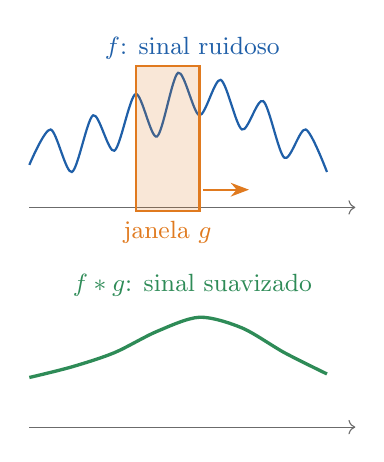
\begin{tikzpicture}[scale=0.9]
      % sinal ruidoso
      \draw[->,cinza] (0,0) -- (4.6,0);
      \draw[azul,thick] plot[smooth] coordinates
        {(0,0.6)(0.3,1.1)(0.6,0.5)(0.9,1.3)(1.2,0.8)(1.5,1.6)(1.8,1.0)(2.1,1.9)(2.4,1.3)(2.7,1.8)(3.0,1.1)(3.3,1.5)(3.6,0.7)(3.9,1.1)(4.2,0.5)};
      \node[azul,font=\small] at (2.3,2.25) {$f$: sinal ruidoso};
      % janela deslizante
      \fill[laranja,opacity=0.18] (1.5,-0.05) rectangle (2.4,2.0);
      \draw[laranja,thick] (1.5,-0.05) rectangle (2.4,2.0);
      \draw[-{Stealth},laranja,thick] (2.45,0.25) -- (3.1,0.25);
      \node[laranja,font=\small] at (1.95,-0.35) {janela $g$};
      % resultado
      \begin{scope}[yshift=-3.1cm]
        \draw[->,cinza] (0,0) -- (4.6,0);
        \draw[verde,very thick] plot[smooth] coordinates
          {(0,0.7)(0.6,0.85)(1.2,1.05)(1.8,1.35)(2.4,1.55)(3.0,1.4)(3.6,1.05)(4.2,0.75)};
        \node[verde,font=\small] at (2.3,2.0) {$f \conv g$: sinal suavizado};
      \end{scope}
    \end{tikzpicture}
  \end{columns}
  \intuicao{medições ruidosas são suavizadas por uma média ponderada, que pode pesar mais as recentes; no caso particular da média móvel de 7 dias da pandemia, os 7 pesos são iguais a $1/7$.}{Goodfellow et al., 2016, seç.~9.1}
\end{frame}

\begin{frame}{1.3\enspace Convolução como média ponderada}
  \begin{columns}[T]
    \column{0.5\textwidth}
    \small
    \begin{itemize}
      \item Um laser mede a posição de uma nave, com ruído: $x(t)$ é a posição medida no instante $t$.
      \item Para estimar a posição agora, faço uma \alert{média ponderada} das medições, pesando mais as recentes.
      \item Uma medição feita no instante $a$ tem idade $t-a$ e recebe peso $w(t-a)$.
      \item Fazendo isso em todo instante, saio com uma estimativa suavizada $s(t)$. \alert{Isso é uma convolução.}
    \end{itemize}
    \column{0.46\textwidth}
    \[ s(t)=\int x(a)\,w(t-a)\,da \qquad (9.1) \]
    \[ s(t)=(x\conv w)(t) \qquad (9.2) \]
    \begin{block}{Restrições do exemplo, não da definição}
      \footnotesize
      $w$ deve ser uma densidade (senão não é média) e $w(a)=0$ para $a<0$ (não olha o futuro).
      Em geral, a convolução vale para quaisquer funções em que a integral exista.
    \end{block}
  \end{columns}
  \vspace{0.3em}
  \centering\small
  Terminologia: $x$ = \textbf{entrada}, \ $w$ = \textbf{kernel}, \ $s$ = \textbf{mapa de características}.
  \intuicao{cada estimativa olha para trás e pondera as medições pela idade: o kernel diz quanto cada medição antiga ainda conta.}{Goodfellow et al., 2016, seç.~9.1, pp.~327--328}
\end{frame}

\begin{frame}{1.4\enspace A definição contínua}
  \[
    \boxed{\;(f \conv g)(t) \;=\; \int_{-\infty}^{\infty} f(\tau)\, g(t-\tau)\, d\tau\;}
  \]
  \begin{itemize}\small
    \item Esta é a definição geral.
    \item O $\tau$ (variável de integração) percorre o eixo; o $t$ é onde estou avaliando o resultado.
    \item O termo $g(t-\tau)$ é o $g$ \textbf{espelhado}, por causa do menos $\tau$, e \textbf{deslocado} até $t$.
    \item Multiplico pelo $f$ e integro: sai \alert{um número para cada $t$}. A integral existe (quase em toda parte), p.ex., se $f,g\in L^1(\mathbb{R})$.
  \end{itemize}
  \vspace{-0.2em}
  \centering
  \small Regra mnemônica: \textbf{espelhar $\to$ deslocar $\to$ multiplicar $\to$ integrar}\\
  \footnotesize\textcolor{cinza}{Oppenheim e Willsky (1997), seç.~2.2. Em Goodfellow et al.\ (2016, eq.~9.1): $s(t)=\int x(a)\,w(t-a)\,da$.}
  \intuicao{duas transparências: vire $g$ ao contrário, deslize-a sobre $f$ e, em cada posição $t$, a área sob o produto das curvas é o valor de $(f \conv g)(t)$.}{Oppenheim e Willsky, 1997, seç.~2.2}
\end{frame}

\begin{frame}{1.5\enspace Convolução em tempo contínuo: um exemplo}
  \small
  Exemplo: $f(\tau)=\text{pulso em }[0,1]$, \quad $g(\tau)=e^{-\tau}u(\tau)$, $u$ = degrau \quad(avaliando em $t=0{,}6$)
  \begin{columns}[T]
    \column{0.5\textwidth}
    \centering
    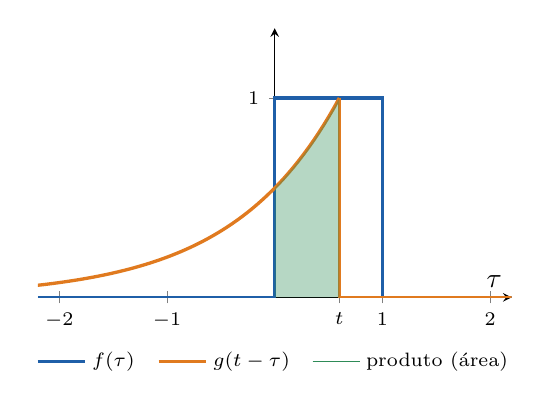
\begin{tikzpicture}
      \begin{axis}[width=7.6cm,height=5.0cm,
          axis lines=middle,xmin=-2.2,xmax=2.2,ymin=0,ymax=1.35,
          xlabel={$\tau$},xtick={-2,-1,0,0.6,1,2},
          xticklabels={$-2$,$-1$,$0$,$t$,$1$,$2$},ytick={1},
          tick label style={font=\scriptsize},legend columns=3,
          legend style={font=\scriptsize,at={(0.5,-0.16)},anchor=north,draw=none,fill=none,/tikz/every even column/.append style={column sep=6pt}}]
        \addplot[azul,very thick,const plot] coordinates {(-2.2,0)(0,1)(1,0)(2.2,0)};
        \addlegendentry{$f(\tau)$}
        \addplot[laranja,very thick,domain=-2.2:0.6,samples=60] {exp(-(0.6-x))};
        \addlegendentry{$g(t-\tau)$}
        \addplot[laranja,very thick,forget plot] coordinates {(0.6,1)(0.6,0)(2.2,0)};
        \addplot[verde,fill=verde,fill opacity=0.35,draw=none,domain=0:0.6,samples=40] {exp(-(0.6-x))} \closedcycle;
        \addlegendentry{produto (área)}
      \end{axis}
    \end{tikzpicture}
    \column{0.48\textwidth}
    \begin{enumerate}
      \item \textbf{Espelhar}: $g(\tau)\to g(-\tau)$.
      \item \textbf{Deslocar}: $g(-\tau)\to g(t-\tau)$.
      \item \textbf{Multiplicar}: $f(\tau)\,g(t-\tau)$.
      \item \textbf{Integrar}: a área verde é $(f\conv g)(t)$.
    \end{enumerate}
    \vspace{0.4em}
    Para $0\le t\le 1$:
    \[
      (f\conv g)(t)=\int_0^t e^{-(t-\tau)}d\tau = 1-e^{-t}
    \]
    Em $t=0{,}6$: $1-e^{-0{,}6}\approx 0{,}45$.
  \end{columns}
  \intuicao{$g(t-\tau)$ pondera o passado: o que entrou há $\Delta$ unidades de tempo pesa $e^{-\Delta}$. A área verde é a entrada acumulada até $t$, descontada por essa memória.}{Oppenheim e Willsky, 1997, seç.~2.2}
\end{frame}

\begin{frame}{1.6\enspace Exemplo clássico: pulso $\conv$ pulso $=$ triângulo}
  \begin{columns}[c]
    \column{0.55\textwidth}
    \centering
    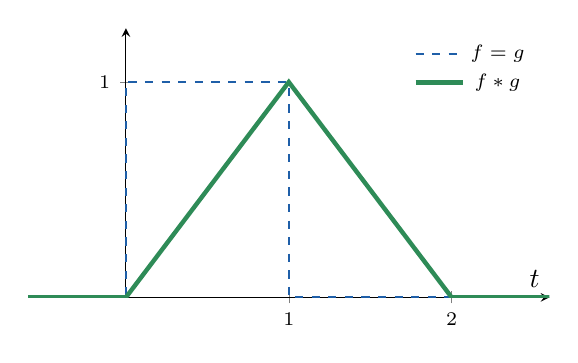
\begin{tikzpicture}
      \begin{axis}[width=8.2cm,height=5.0cm,
          axis lines=middle,xmin=-0.6,xmax=2.6,ymin=0,ymax=1.25,
          xlabel={$t$},xtick={0,1,2},ytick={1},tick label style={font=\scriptsize},
          legend style={font=\scriptsize,at={(0.98,0.98)},anchor=north east,draw=none,fill=none}]
        \addplot[azul,thick,dashed,const plot] coordinates {(-0.6,0)(0,1)(1,0)(2.6,0)};
        \addlegendentry{$f=g$}
        \addplot[verde,ultra thick] coordinates {(-0.6,0)(0,0)(1,1)(2,0)(2.6,0)};
        \addlegendentry{$f\conv g$}
      \end{axis}
    \end{tikzpicture}
    \column{0.42\textwidth}
    \[
      (f\conv f)(t)=
      \begin{cases}
        t, & 0\le t\le 1\\
        2-t, & 1\le t\le 2\\
        0, & \text{caso contrário}
      \end{cases}
    \]
    \begin{itemize}\small
      \item Deslizando um pulso sobre outro, a área de sobreposição cresce linearmente, chega ao máximo quando os dois coincidem, em $t=1$, e cai. Resultado: \alert{um triângulo de 0 a 2}.
      \item Suporte: $\operatorname{supp}(f\conv g)\subseteq\operatorname{supp}f+\operatorname{supp}g$; aqui, \alert{$[0,1]+[0,1]=[0,2]$}.
    \end{itemize}
  \end{columns}
\end{frame}

\begin{frame}{1.7\enspace Do contínuo ao discreto}
  \begin{itemize}
    \item Um sensor real mede em intervalos regulares (p.ex., 1 vez por segundo): $t$ passa a ser \alert{inteiro}.
      \[ s(t)=(x\conv w)(t)=\sum_{a=-\infty}^{\infty} x(a)\,w(t-a) \qquad (9.3) \]
    \item Em aprendizado de máquina, a entrada é um \alert{tensor} de dados e o kernel, um tensor de \alert{parâmetros aprendidos}.
    \item Só guardamos um número finito de valores; fora deles, entrada e kernel valem zero.
      Por isso, a soma infinita vira, na prática, uma \textbf{soma finita}.
  \end{itemize}
  \intuicao{a soma infinita é só notação: na prática, o kernel tem poucos pesos não nulos, e a conta percorre só eles.}{Goodfellow et al., 2016, seç.~9.1, p.~328}
\end{frame}

\begin{frame}{1.8\enspace De 1D para 2D: o kernel desliza sobre a imagem}
  \[
    (I \conv K)(i,j) \;=\; \sum_{m}\sum_{n} I(i-m,\,j-n)\;K(m,n)
  \]
  \centering
  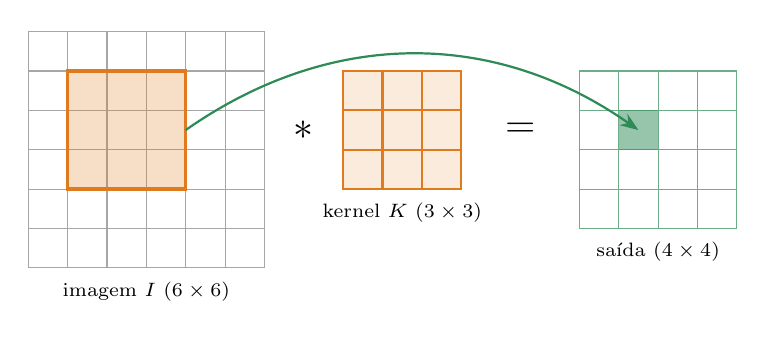
\begin{tikzpicture}[scale=0.5,every node/.style={font=\scriptsize}]
    % imagem 6x6
    \foreach \i in {0,...,5}
      \foreach \j in {0,...,5}
        \draw[cinza!60] (\i,\j) rectangle ++(1,1);
    \fill[laranja,opacity=0.25] (1,2) rectangle (4,5);
    \draw[laranja,very thick] (1,2) rectangle (4,5);
    \node[below] at (3,-0.1) {imagem $I$ ($6\times6$)};
    % kernel
    \begin{scope}[xshift=8cm,yshift=2cm]
      \foreach \i in {0,...,2}
        \foreach \j in {0,...,2}
          \draw[laranja,thick,fill=laranja!15] (\i,\j) rectangle ++(1,1);
      \node[below] at (1.5,-0.1) {kernel $K$ ($3\times3$)};
    \end{scope}
    \node at (7,3.5) {\Large $\conv$};
    % saída
    \begin{scope}[xshift=14cm,yshift=1cm]
      \foreach \i in {0,...,3}
        \foreach \j in {0,...,3}
          \draw[verde!70] (\i,\j) rectangle ++(1,1);
      \fill[verde,opacity=0.5] (1,2) rectangle (2,3);
      \node[below] at (2,-0.1) {saída ($4\times4$)};
    \end{scope}
    \node at (12.5,3.5) {\Large $=$};
    \draw[-{Stealth},verde,thick] (4,3.5) to[bend left=35] (15.5,3.5);
  \end{tikzpicture}

  \small Cada pixel de saída $=$ soma ponderada da vizinhança coberta pelo kernel; sem padding (\emph{valid}), a saída tem $(6-3+1)\times(6-3+1)=4\times4$ pixels.
  \textcolor{cinza}{(Goodfellow et al., 2016, eqs.~9.4--9.5)}
  \video{06_kernel_2d_curto}
  \intuicao{como passar uma lupa pela imagem: em cada posição, a janela $3\times3$ é resumida por um único número, a soma ponderada pelos pesos do kernel.}{Goodfellow et al., 2016, seç.~9.1}
\end{frame}

\begin{frame}{1.9\enspace Convolução em 2D: duas fórmulas equivalentes}
  \small
  Em imagens, a convolução corre em dois eixos. Por comutatividade, há duas formas:
  \[
    S(i,j)=\underbrace{\sum_m\sum_n I(m,n)\,K(i-m,\,j-n)}_{(9.4):\ m,n\ \text{indexam a imagem}}
    \;=\;\underbrace{\sum_m\sum_n I(i-m,\,j-n)\,K(m,n)}_{(9.5):\ m,n\ \text{indexam o kernel}}
  \]
  \vspace{-0.4em}
  \begin{columns}[T]
    \column{0.48\textwidth}
    \textbf{Na (9.4)}, com kernel $3\times3$ (índices $0,1,2$):\\
    só contribuem $m\in\{i-2,\,i-1,\,i\}$ e $n\in\{j-2,\,j-1,\,j\}$.
    \alert{O intervalo muda} a cada pixel de saída $(i,j)$, e ainda é cortado nas bordas da imagem.
    \column{0.48\textwidth}
    \textbf{Na (9.5)}, o intervalo é \alert{sempre o mesmo}: $m,n\in\{0,1,2\}$, os índices do kernel.
    O laço fica fixo, para qualquer $(i,j)$:\\[0.2em]
    \texttt{for m in 0..2: for n in 0..2:}\\
    \texttt{\ \ S[i,j] += I[i-m,j-n]*K[m,n]}
  \end{columns}
  \vspace{0.3em}
  \footnotesize A igualdade sai da troca de variável $m' = i-m$, $n' = j-n$.
  \intuicao{na (9.5), o laço percorre o kernel, que é pequeno e fixo; na (9.4), percorreria a parte da imagem sob o kernel, que muda a cada posição.}{Goodfellow et al., 2016, seç.~9.1, p.~328}
\end{frame}

\begin{frame}{1.10\enspace Espelhar ou não: a correlação cruzada}
  \begin{columns}[T]
    \column{0.52\textwidth}
    \footnotesize
    \begin{itemize}
      \item Na (9.5), quando $m$ \emph{cresce}, o índice da imagem $i-m$ \emph{decresce}: o kernel é percorrido \alert{espelhado}.
      \item O espelhamento dá à convolução propriedades algébricas, como a comutatividade (e a associatividade): úteis em provas, irrelevantes na implementação.
      \item Por isso, as bibliotecas calculam a \alert{correlação cruzada}, sem espelhar, e a chamam de ``convolução''.
    \end{itemize}
    \column{0.44\textwidth}
    \small
    Convolução:
    \[ S(i,j)=\sum_m\sum_n I(i-m,\,j-n)\,K(m,n) \]
    Correlação cruzada (9.6):
    \[ S(i,j)=\sum_m\sum_n I(i+m,\,j+n)\,K(m,n) \]
    \centering\footnotesize A única diferença: $-$ vira $+$.
  \end{columns}
  \begin{block}{E isso importa numa rede?}
    \small Não: com pesos aprendidos, a rede simplesmente aprende o kernel espelhado. E, com ReLU e pooling, ela já não comuta.
  \end{block}
  \intuicao{é a diferença entre ler o kernel da esquerda para a direita ou da direita para a esquerda; como a rede escolhe os pesos, ela se adapta a qualquer uma das leituras.}{Goodfellow et al., 2016, seç.~9.1, p.~329}
\end{frame}

\begin{frame}{1.11\enspace Um cálculo à mão --- e o detalhe do espelhamento}
  \small
  \begin{columns}[c]
    \column{0.3\textwidth}
    \centering
    Vizinhança $P$\\[0.3em]
    $\begin{bmatrix} 1&2&3\\4&5&6\\7&8&9 \end{bmatrix}$
    \column{0.3\textwidth}
    \centering
    Kernel Sobel $G_x$\\[0.3em]
    $\begin{bmatrix} -1&0&1\\-2&0&2\\-1&0&1 \end{bmatrix}$
    \column{0.36\textwidth}
    \textbf{Correlação} (sem espelhar):
    \[
      \textstyle\sum P\odot K = 2+4+2 = \textcolor{verde}{8}
    \]
    \textbf{Convolução} (kernel girado $180^\circ$):
    \[
      \textstyle\sum P\odot K^{\circlearrowleft} = \textcolor{laranja}{-8}
    \]
  \end{columns}
  \vspace{0.3em}
  \begin{alertblock}{Atenção}
    PyTorch \texttt{Conv2d} e TensorFlow calculam a \textbf{correlação cruzada}, $S(i,j)=\sum_{m,n} I(i+m,\,j+n)\,K(m,n)$.
    Como os pesos são aprendidos, a rede aprende o kernel já espelhado: os modelos são equivalentes.
    Para kernels fixos (Sobel), a distinção importa.
    \textcolor{cinza}{(Goodfellow et al., 2016, eq.~9.6; Zhang et al., 2023, seç.~7.2)}
  \end{alertblock}
  \video{07_espelhamento_2d}
  \intuicao{girar o kernel $180^\circ$ troca esquerda com direita e cima com baixo. Este Sobel é antissimétrico ($K^{\circlearrowleft}=-K$), por isso só o sinal muda; em geral, muda mais.}{Goodfellow et al., 2016, seç.~9.1}
\end{frame}

% =====================================================================
\section[2.\enspace Motivação (cap.~9.2)]{Motivação \textcolor{cinza}{(cap.~9.2)}}

\begin{frame}{2.1\enspace Três ideias: esparsidade, compartilhamento, equivariância}
  \begin{columns}[T]
    \column{0.52\textwidth}
    \begin{enumerate}
      \item \textbf{Interações esparsas}: cada saída depende só de uma vizinhança $K\times K$.
      \item \textbf{Compartilhamento de parâmetros}: o mesmo kernel é usado em todas as posições.
      \item \textbf{Equivariância à translação}: deslocar a entrada desloca a saída.
    \end{enumerate}
    \[
      \text{conv}\big(T(x)\big) = T\big(\text{conv}(x)\big),\quad T:\ \text{translação}
    \]
    \footnotesize\textcolor{cinza}{Não vale para rotação nem escala. Bordas e stride a tornam só aproximada (Azulay e Weiss, 2019).}
    \column{0.44\textwidth}
    \begin{block}{Quanto se economiza}
      Imagem $28\times 28$, saída do mesmo tamanho:\\[0.3em]
      camada densa: $\approx$ \textbf{615 mil pesos}\\
      convolução $3\times 3$: \alert{\textbf{9 pesos}}\\[0.3em]
      \textcolor{cinza}{Densa: $784\times784 = 614\,656$; convolução: os mesmos 9 pesos em todas as posições.}
    \end{block}
    \small Goodfellow et al.\ (2016), seç.~9.2; Zhang et al.\ (2023), seç.~7.1.
  \end{columns}
  \video{12_motivacao_curto}
  \intuicao{uma borda se decide pela vizinhança (esparsidade); um detector útil num lugar é útil em todos (compartilhamento); se o objeto se desloca, a resposta o acompanha.}{Goodfellow et al., 2016, seç.~9.2}
\end{frame}

\begin{frame}{2.2\enspace Interações esparsas: basta olhar a vizinhança}
  \centering
  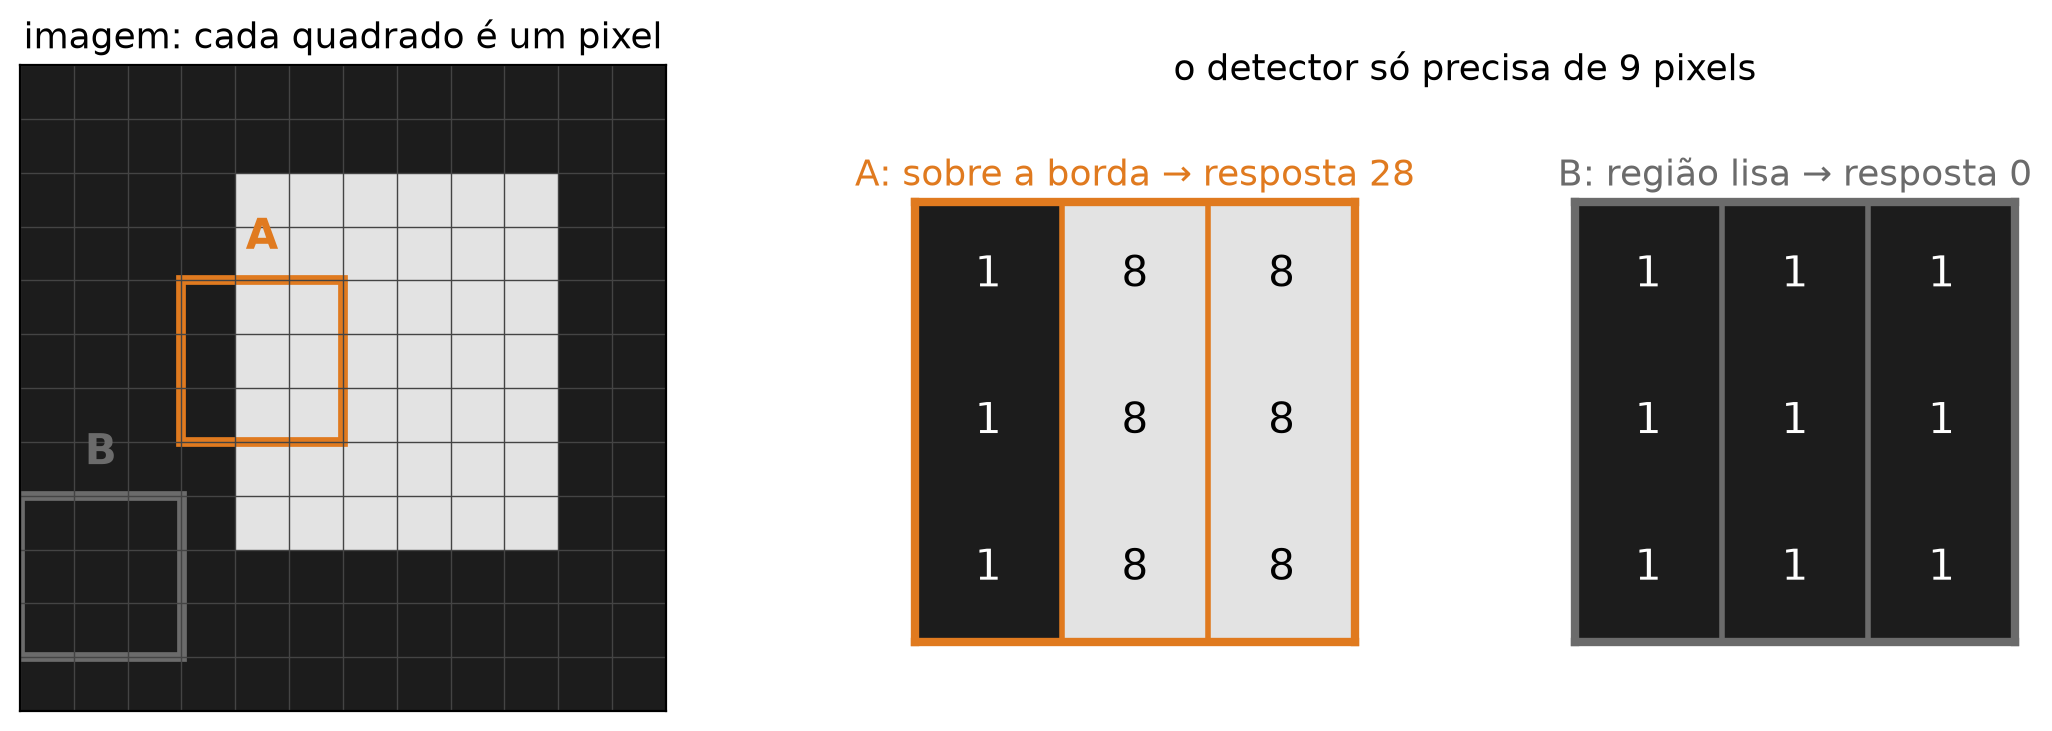
\includegraphics[width=0.82\linewidth]{figuras/esparsa.png}\\[0.4em]
  \begin{minipage}{0.92\linewidth}\small
    \begin{itemize}
      \item Cada saída depende só de uma \alert{vizinhança} da entrada: com o Sobel $G_x$, a janela $3\times3$ sobre a borda (A) dá 28; a da região lisa (B), 0.
      \item Com $m$ entradas e $n$ saídas, a camada densa usa $m\times n$ pesos e $O(m\times n)$ operações; com $k\ll m$ ligações por saída, \alert{$k\times n$} e $O(k\times n)$.
    \end{itemize}
  \end{minipage}
  \intuicao{para ver se há um degrau à frente, basta olhar o chão perto dos pés, não a sala inteira: a informação sobre uma borda está na vizinhança dela.}{Goodfellow et al., 2016, seç.~9.2, pp.~330--331}
\end{frame}

\begin{frame}{2.3\enspace Compartilhamento de parâmetros: um detector, todas as posições}
  \centering
  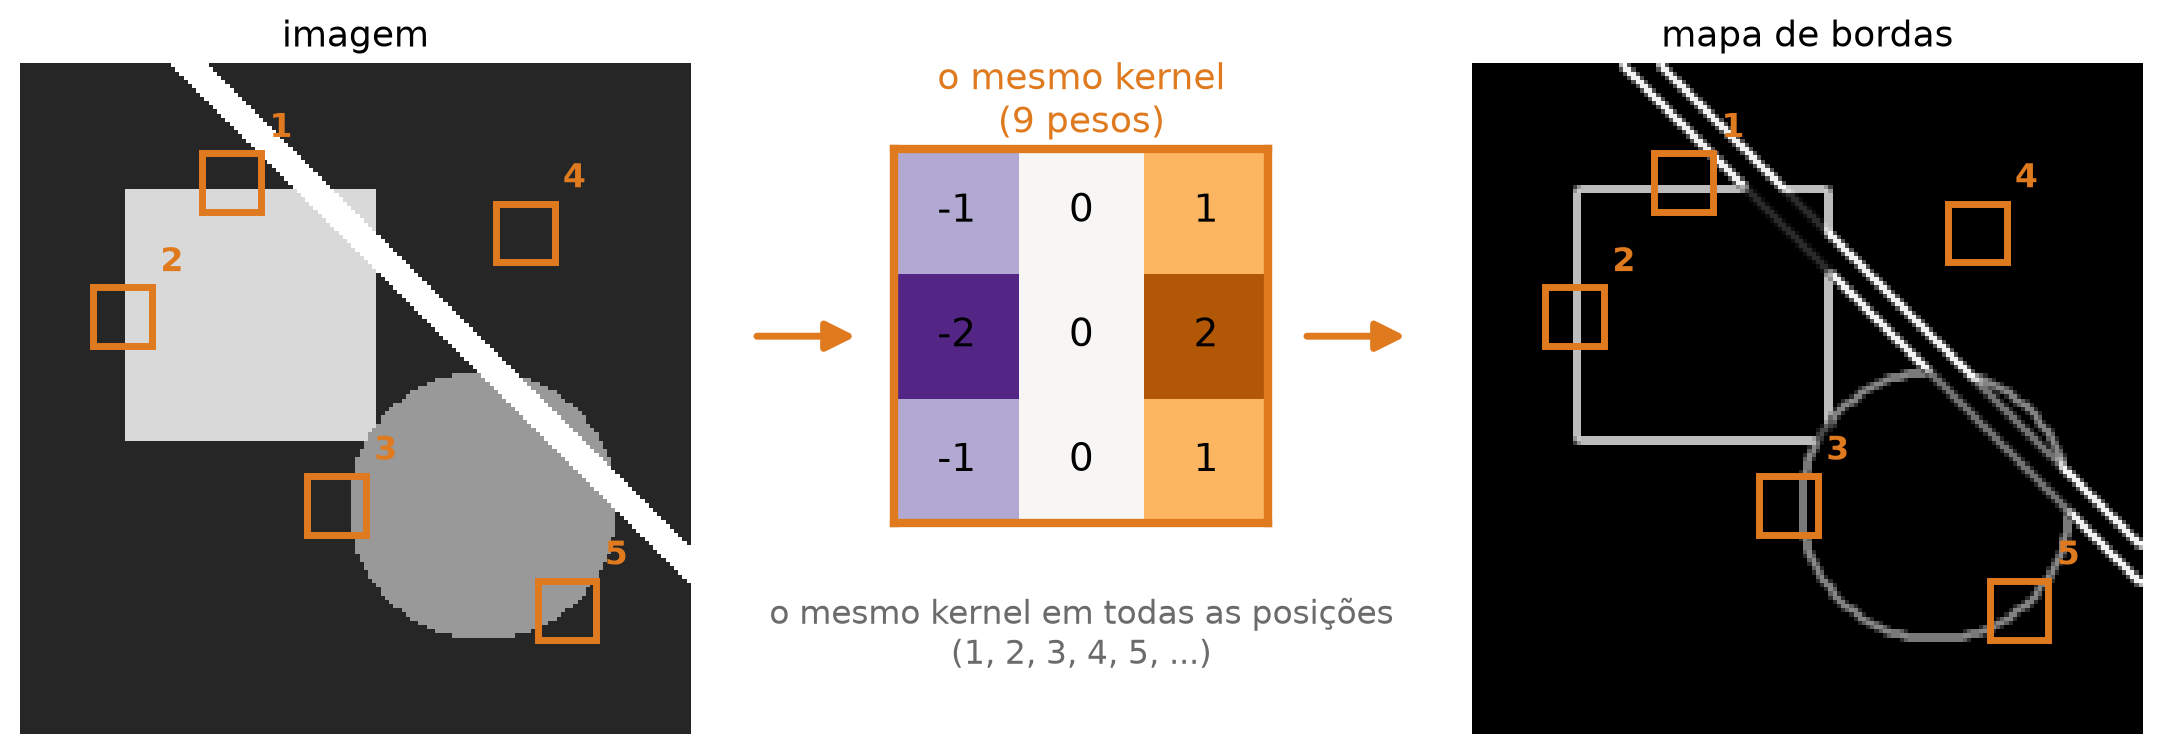
\includegraphics[width=0.9\linewidth]{figuras/compartilhamento.png}\\[0.8em]
  \begin{minipage}{0.88\linewidth}\centering
    Um detector de bordas útil num canto da imagem é útil em qualquer canto: basta aprendê-lo uma vez e
    reaproveitá-lo em todas as posições. São 9 pesos para a imagem inteira, de qualquer tamanho.
  \end{minipage}\\[0.4em]
  \footnotesize\textcolor{cinza}{Goodfellow et al.\ (2016), seç.~9.2.}
\end{frame}

\begin{frame}{2.4\enspace Equivariância à translação: o gato anda, a resposta anda junto}
  \centering
  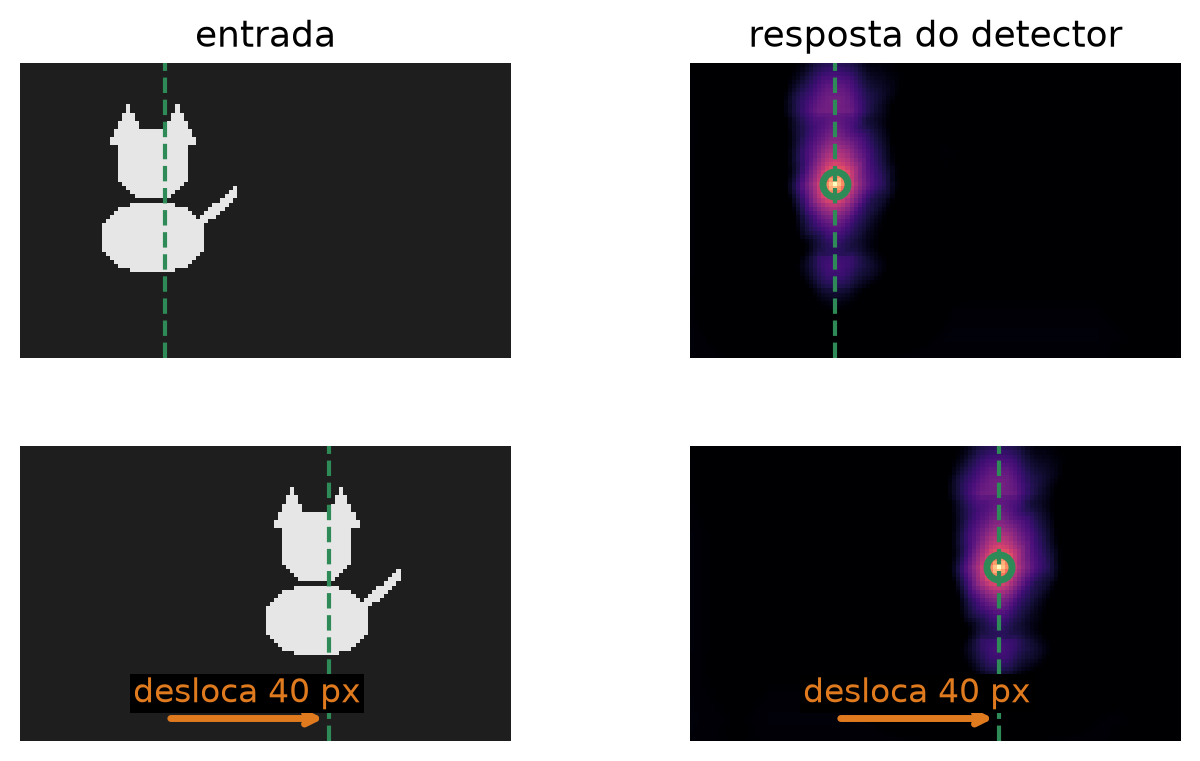
\includegraphics[width=0.56\linewidth]{figuras/gato.png}\\[0.4em]
  \begin{minipage}{0.88\linewidth}\centering
    Se o gato anda 40 pixels para a direita, o pico do detector anda os mesmos 40 pixels:
    deslocar e convoluir dá o mesmo que convoluir e deslocar. Não vale para rotação nem escala.
  \end{minipage}\\[0.4em]
  \footnotesize\textcolor{cinza}{Goodfellow et al.\ (2016), seç.~9.2. Detector: correlação com um modelo do gato.}
\end{frame}

\begin{frame}{2.5\enspace Campo receptivo}
  \begin{columns}[c]
    \column{0.5\textwidth}
    \centering
    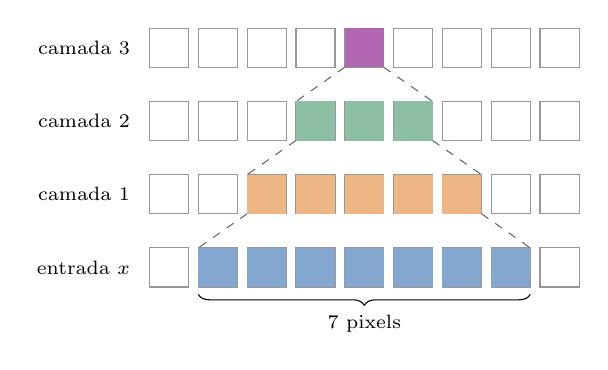
\begin{tikzpicture}[scale=0.62,every node/.style={font=\scriptsize}]
      \foreach \l/\cor/\nome in {0/azul/entrada $x$,1/laranja/camada 1,2/verde/camada 2,3/violet/camada 3} {
        \foreach \i in {0,...,8} \draw[cinza!70] (\i,1.5*\l) rectangle ++(0.8,0.8);
        \node[anchor=east] at (-0.2,1.5*\l+0.4) {\nome};
      }
      \fill[violet!60] (4,4.5) rectangle ++(0.8,0.8);
      \foreach \i in {3,4,5} \fill[verde!55] (\i,3) rectangle ++(0.8,0.8);
      \foreach \i in {2,...,6} \fill[laranja!55] (\i,1.5) rectangle ++(0.8,0.8);
      \foreach \i in {1,...,7} \fill[azul!55] (\i,0) rectangle ++(0.8,0.8);
      \draw[cinza,dashed] (4,4.5) -- (3,3.8); \draw[cinza,dashed] (4.8,4.5) -- (5.8,3.8);
      \draw[cinza,dashed] (3,3) -- (2,2.3); \draw[cinza,dashed] (5.8,3) -- (6.8,2.3);
      \draw[cinza,dashed] (2,1.5) -- (1,0.8); \draw[cinza,dashed] (6.8,1.5) -- (7.8,0.8);
      \draw[decorate,decoration={brace,mirror,amplitude=4pt}] (1,-0.15) -- (7.8,-0.15) node[midway,below=4pt] {7 pixels};
    \end{tikzpicture}
    \column{0.46\textwidth}
    \footnotesize
    \begin{itemize}
      \item \textbf{Campo receptivo}: a região da entrada que influencia um neurônio.
      \item Cada camada (kernel 3) olha 3 vizinhos, que já olhavam outros 3: a região cresce 2 pixels por camada.
        Após $L$ camadas: $R = 1 + L\,(K-1) = 1+3\cdot2=7$.
      \item Camadas profundas ``enxergam'' regiões grandes com kernels pequenos.
      \item Redes treinadas: bordas $\to$ texturas $\to$ partes $\to$ objetos (Zeiler e Fergus, 2014).
    \end{itemize}
  \end{columns}
  \intuicao{notícia passada de vizinho em vizinho: cada um só fala com quem está do lado, mas, após algumas rodadas, a informação já veio de longe.}{Goodfellow et al., 2016, seç.~9.2, fig.~9.4}
\end{frame}

\begin{frame}{2.6\enspace Aplicação: por que a VGG usa só kernels $3\times3$}
  \small
  \textbf{VGG} (Simonyan e Zisserman, 2015): CNN do \emph{Visual Geometry Group} de Oxford, entre as melhores do desafio ImageNet 2014.
  Sua ideia central: em vez de kernels grandes, \alert{empilhar várias convoluções $3\times3$}.\\[0.6em]
  \begin{columns}[T]
    \column{0.48\textwidth}
    \begin{block}{Mesmo campo receptivo: $7\times7$}
      \footnotesize Pelo slide 2.5, 3 camadas $3\times3$ enxergam $7\times7$ pixels, o mesmo que 1 camada $7\times7$.
    \end{block}
    \column{0.48\textwidth}
    \begin{block}{Quantos pesos? ($C$ canais de entrada e de saída)}
      \footnotesize
      1 camada $K\times K$ tem $K^2 C^2$ pesos.\\
      $3\times(3\times3)$: $3\cdot 9\,C^2 = \alert{27\,C^2}$\\
      $1\times(7\times7)$: $49\,C^2$
    \end{block}
  \end{columns}
  \vspace{0.5em}
  \centering
  Resultado: \textbf{45\% menos pesos} e \textbf{três não linearidades} (ReLU) em vez de uma, o que deixa a função mais expressiva.\\[0.3em]
  \footnotesize\textcolor{cinza}{Simonyan e Zisserman (2015), seç.~2.3; Zhang et al.\ (2023), seç.~8.2.}
  \intuicao{três degraus pequenos levam à mesma altura de um degrau grande, com menos material, e cada degrau é uma chance de mudar de direção.}{Simonyan e Zisserman, 2015}
\end{frame}

% =====================================================================
\section[3.\enspace Pooling (cap.~9.3)]{Pooling \textcolor{cinza}{(cap.~9.3)}}

\begin{frame}{3.1\enspace Uma camada convolucional: três estágios}
  \centering
  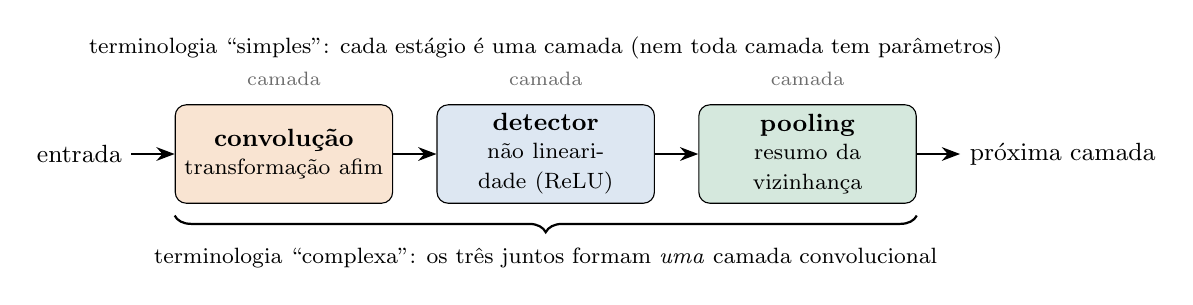
\begin{tikzpicture}[>={Stealth},font=\small,
      est/.style={draw,rounded corners,align=center,minimum height=1.25cm,text width=2.55cm,inner sep=3pt}]
    \node (e) {entrada};
    \node[est,fill=laranja!20,right=0.55cm of e] (c) {\textbf{convolução}\\[-1pt]\footnotesize transformação afim};
    \node[est,fill=azul!15,right=0.55cm of c] (d) {\textbf{detector}\\[-1pt]\footnotesize não linearidade (ReLU)};
    \node[est,fill=verde!20,right=0.55cm of d] (p) {\textbf{pooling}\\[-1pt]\footnotesize resumo da vizinhança};
    \node[right=0.55cm of p] (s) {próxima camada};
    \draw[->,thick] (e) -- (c); \draw[->,thick] (c) -- (d); \draw[->,thick] (d) -- (p); \draw[->,thick] (p) -- (s);
    \draw[decorate,decoration={brace,amplitude=6pt,mirror},thick] ([yshift=-0.15cm]c.south west) -- ([yshift=-0.15cm]p.south east)
      node[midway,below=8pt,font=\footnotesize,align=center] {terminologia ``complexa'': os três juntos formam \emph{uma} camada convolucional};
    \node[above=0.12cm of c,font=\scriptsize,cinza] {camada};
    \node[above=0.12cm of d,font=\scriptsize,cinza] {camada};
    \node[above=0.12cm of p,font=\scriptsize,cinza] {camada};
    \node[above=0.45cm of d,font=\footnotesize,align=center] {terminologia ``simples'': cada estágio é uma camada (nem toda camada tem parâmetros)};
  \end{tikzpicture}\\[1.0em]
  \small
  $\text{detector}_o(i,j) = \sigma\big( b_o + \textstyle\sum_{c}\sum_{m,n} X_c(i+m,\,j+n)\,K_{o,c}(m,n) \big)$\\[0.3em]
  Sem $\sigma$, empilhar convoluções equivaleria a uma única convolução (associatividade).
  \video{11_cnn_curto}
  \intuicao{uma linha de montagem com três postos: medir cada vizinhança com o kernel, deixar passar só as respostas positivas e, por fim, resumir cada região.}{Goodfellow et al., 2016, seç.~9.3, fig.~9.7}
\end{frame}

\begin{frame}{3.2\enspace Pooling: um resumo da vizinhança}
  \centering
  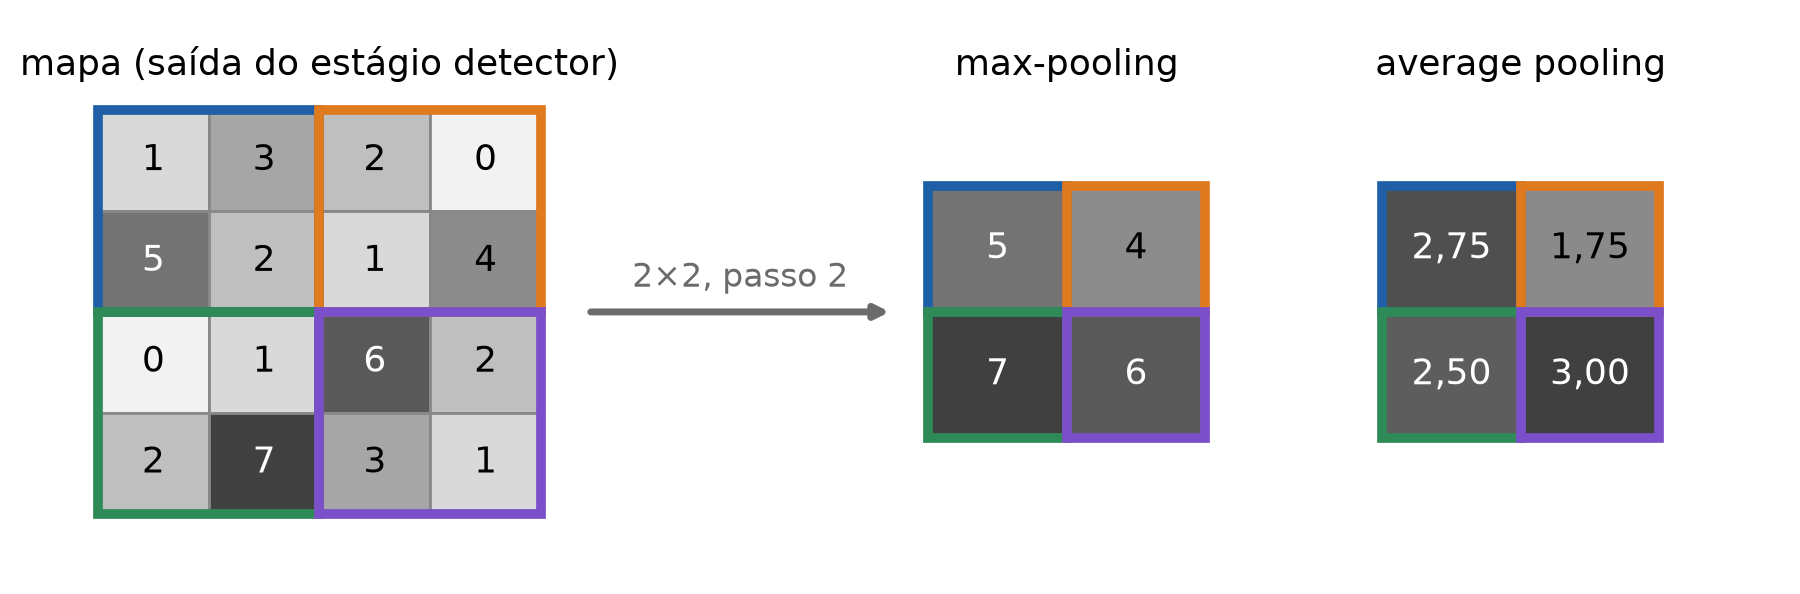
\includegraphics[width=0.84\linewidth]{figuras/pooling_def.png}\\[0.3em]
  \begin{minipage}{0.92\linewidth}\small
    A \alert{função de pooling} substitui a saída da rede numa posição por uma \textbf{estatística-resumo} das saídas vizinhas:
    o \textbf{máximo} (\emph{max pooling}), a \textbf{média} de uma vizinhança retangular, a \textbf{norma $L^2$} da vizinhança
    ou uma média ponderada pela distância ao pixel central. Não tem parâmetros a aprender.
  \end{minipage}
  \video{15_pooling_curto}
  \intuicao{a fase de grupos de um torneio: de cada grupo de 4, só o primeiro avança. Sabe-se quem foi forte em cada grupo, mas não em que posição jogou.}{Goodfellow et al., 2016, seç.~9.3}
\end{frame}

\begin{frame}{3.3\enspace Invariância a pequenas translações}
  \centering
  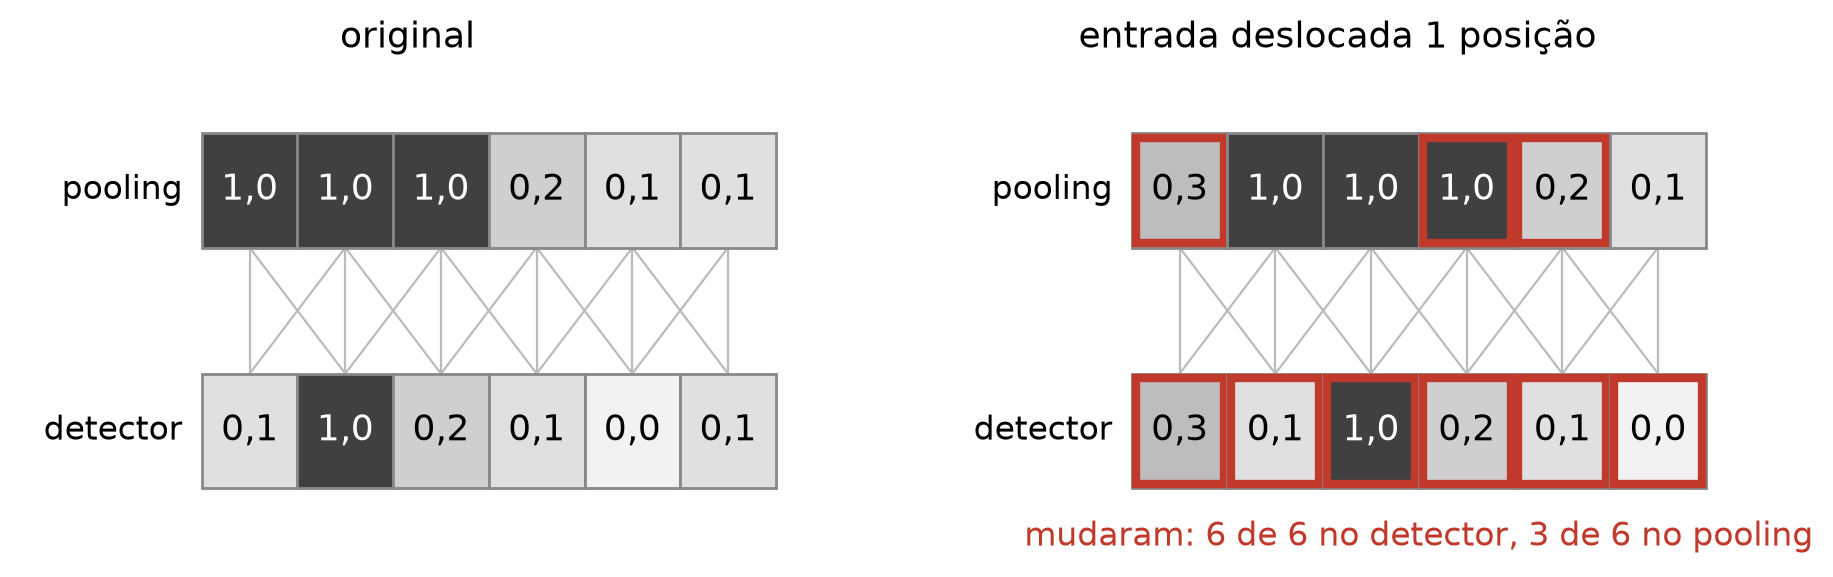
\includegraphics[width=0.62\linewidth]{figuras/pooling_invariancia.png}\\[0.1em]
  \begin{columns}[T]
    \column{0.5\textwidth}
    \footnotesize
    \begin{itemize}
      \item \textbf{Invariância}: com a entrada deslocada de uma posição, todas as saídas do detector mudam, mas só \emph{metade} das do pooling
        (a convolução é \emph{equivariante}: a saída se desloca junto).
      \item Útil quando importa mais \emph{se} a característica existe do que \emph{onde}: num rosto, basta um olho à esquerda e outro à direita.
    \end{itemize}
    \column{0.46\textwidth}
    \footnotesize
    \begin{itemize}
      \item Nem sempre: para achar um canto formado por duas bordas, a posição exata importa.
      \item O pooling impõe a invariância como certeza (um \emph{prior} infinitamente forte; ver 4.1): se a tarefa depende da posição exata, pode causar \emph{underfitting}.
    \end{itemize}
  \end{columns}
  \intuicao{um alarme de incêndio por cômodo: dispara com fumaça em qualquer canto, e mover a fumaça um pouco não muda nada; mas não diz em que canto ela está.}{Goodfellow et al., 2016, seç.~9.3--9.4}
\end{frame}

\begin{frame}{3.4\enspace Pooling entre canais: invariância aprendida à rotação}
  \begin{columns}[c]
    \column{0.46\textwidth}
    \centering
    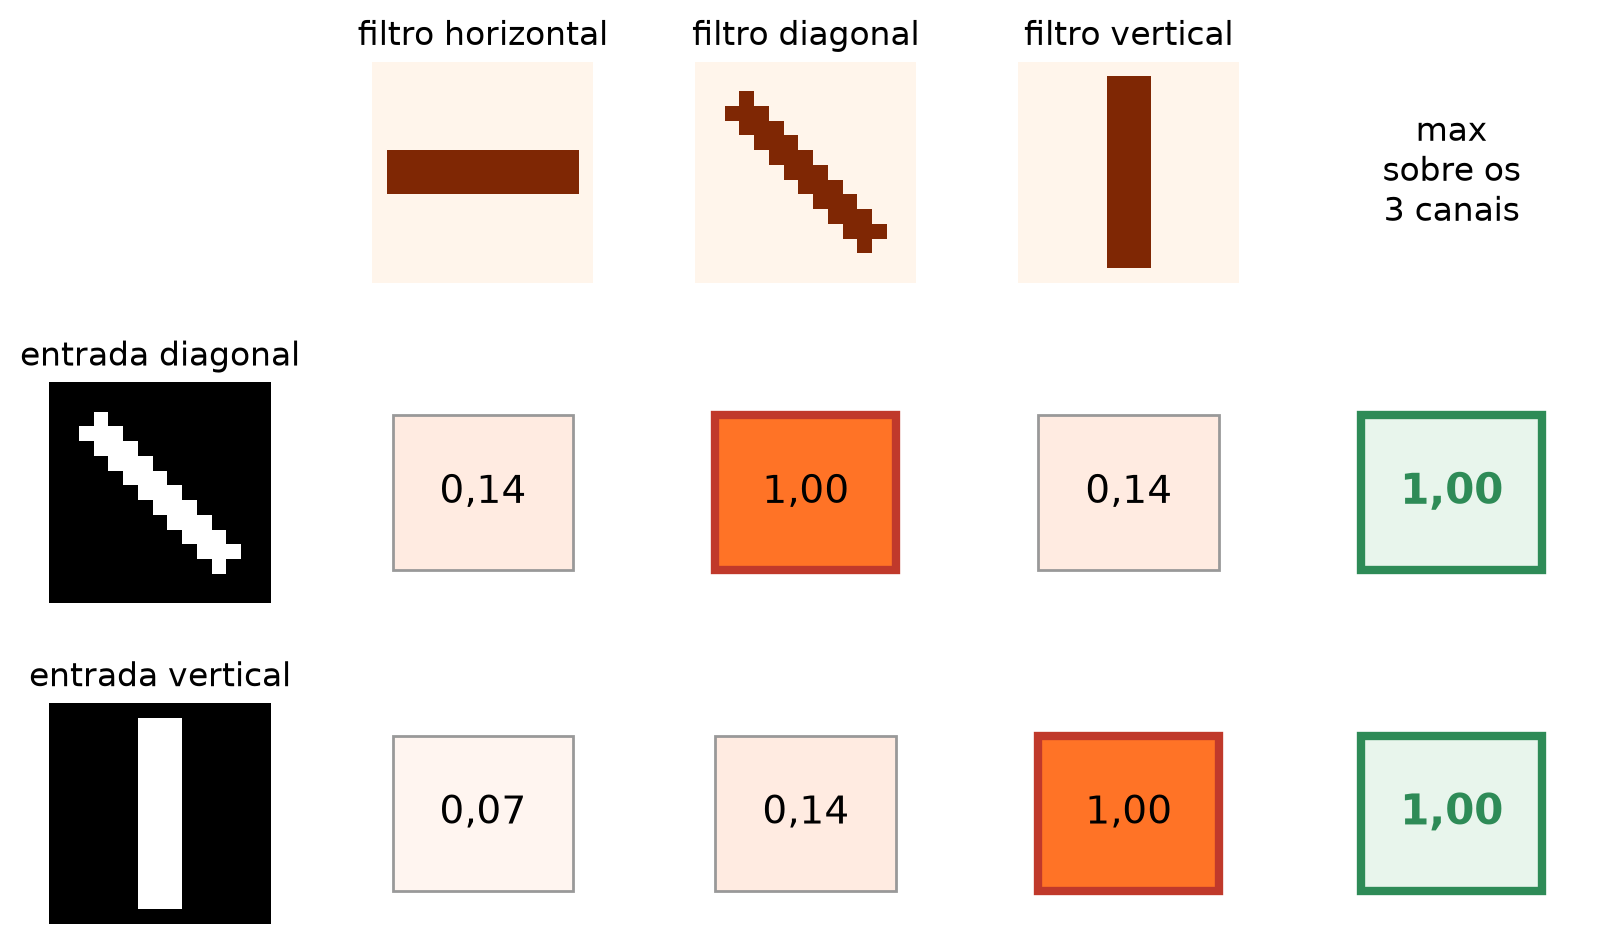
\includegraphics[width=\linewidth]{figuras/pooling_canais.png}
    \column{0.52\textwidth}
    \footnotesize
    \begin{itemize}
      \item Até aqui, o pooling resumia posições vizinhas de \emph{um} mapa. Ele também pode resumir \emph{vários mapas}, um por filtro.
      \item Três filtros procuram o mesmo traço em orientações diferentes. Cada número é o cosseno entre entrada e filtro: aqui, de 0 (nada) a 1 (idêntica), pois não há valores negativos.
      \item Cada entrada ativa um filtro diferente, mas o \alert{máximo} dos três é igual: a saída não muda quando o traço gira.
      \item Sozinha, a convolução não é invariante à rotação; com esse pooling, fica aproximadamente invariante às rotações cobertas pelos filtros (ideia das redes \emph{maxout}).
    \end{itemize}
  \end{columns}
  \intuicao{três vigias, cada um olhando numa direção: o alarme toca se qualquer um deles vir algo, não importa de que lado veio.}{Goodfellow et al., 2016, seç.~9.3, fig.~9.9; Goodfellow et al., 2013}
\end{frame}

\begin{frame}{3.5\enspace Pooling com passo e entradas de tamanho variável}
  \centering
  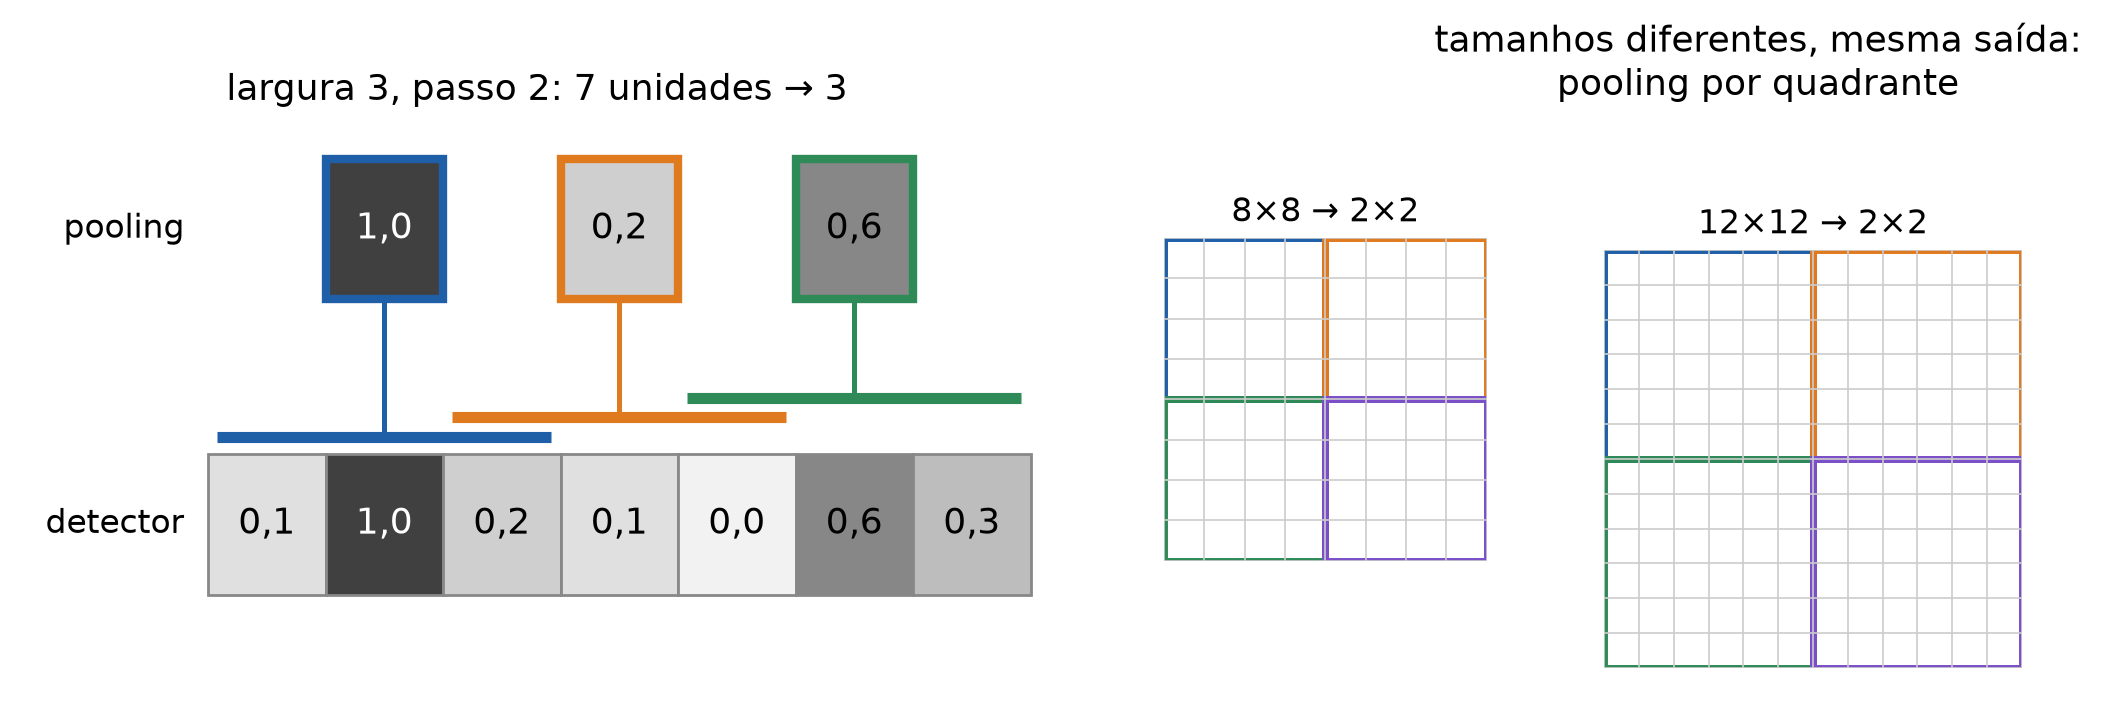
\includegraphics[width=0.86\linewidth]{figuras/pooling_stride.png}\\[0.3em]
  \begin{columns}[T]
    \column{0.48\textwidth}
    \footnotesize
    \textbf{Reduzir a resolução}: com regiões espaçadas de $k$ pixels, a camada seguinte recebe cerca de $k$ vezes menos entradas por dimensão ($k^2$ numa imagem):
    menos memória e menos computação.
    \column{0.48\textwidth}
    \footnotesize
    \textbf{Tamanho variável}: ajustando o espaçamento das regiões, o classificador recebe sempre o mesmo número de resumos;
    p.ex., um por quadrante, qualquer que seja o tamanho da imagem.
  \end{columns}
  \intuicao{resumir um livro em um parágrafo por capítulo: livros de tamanhos diferentes viram resumos do mesmo formato.}{Goodfellow et al., 2016, seç.~9.3, fig.~9.10}
\end{frame}

\begin{frame}{3.6\enspace Do pooling à arquitetura: três exemplos}
  \centering
  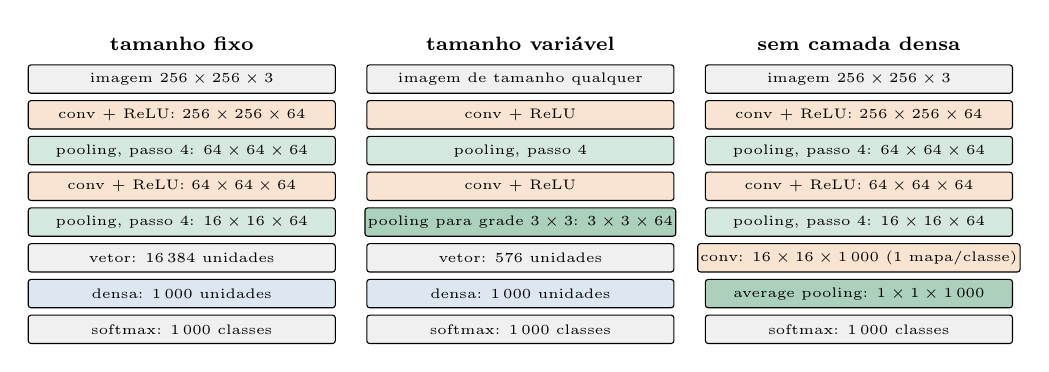
\begin{tikzpicture}[font=\tiny,>={Stealth},
      b/.style={draw,rounded corners=1pt,minimum width=3.9cm,minimum height=0.36cm,inner sep=1pt},
      cv/.style={b,fill=laranja!20}, pl/.style={b,fill=verde!20}, dn/.style={b,fill=azul!15}, io/.style={b,fill=cinza!10}]
    % (a) tamanho fixo
    \begin{scope}[xshift=0cm]
      \node[font=\scriptsize\bfseries] at (0,0.45) {tamanho fixo};
      \node[io] (a1) at (0,0) {imagem $256\times256\times3$};
      \node[cv,below=0.08cm of a1] (a2) {conv + ReLU: $256\times256\times64$};
      \node[pl,below=0.08cm of a2] (a3) {pooling, passo 4: $64\times64\times64$};
      \node[cv,below=0.08cm of a3] (a4) {conv + ReLU: $64\times64\times64$};
      \node[pl,below=0.08cm of a4] (a5) {pooling, passo 4: $16\times16\times64$};
      \node[io,below=0.08cm of a5] (a6) {vetor: 16\,384 unidades};
      \node[dn,below=0.08cm of a6] (a7) {densa: 1\,000 unidades};
      \node[io,below=0.08cm of a7] (a8) {softmax: 1\,000 classes};
    \end{scope}
    % (b) tamanho variável
    \begin{scope}[xshift=4.3cm]
      \node[font=\scriptsize\bfseries] at (0,0.45) {tamanho variável};
      \node[io] (b1) at (0,0) {imagem de tamanho qualquer};
      \node[cv,below=0.08cm of b1] (b2) {conv + ReLU};
      \node[pl,below=0.08cm of b2] (b3) {pooling, passo 4};
      \node[cv,below=0.08cm of b3] (b4) {conv + ReLU};
      \node[pl,below=0.08cm of b4,fill=verde!40] (b5) {pooling para grade $3\times3$: $3\times3\times64$};
      \node[io,below=0.08cm of b5] (b6) {vetor: 576 unidades};
      \node[dn,below=0.08cm of b6] (b7) {densa: 1\,000 unidades};
      \node[io,below=0.08cm of b7] (b8) {softmax: 1\,000 classes};
    \end{scope}
    % (c) sem camada densa
    \begin{scope}[xshift=8.6cm]
      \node[font=\scriptsize\bfseries] at (0,0.45) {sem camada densa};
      \node[io] (c1) at (0,0) {imagem $256\times256\times3$};
      \node[cv,below=0.08cm of c1] (c2) {conv + ReLU: $256\times256\times64$};
      \node[pl,below=0.08cm of c2] (c3) {pooling, passo 4: $64\times64\times64$};
      \node[cv,below=0.08cm of c3] (c4) {conv + ReLU: $64\times64\times64$};
      \node[pl,below=0.08cm of c4] (c5) {pooling, passo 4: $16\times16\times64$};
      \node[cv,below=0.08cm of c5] (c6) {conv: $16\times16\times1\,000$ (1 mapa/classe)};
      \node[pl,below=0.08cm of c6,fill=verde!40] (c7) {average pooling: $1\times1\times1\,000$};
      \node[io,below=0.08cm of c7] (c8) {softmax: 1\,000 classes};
    \end{scope}
  \end{tikzpicture}\\[0.5em]
  \footnotesize
  \textcolor{laranja!80!black}{$\blacksquare$} convolução \quad \textcolor{verde}{$\blacksquare$} pooling \quad \textcolor{azul}{$\blacksquare$} densa.
  No centro, o pooling garante o mesmo tamanho para qualquer entrada; à direita, o average pooling substitui a camada densa.
  \intuicao{convolução e pooling se alternam: cada par extrai padrões e encolhe a imagem; no fim, um classificador decide. Redes reais são maiores e mais ramificadas.}{Goodfellow et al., 2016, seç.~9.3, fig.~9.11}
\end{frame}

% =====================================================================
\section[4.\enspace Convolução e pooling como um prior infinitamente forte (cap.~9.4)]{Convolução e pooling como um prior infinitamente forte \textcolor{cinza}{(cap.~9.4)}}

\begin{frame}{4.1\enspace O que é um \emph{prior} infinitamente forte}
  \begin{columns}[T]
    \column{0.42\textwidth}
    \footnotesize
    \textbf{\emph{Prior}}: distribuição de probabilidade sobre os parâmetros que codifica o que achamos razoável \emph{antes} de ver os dados.\\[0.3em]
    \centering
    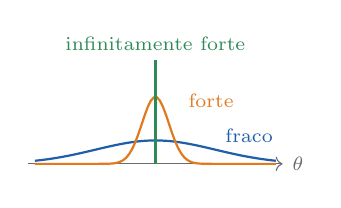
\begin{tikzpicture}[scale=0.85,every node/.style={font=\scriptsize}]
      \draw[->,cinza] (-1.9,0) -- (1.9,0) node[right] {$\theta$};
      \draw[azul,thick,domain=-1.8:1.8,samples=60] plot (\x,{0.35*exp(-\x*\x/1.6)});
      \draw[laranja,thick,domain=-1.8:1.8,samples=80] plot (\x,{1.0*exp(-\x*\x/0.08)});
      \draw[verde,very thick] (0,0) -- (0,1.55);
      \node[azul,anchor=west] at (0.9,0.42) {fraco};
      \node[laranja,anchor=west] at (0.35,0.95) {forte};
      \node[verde,anchor=south] at (0,1.55) {infinitamente forte};
    \end{tikzpicture}\\[0.2em]
    \raggedright
    Infinitamente forte: probabilidade \emph{zero} para alguns valores, que os dados não conseguem mudar.
    \column{0.54\textwidth}
    \footnotesize
    \begin{itemize}
      \item \textbf{Convolução} $=$ camada densa com um prior infinitamente forte: pesos \emph{zero} fora do campo receptivo e \emph{iguais} entre posições. A função só pode aprender interações locais e equivariantes à translação.
      \item \textbf{Pooling} $=$ prior infinitamente forte de \emph{invariância} a pequenas translações.
      \item Ou seja: essas propriedades não são aprendidas; são impostas pela arquitetura.
    \end{itemize}
  \end{columns}
  \intuicao{antes de ver qualquer foto, a CNN já ``acredita'' que o que importa é local e pode estar em qualquer lugar; nenhum dado consegue tirar essa crença dela.}{Goodfellow et al., 2016, seç.~9.4}
\end{frame}

\begin{frame}{4.2\enspace Consequências do \emph{prior} da convolução}
  \begin{columns}[T]
    \column{0.48\textwidth}
    \begin{block}{1. Pode causar \emph{underfitting}}
      \footnotesize
      Como todo prior, só ajuda se a suposição for razoável.
      \begin{itemize}
        \item Se a tarefa depende da \textbf{posição exata}, o pooling pode aumentar o erro de \emph{treino}. Algumas redes (Szegedy et al., 2014) aplicam pooling só em parte dos canais: umas características invariantes, outras precisas.
        \item Se a tarefa depende de \textbf{pontos muito distantes} da entrada, o prior local da convolução pode ser inadequado.
      \end{itemize}
    \end{block}
    \column{0.48\textwidth}
    \begin{block}{2. Só compare CNNs com CNNs}
      \footnotesize
      Um modelo sem convolução aprenderia igual se os pixels fossem embaralhados (sempre do mesmo jeito): ele é \emph{invariante a permutação} e precisa descobrir a topologia sozinho.
      A CNN já recebe pronta a noção de vizinhança. Por isso, há \emph{benchmarks} separados para os dois tipos.
    \end{block}
  \end{columns}
  \intuicao{um prior forte é um atalho: se a suposição vale, aprende-se com menos dados; se não vale, o atalho leva ao lugar errado.}{Goodfellow et al., 2016, seç.~9.4}
\end{frame}

% =====================================================================
\section[5.\enspace Variantes da função de convolução básica (cap.~9.5)]{Variantes da função de convolução básica \textcolor{cinza}{(cap.~9.5)}}

\begin{frame}{5.1\enspace Múltiplos canais de entrada e de saída}
  \begin{columns}[T]
    \column{0.52\textwidth}
    \begin{itemize}
      \item Entrada com $C_{\text{in}}$ canais $\Rightarrow$ cada filtro tem $C_{\text{in}}$ fatias $K\times K$.
      \item Convolui canal a canal e \alert{soma}, mais um viés:
    \end{itemize}
    \[ Y_o = \sum_{c=1}^{C_{\text{in}}} X_c \star K_{o,c} + b_o \]
    \vspace{-0.6em}\begin{center}\small $\star$: correlação cruzada, como nas bibliotecas.\end{center}
    \begin{itemize}
      \item $C_{\text{out}}$ filtros $\Rightarrow$ $C_{\text{out}}$ canais de saída.
    \end{itemize}
    \column{0.44\textwidth}
    \begin{block}{Número de parâmetros}
      \[ (K\cdot K\cdot C_{\text{in}} + 1)\cdot C_{\text{out}} \]
      \small RGB, $3\times 3$, 4 filtros: $(27+1)\cdot 4 = 112$.\\
      Não depende do tamanho da imagem.
    \end{block}
    \small Goodfellow et al.\ (2016), seç.~9.5; Zhang et al.\ (2023), seç.~7.4.
  \end{columns}
  \intuicao{cada filtro é uma pergunta feita a todos os canais da vizinhança de uma vez (``há aqui uma transição de vermelho para verde?''); cada filtro gera um mapa.}{Goodfellow et al., 2016, seç.~9.5}
\end{frame}

\begin{frame}{5.2\enspace Convolução $1\times 1$}
  \begin{columns}[c]
    \column{0.55\textwidth}
    \begin{itemize}
      \item Não olha vizinhos: em cada pixel, \alert{mistura os canais}.
      \item Equivale a uma camada densa aplicada pixel a pixel, com pesos compartilhados.
      \item Uso típico: reduzir ou aumentar o número de canais com pouco custo (NiN, GoogLeNet, ResNet).
    \end{itemize}
    \column{0.42\textwidth}
    \begin{block}{Parâmetros}
      \[ C_{\text{in}}\cdot C_{\text{out}} + C_{\text{out}} \]
      \small $256\to 64$: $256\cdot 64 + 64 = 16\,448$.
    \end{block}
    \small Lin et al.\ (2014); Zhang et al.\ (2023), seç.~7.4.
  \end{columns}
  \intuicao{como misturar tintas: em cada pixel, os $C_{\text{in}}$ valores são combinados linearmente, com proporções aprendidas e iguais em todos os pixels, sem olhar os vizinhos.}{Lin et al., 2014}
\end{frame}

\begin{frame}{5.3\enspace Padding e stride}
  \begin{columns}[T]
    \column{0.5\textwidth}
    \begin{itemize}
      \item \textbf{Padding} $P$: borda de zeros. Sem ela (\emph{valid}), cada camada perde $K-1$ pixels por dimensão.
      \item \textbf{Stride} $S$: o kernel pula $S$ posições; reduz a resolução.
    \end{itemize}
    \begin{block}{Tamanho da saída}
      \[ N_{\text{out}} = \left\lfloor \frac{N - K + 2P}{S} \right\rfloor + 1 \]
    \end{block}
    \column{0.46\textwidth}
    \small
    \begin{tabular}{cccc}
      \toprule
      $N$ & $K$ & $P,\,S$ & $N_{\text{out}}$ \\ \midrule
      5 & 3 & 0,\,1 & 3 \\
      5 & 3 & 1,\,1 & 5 \;(\emph{same}) \\
      5 & 3 & 1,\,2 & 3 \\
      224 & 7 & 3,\,2 & 112 \\
      \bottomrule
    \end{tabular}\\[0.4em]
    \textcolor{cinza}{Última linha: 1.\textsuperscript{a} camada da ResNet (He et al., 2016). Fórmula: Dumoulin e Visin (2016); Goodfellow et al.\ (2016), seç.~9.5; Zhang et al.\ (2023), seç.~7.3.}
  \end{columns}
  \intuicao{padding é uma moldura de zeros para que o kernel também se centre nos pixels da borda; stride $S$ avalia o kernel só a cada $S$ posições: menos avaliações, saída menor.}{Dumoulin e Visin, 2016}
\end{frame}

\begin{frame}{5.4\enspace Três tipos de \emph{zero padding}: \emph{valid}, \emph{same} e \emph{full}}
  \begin{columns}[c]
    \column{0.47\textwidth}
    \centering
    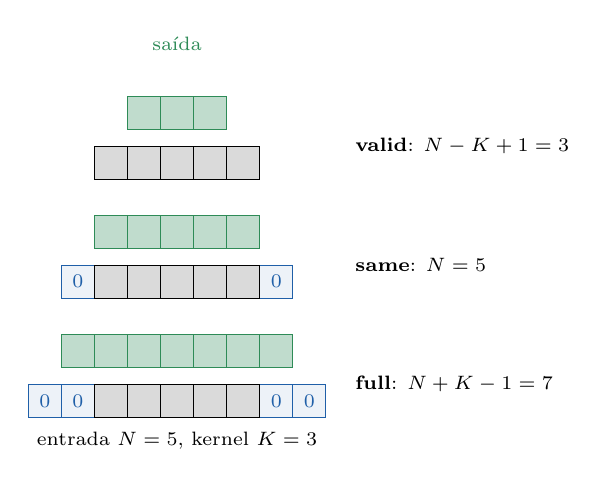
\begin{tikzpicture}[scale=0.42,every node/.style={font=\scriptsize}]
            \draw[fill=cinza!25] (0,7.2) rectangle ++(1,1);
      \draw[fill=cinza!25] (1,7.2) rectangle ++(1,1);
      \draw[fill=cinza!25] (2,7.2) rectangle ++(1,1);
      \draw[fill=cinza!25] (3,7.2) rectangle ++(1,1);
      \draw[fill=cinza!25] (4,7.2) rectangle ++(1,1);
      \draw[verde,fill=verde!30] (1,8.7) rectangle ++(1,1);
      \draw[verde,fill=verde!30] (2,8.7) rectangle ++(1,1);
      \draw[verde,fill=verde!30] (3,8.7) rectangle ++(1,1);
      \node[anchor=west] at (7.6,8.2) {\textbf{valid}: $N-K+1 = 3$};
      \draw[azul,fill=azul!8] (-1,3.6) rectangle ++(1,1); \node[azul] at (-0.5,4.1) {0};
      \draw[azul,fill=azul!8] (5,3.6) rectangle ++(1,1); \node[azul] at (5.5,4.1) {0};
      \draw[fill=cinza!25] (0,3.6) rectangle ++(1,1);
      \draw[fill=cinza!25] (1,3.6) rectangle ++(1,1);
      \draw[fill=cinza!25] (2,3.6) rectangle ++(1,1);
      \draw[fill=cinza!25] (3,3.6) rectangle ++(1,1);
      \draw[fill=cinza!25] (4,3.6) rectangle ++(1,1);
      \draw[verde,fill=verde!30] (0,5.1) rectangle ++(1,1);
      \draw[verde,fill=verde!30] (1,5.1) rectangle ++(1,1);
      \draw[verde,fill=verde!30] (2,5.1) rectangle ++(1,1);
      \draw[verde,fill=verde!30] (3,5.1) rectangle ++(1,1);
      \draw[verde,fill=verde!30] (4,5.1) rectangle ++(1,1);
      \node[anchor=west] at (7.6,4.6) {\textbf{same}: $N = 5$};
      \draw[azul,fill=azul!8] (-1,0) rectangle ++(1,1); \node[azul] at (-0.5,0.5) {0};
      \draw[azul,fill=azul!8] (5,0) rectangle ++(1,1); \node[azul] at (5.5,0.5) {0};
      \draw[azul,fill=azul!8] (-2,0) rectangle ++(1,1); \node[azul] at (-1.5,0.5) {0};
      \draw[azul,fill=azul!8] (6,0) rectangle ++(1,1); \node[azul] at (6.5,0.5) {0};
      \draw[fill=cinza!25] (0,0) rectangle ++(1,1);
      \draw[fill=cinza!25] (1,0) rectangle ++(1,1);
      \draw[fill=cinza!25] (2,0) rectangle ++(1,1);
      \draw[fill=cinza!25] (3,0) rectangle ++(1,1);
      \draw[fill=cinza!25] (4,0) rectangle ++(1,1);
      \draw[verde,fill=verde!30] (-1,1.5) rectangle ++(1,1);
      \draw[verde,fill=verde!30] (0,1.5) rectangle ++(1,1);
      \draw[verde,fill=verde!30] (1,1.5) rectangle ++(1,1);
      \draw[verde,fill=verde!30] (2,1.5) rectangle ++(1,1);
      \draw[verde,fill=verde!30] (3,1.5) rectangle ++(1,1);
      \draw[verde,fill=verde!30] (4,1.5) rectangle ++(1,1);
      \draw[verde,fill=verde!30] (5,1.5) rectangle ++(1,1);
      \node[anchor=west] at (7.6,1) {\textbf{full}: $N+K-1 = 7$};
      \node at (2.5,-0.7) {entrada $N=5$, kernel $K=3$};
      \node[verde] at (2.5,11.3) {saída};
    \end{tikzpicture}
    \column{0.5\textwidth}
    \footnotesize
    \begin{itemize}
      \item \textbf{\emph{Valid}} (sem zeros): o kernel só é aplicado onde cabe inteiro. A cada camada, a saída perde $K-1$ posições, o que limita a profundidade da rede.
      \item \textbf{\emph{Same}}: os zeros mantêm o tamanho, e a rede pode ter quantas camadas quiser. Porém, os pixels da borda influenciam menos saídas.
      \item \textbf{\emph{Full}}: cada pixel é visitado $K$ vezes. Porém, as saídas da borda dependem de poucos pixels, e é difícil um mesmo kernel funcionar bem em todas as posições.
      \item Em geral, a quantidade de zeros que dá a melhor acurácia de teste fica entre o \emph{valid} e o \emph{same}.
    \end{itemize}
  \end{columns}
  \intuicao{sem moldura, a foto encolhe a cada carimbo; com uma moldura de zeros, ela mantém o tamanho.}{Goodfellow et al., 2016, seç.~9.5, fig.~9.13}
\end{frame}

\begin{frame}{5.5\enspace Quanto compartilhar os pesos}
  \begin{columns}[c]
    \column{0.52\textwidth}
    \centering
    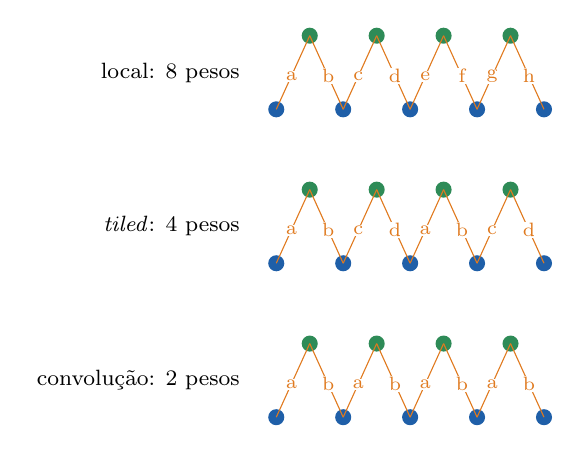
\begin{tikzpicture}[scale=0.85,every node/.style={font=\footnotesize}]
            \camada{4.6}{local: 8 pesos}{a,b,c,d,e,f,g,h}
      \camada{2.3}{\emph{tiled}: 4 pesos}{a,b,c,d,a,b,c,d}
      \camada{0}{convolução: 2 pesos}{a,b,a,b,a,b,a,b}
    \end{tikzpicture}\\[0.3em]
    \scriptsize 4 saídas, cada uma ligada a 2 entradas; letras iguais $=$ pesos iguais.
    \column{0.44\textwidth}
    \small
    Nas três, cada saída olha só a sua vizinhança. O que muda é \alert{quantas posições compartilham os mesmos pesos}:
    \begin{itemize}
      \item \textbf{localmente conectada}: nenhuma;
      \item \textbf{\emph{tiled}}: as posições se revezam entre $t$ kernels;
      \item \textbf{convolução}: todas.
    \end{itemize}
    Quanto mais compartilhamento, menos pesos para aprender, e mais forte a suposição de que um padrão vale em qualquer lugar.
  \end{columns}
  \intuicao{convolução: o mesmo carimbo em toda a imagem; localmente conectada: um carimbo por lugar; \emph{tiled}: um jogo de $t$ carimbos que se alternam.}{Goodfellow et al., 2016, seç.~9.5, fig.~9.16}
\end{frame}

\begin{frame}{5.6\enspace Convolução: um kernel para todas as posições}
  \centering
  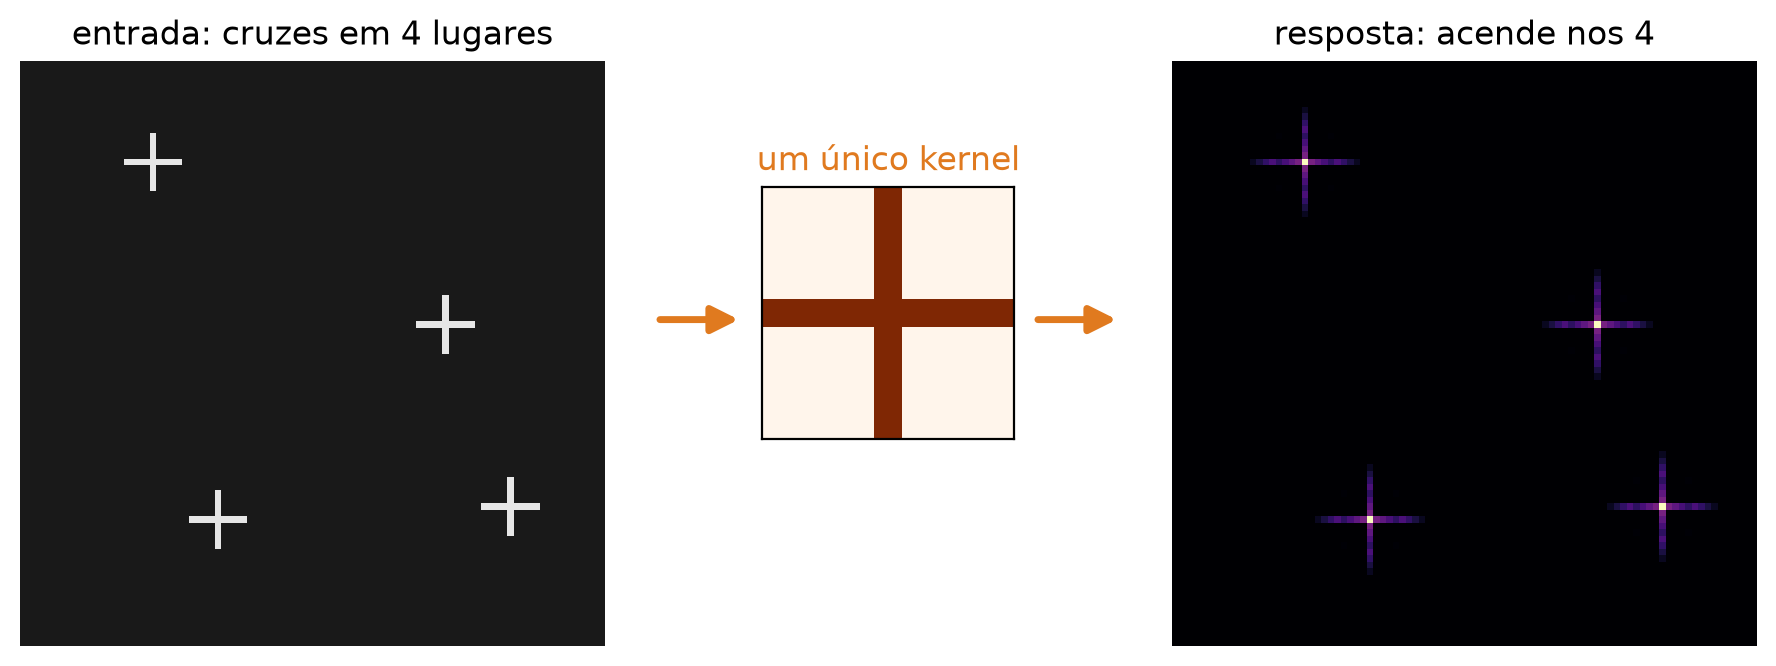
\includegraphics[width=0.8\linewidth]{figuras/var_conv.png}\\[0.6em]
  \begin{minipage}{0.88\linewidth}\centering\small
    O mesmo kernel percorre a imagem inteira. Por isso, ele encontra o padrão (aqui, uma cruz) em qualquer posição,
    e o número de pesos não depende do tamanho da imagem. É a escolha certa quando o padrão pode aparecer em qualquer lugar.
  \end{minipage}
  \intuicao{um único carimbo, procurado em toda a foto.}{Goodfellow et al., 2016, seç.~9.2 e 9.5}
\end{frame}

\begin{frame}{5.7\enspace Localmente conectada: pesos próprios para cada posição}
  \centering
  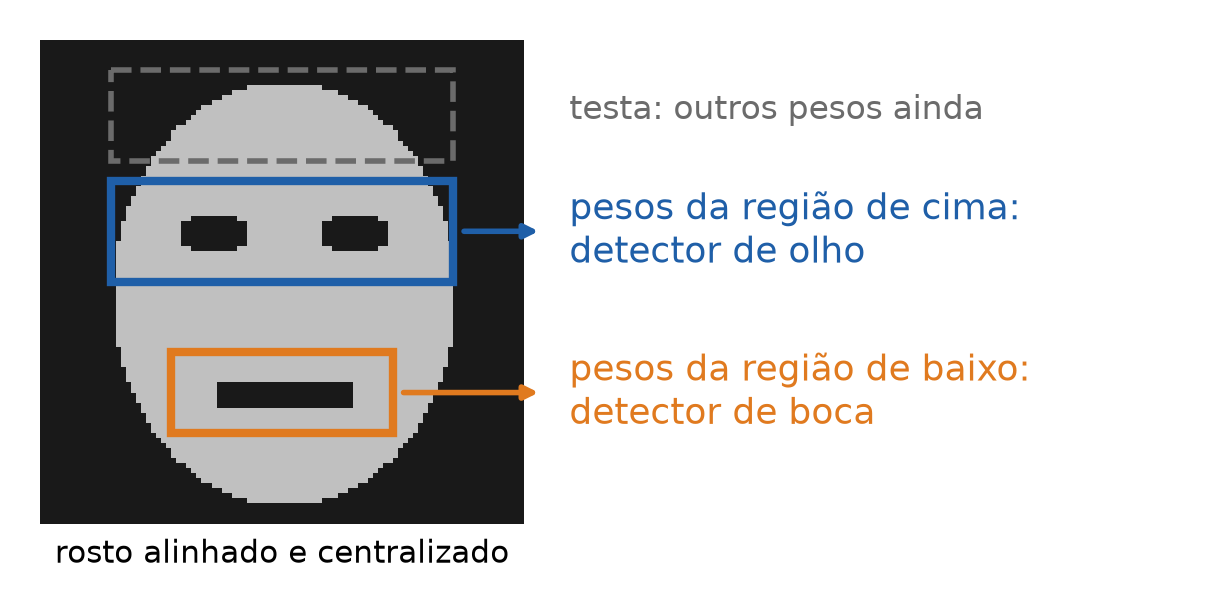
\includegraphics[width=0.66\linewidth]{figuras/var_local.png}\\[0.4em]
  \begin{minipage}{0.9\linewidth}\centering\small
    Também chamada de \emph{unshared convolution}: cada saída olha só a sua vizinhança, mas cada posição tem pesos próprios.
    Faz sentido quando a imagem está alinhada e cada característica só aparece numa região. Num rosto centralizado,
    os olhos ficam sempre em cima e a boca, embaixo; não há por que procurar a boca na testa.
  \end{minipage}
  \intuicao{um carimbo diferente para cada lugar da foto: cada região se especializa no que costuma aparecer nela.}{Goodfellow et al., 2016, seç.~9.5, fig.~9.14}
\end{frame}

\begin{frame}{5.8\enspace Convolução \emph{tiled}: um jogo de kernels em rodízio}
  \centering
  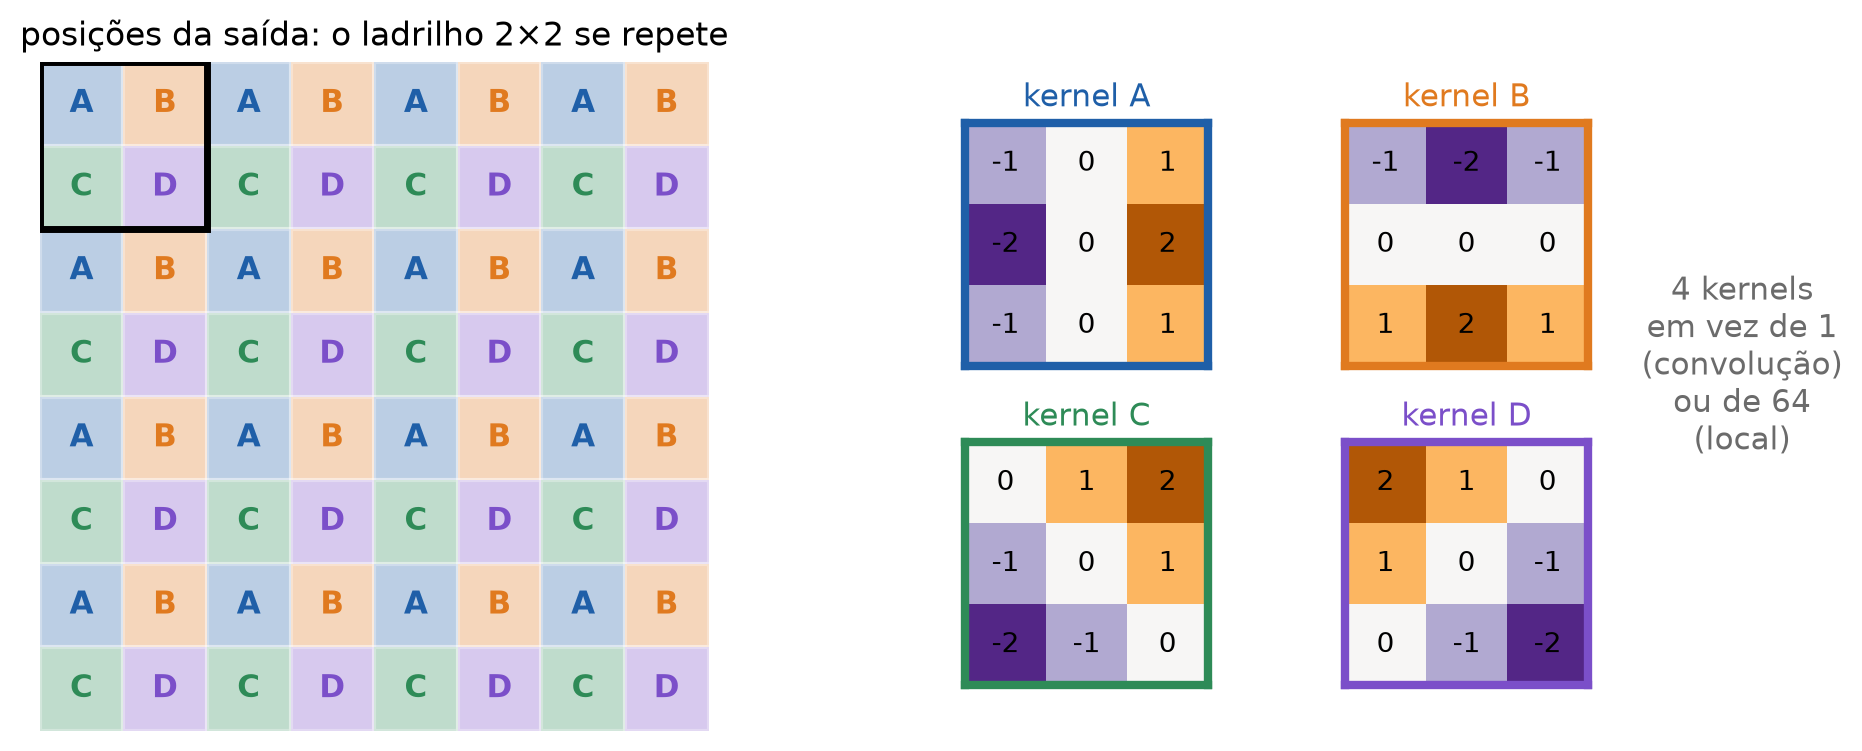
\includegraphics[width=0.74\linewidth]{figuras/var_tiled.png}\\[0.3em]
  \begin{minipage}{0.9\linewidth}\centering\small
    Aprende-se um conjunto de kernels, e cada posição usa um deles, seguindo um ladrilho que se repete.
    Com $t=2$ em cada direção, são 4 kernels: posições vizinhas usam kernels diferentes, mas o padrão se repete a cada 2 casas.
    É um meio-termo entre a convolução e a camada localmente conectada.
  \end{minipage}
  \intuicao{como o piso de ladrilhos: alguns desenhos diferentes, repetidos no mesmo padrão por todo o chão.}{Goodfellow et al., 2016, seç.~9.5, fig.~9.16}
\end{frame}

\begin{frame}{5.9\enspace Retropropagação numa camada convolucional}
  \centering
  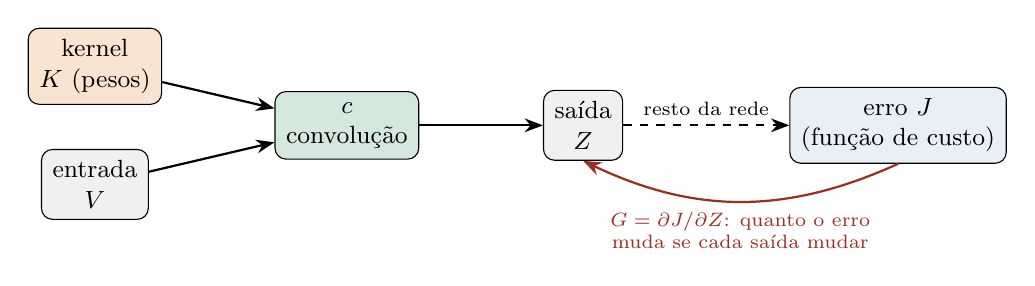
\begin{tikzpicture}[>={Stealth},font=\small,
      cx/.style={draw,rounded corners,minimum height=0.8cm,inner sep=4pt,align=center}]
    \node[cx,fill=cinza!10] (V) at (0,0) {entrada\\$V$};
    \node[cx,fill=laranja!20] (K) at (0,1.5) {kernel\\$K$ (pesos)};
    \node[cx,fill=verde!20] (c) at (3.2,0.75) {$c$\\convolução};
    \node[cx,fill=cinza!10] (Z) at (6.2,0.75) {saída\\$Z$};
    \node[cx,fill=azul!10] (J) at (10.2,0.75) {erro $J$\\(função de custo)};
    \draw[->,thick] (V) -- (c); \draw[->,thick] (K) -- (c); \draw[->,thick] (c) -- (Z);
    \draw[->,thick,dashed] (Z) -- node[above,font=\scriptsize] {resto da rede} (J);
    \draw[->,thick,vermelho!80!black] (J.south) to[bend left=25] node[below,font=\scriptsize,align=center]
      {$G = \partial J / \partial Z$: quanto o erro\\muda se cada saída mudar} (Z.south);
  \end{tikzpicture}\\[0.3em]
  \raggedright\footnotesize
  \textbf{Passagem direta}: $Z = c(K, V, s)$, em que $s$ é o passo (\emph{stride}).\\[0.3em]
  \textbf{Passagem de volta} (retropropagação): com $G$ em mãos, a camada calcula:
  \begin{itemize}
    \item $\partial J/\partial K = g(G, V, s)$ (eq.~9.12): quanto o erro muda com cada peso; serve para \alert{atualizar o kernel}.
    \item $\partial J/\partial V = h(K, G, s)$ (eq.~9.13): quanto o erro muda com cada entrada; é \alert{repassado} à camada anterior.
  \end{itemize}
  \intuicao{o erro chega de cima e se divide em duas partes: uma ajusta os pesos desta camada; a outra desce para a camada anterior, que faz o mesmo.}{Goodfellow et al., 2016, seç.~9.5, eqs.~9.11--9.13}
\end{frame}

\begin{frame}{5.10\enspace Convolução transposta e viés}
  \begin{columns}[c]
    \column{0.5\textwidth}
    \footnotesize
    Convolução (direta): $z = W\,v$
    \[
      \begin{bmatrix} z_1\\ z_2\\ z_3 \end{bmatrix} =
      \begin{bmatrix} w_1&w_2&w_3&0&0\\ 0&w_1&w_2&w_3&0\\ 0&0&w_1&w_2&w_3 \end{bmatrix}
      \begin{bmatrix} v_1\\ \vdots\\ v_5 \end{bmatrix}
    \]
    Volta (operação $h$): $\dfrac{\partial J}{\partial v} = W^{\top} G$, \ de 3 valores para 5.
    \column{0.46\textwidth}
    \footnotesize
    \begin{itemize}
      \item As três operações, $c$, $g$ e $h$, bastam para treinar qualquer rede convolucional \emph{feedforward}.
      \item Na matriz do slide B.8, a operação $h$ é a multiplicação pela \alert{transposta} $W^{\top}$. Por isso, ela é chamada de \emph{convolução transposta}.
      \item Como leva de menos para mais valores, ela também serve para \alert{aumentar a resolução}, como na reconstrução de autoencoders.
      \item \textbf{Viés}: em geral, há um por canal de saída, o mesmo em todas as posições.
    \end{itemize}
  \end{columns}
  \intuicao{a ida usa a matriz $W$; a volta, pelo mesmo caminho, usa a transposta $W^{\top}$.}{Goodfellow et al., 2016, seç.~9.5}
\end{frame}

\begin{frame}{5.11\enspace Exemplo: aprendendo um kernel por gradiente}
  \begin{columns}[T]
    \column{0.52\textwidth}
    \begin{itemize}\small
      \item Dados $X$ e o alvo $Y = X\star K_{\text{Sobel}}$, partimos de $K$ aleatório.
      \item Minimizamos $L(K) = \frac{1}{M}\lVert X\star K - Y\rVert^2$ por descida de gradiente.
      \item $L$ é quadrática e convexa em $K$; se a matriz das vizinhanças $3\times3$ de $X$ tem posto 9, o mínimo é único: o Sobel (300 passos aqui).
    \end{itemize}
    \column{0.44\textwidth}
    \begin{block}{O gradiente também é uma convolução}
      \[
        \nabla_K L = \tfrac{2}{M}\; X \star E,\qquad E = X\star K - Y
      \]
      \small Correlação da entrada com o erro, como na passagem direta (Goodfellow et al., 2016, seç.~9.5).
    \end{block}
    \footnotesize Adaptado de Zhang et al.\ (2023), seç.~7.2.4, que aprende o kernel $[1,\,-1]$.
  \end{columns}
  \video{17_aprendendo_kernel_curto}
  \intuicao{como afinar um violão: mede-se o erro (alto ou baixo?) e gira-se a tarraxa um pouco no sentido que o reduz; o gradiente dá esse sentido aos 9 pesos de uma vez.}{Goodfellow et al., 2016, seç.~4.3}
\end{frame}

% =====================================================================
\section[6.\enspace Saídas estruturadas (cap.~9.6)]{Saídas estruturadas \textcolor{cinza}{(cap.~9.6)}}

\begin{frame}{6.1\enspace Saídas estruturadas: um rótulo para cada pixel}
  \centering
  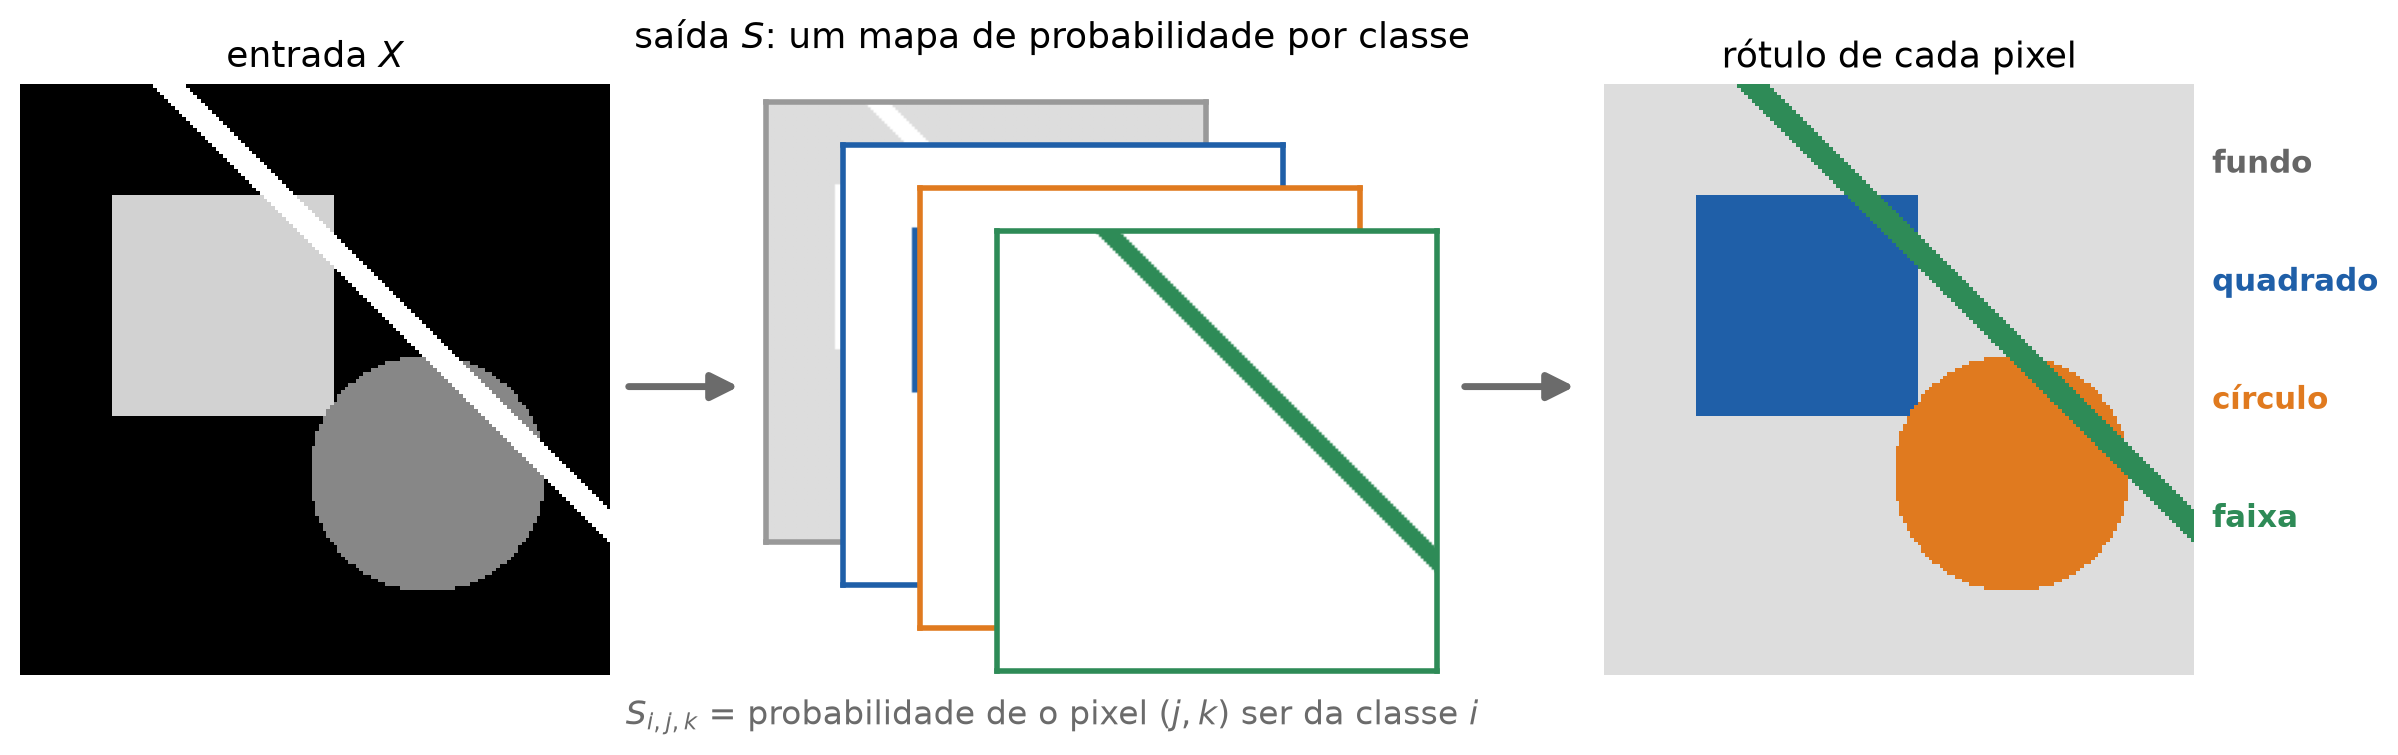
\includegraphics[width=0.86\linewidth]{figuras/segmentacao.png}\\[0.4em]
  \begin{minipage}{0.92\linewidth}\footnotesize
    Uma CNN não precisa devolver só um rótulo para a imagem inteira: ela pode devolver um \textbf{objeto estruturado}, como um tensor $S$,
    em que $S_{i,j,k}$ é a probabilidade de o pixel $(j,k)$ pertencer à classe $i$. Isso permite rotular cada pixel e desenhar o contorno de cada objeto
    (\emph{segmentação}).\\[0.3em]
    \textbf{Problema}: o pooling com passo grande deixa a saída menor que a entrada. \textbf{Soluções}: evitar o pooling, produzir uma grade de rótulos
    de resolução menor ou usar pooling com passo 1.
  \end{minipage}
  \intuicao{em vez de dizer ``nesta foto há um círculo'', a rede pinta cada pixel com a cor da sua classe, como num livro de colorir.}{Goodfellow et al., 2016, seç.~9.6}
\end{frame}

\begin{frame}{6.2\enspace Refinar o palpite: rede convolucional recorrente}
  \begin{columns}[c]
    \column{0.52\textwidth}
    \centering
    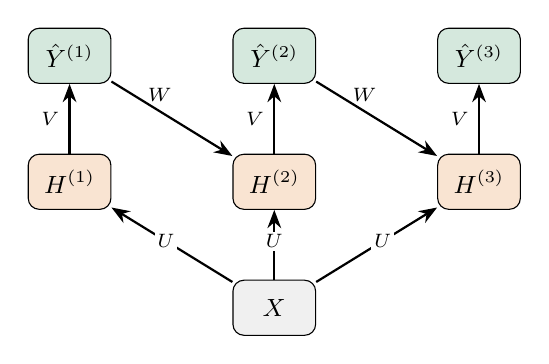
\begin{tikzpicture}[>={Stealth},font=\small,
        n/.style={draw,rounded corners,minimum width=1.05cm,minimum height=0.7cm,inner sep=2pt}]
      \node[n,fill=cinza!10] (X) at (2.6,0) {$X$};
      \foreach \t/\x in {1/0,2/2.6,3/5.2} {
        \node[n,fill=laranja!20] (H\t) at (\x,1.6) {$H^{(\t)}$};
        \node[n,fill=verde!20] (Y\t) at (\x,3.2) {$\hat Y^{(\t)}$};
        \draw[->,thick] (X) -- node[pos=0.55,font=\scriptsize,fill=white,inner sep=1pt] {$U$} (H\t);
        \draw[->,thick] (H\t) -- node[left,font=\scriptsize] {$V$} (Y\t);
      }
      \draw[->,thick] (Y1) -- node[above,font=\scriptsize,pos=0.4] {$W$} (H2);
      \draw[->,thick] (Y2) -- node[above,font=\scriptsize,pos=0.4] {$W$} (H3);
    \end{tikzpicture}\\[0.3em]
    \scriptsize os mesmos kernels $U$, $V$ e $W$ em todos os passos
    \column{0.44\textwidth}
    \footnotesize
    \begin{itemize}
      \item A rede faz um primeiro palpite $\hat Y^{(1)}$ para o rótulo de cada pixel.
      \item Depois, refina esse palpite várias vezes, olhando a entrada $X$ e o palpite anterior.
      \item Como os pesos são os mesmos em todos os passos, é uma \alert{rede recorrente} feita de convoluções (Pinheiro e Collobert, 2014).
      \item Em seguida, um pós-processamento agrupa pixels vizinhos com o mesmo rótulo em regiões contíguas, p.ex., com modelos gráficos.
    \end{itemize}
  \end{columns}
  \intuicao{como um esboço que se passa a limpo várias vezes: a cada passada, o desenho fica mais fiel à imagem.}{Goodfellow et al., 2016, seç.~9.6, fig.~9.17}
\end{frame}

% =====================================================================
\section[7.\enspace Tipos de dados (cap.~9.7)]{Tipos de dados \textcolor{cinza}{(cap.~9.7)}}

\begin{frame}{7.1\enspace Tipos de dados: dimensões e canais}
  \centering
  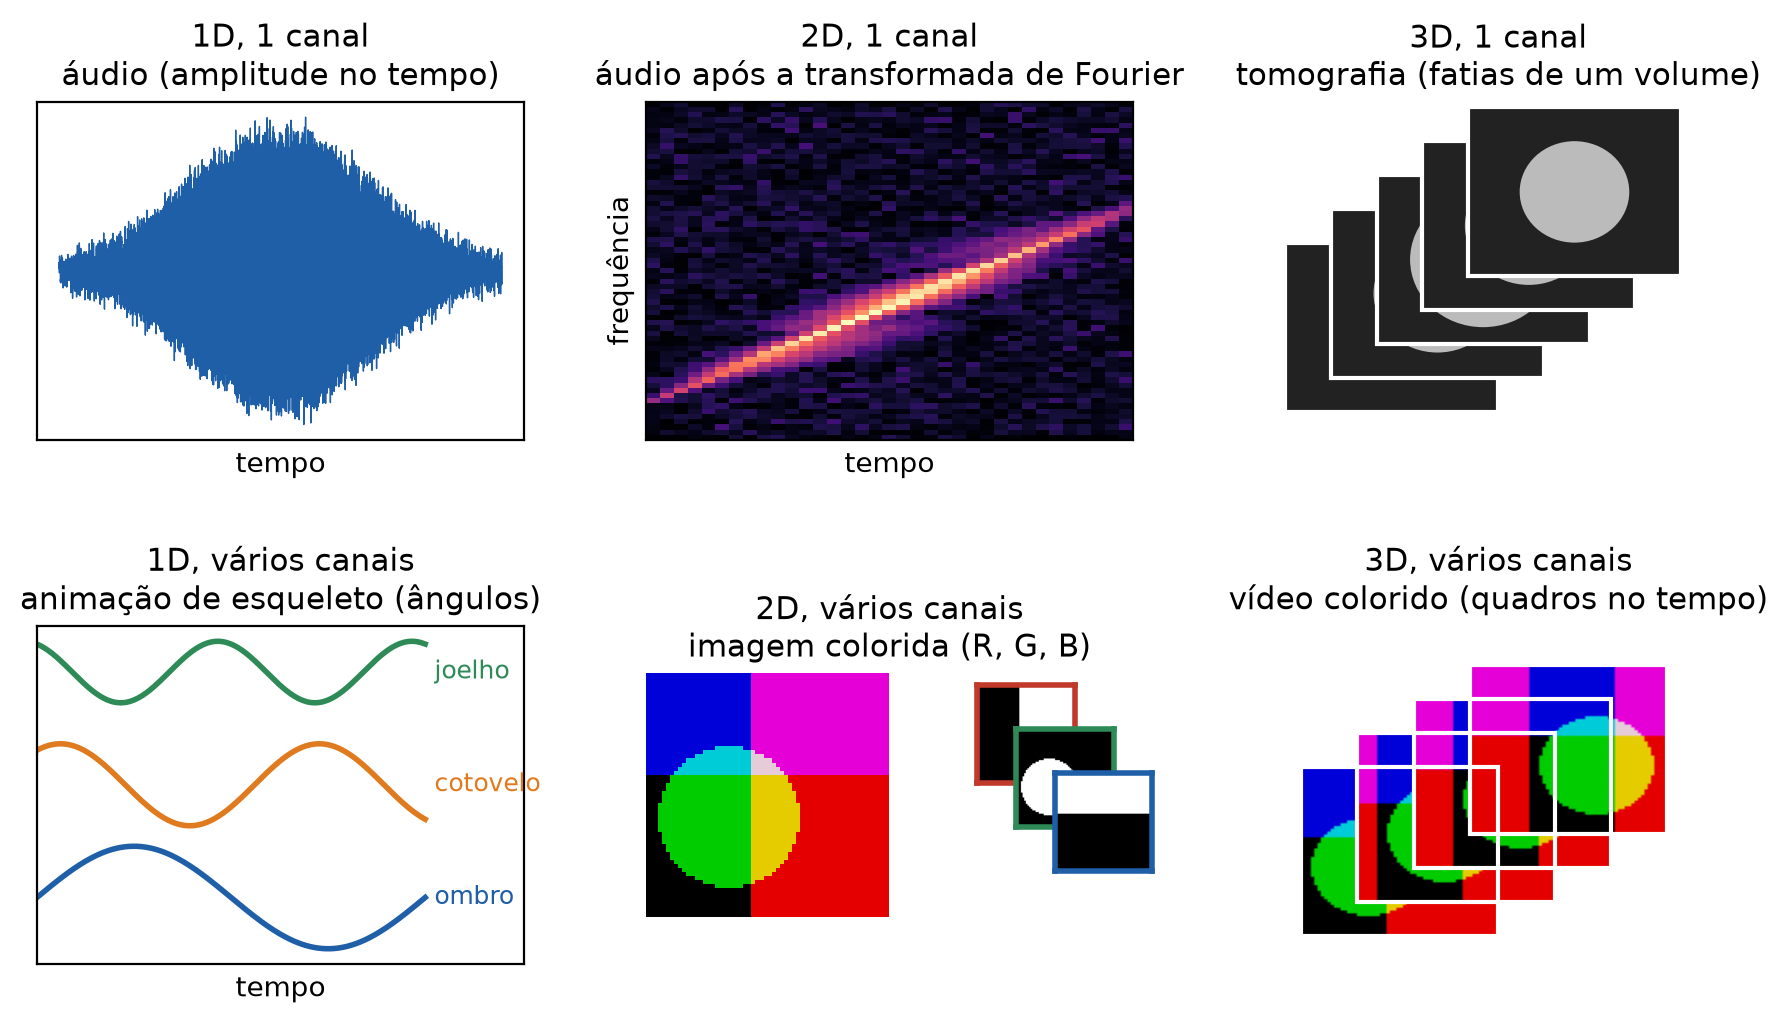
\includegraphics[width=0.6\linewidth]{figuras/tipos_dados.png}\\[0.3em]
  \begin{minipage}{0.94\linewidth}\footnotesize
    Os dados têm \textbf{dimensões} (tempo, espaço), ao longo das quais o kernel desliza, e \textbf{canais}: as grandezas medidas em cada ponto,
    que a convolução combina (seção 5.1). No espectrograma, convoluir também na frequência torna o modelo equivariante a deslocamentos de frequência.
  \end{minipage}
  \intuicao{dimensões são as ``direções'' em que o kernel desliza; canais são quantos números há em cada ponto.}{Goodfellow et al., 2016, seç.~9.7, tab.~9.1}
\end{frame}

\begin{frame}{7.2\enspace Entradas de tamanho variável}
  \centering
  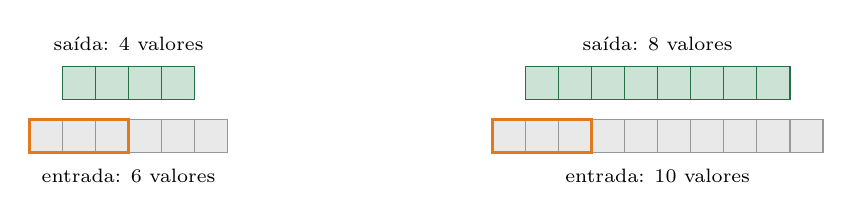
\begin{tikzpicture}[scale=0.42,every node/.style={font=\scriptsize}]
    \foreach \w/\x in {6/0, 10/14} {
      \foreach \i in {1,...,\w} \draw[cinza!70,fill=cinza!15] (\x+\i,0) rectangle ++(1,1);
      \pgfmathtruncatemacro{\n}{\w-2}
      \foreach \i in {1,...,\n} \draw[verde!80!black,fill=verde!25] (\x+\i+1,1.6) rectangle ++(1,1);
      \draw[laranja,very thick] (\x+1,0) rectangle ++(3,1);
      \node at (\x+\w/2+1,-0.7) {entrada: \w\ valores};
      \node at (\x+\w/2+1,3.3) {saída: \n\ valores};
    }
  \end{tikzpicture}\\[0.2em]
  \scriptsize o mesmo kernel de 3 pesos (laranja), aplicado em entradas de tamanhos diferentes\\[0.8em]
  \begin{columns}[T]
    \column{0.44\textwidth}
    \small
    \textbf{O problema}\\[0.2em]
    Uma camada densa tem um peso para cada valor da entrada. Por isso, ela só aceita entradas de um tamanho fixo.
    \column{0.44\textwidth}
    \small
    \textbf{A solução da convolução}\\[0.2em]
    O kernel é aplicado em cada posição. Numa entrada maior, ele é aplicado mais vezes, e a saída cresce; os pesos continuam os mesmos.
  \end{columns}
  \intuicao{o mesmo carimbo serve para folhas de qualquer largura: numa folha maior, basta carimbar mais vezes.}{Goodfellow et al., 2016, seç.~9.7}
\end{frame}

\begin{frame}{7.3\enspace Entradas de tamanho variável: quando a convolução se aplica}
  \begin{columns}[T]
    \column{0.47\textwidth}
    \centering
    \textcolor{verde}{\textbf{Aplica-se}}\\{\scriptsize\textcolor{verde}{observações do mesmo tipo}}\\[0.4em]
    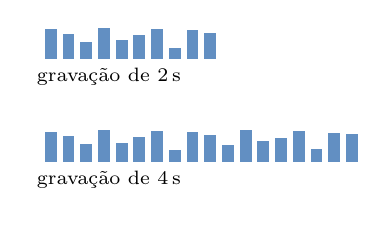
\begin{tikzpicture}[scale=0.5,every node/.style={font=\scriptsize}]
      \foreach \y/\n/\r in {2.6/10/gravação de 2\,s, 0/18/gravação de 4\,s} {
        \foreach \i in {1,...,\n} {
          \pgfmathsetmacro{\h}{0.25+0.55*abs(sin(\i*67))}
          \fill[azul!70] (\i*0.45,\y) rectangle ++(0.3,\h);
        }
        \node[anchor=west] at (0,\y-0.45) {\r};
      }
    \end{tikzpicture}\\[0.5em]
    \footnotesize
    A entrada varia em tamanho porque contém \emph{mais observações do mesmo tipo} ao longo de um eixo (tempo ou espaço).
    Toda posição tem a mesma semântica (amplitude num instante), o que justifica o \emph{compartilhamento de parâmetros}:
    o mesmo kernel é aplicado em todas as posições.
    \column{0.47\textwidth}
    \centering
    \textcolor{vermelho}{\textbf{Não se aplica}}\\{\scriptsize\textcolor{vermelho}{tipos distintos de observação}}\\[0.4em]
    \scriptsize
    \begin{tabular}{|l|l|}
      \hline
      \multicolumn{2}{|c|}{\textbf{candidato A}} \\ \hline
      média na graduação & 8,5 \\ \hline
    \end{tabular}\hspace{0.4em}%
    \begin{tabular}{|l|l|}
      \hline
      \multicolumn{2}{|c|}{\textbf{candidato B}} \\ \hline
      média na graduação & 7,9 \\ exame padronizado & 9,0 \\ \hline
    \end{tabular}\\[0.6em]
    \footnotesize
    A entrada de B é maior porque inclui uma observação \emph{opcional} de outro tipo (nem todo candidato fez o exame).
    Cada posição corresponde a um atributo distinto, logo não faz sentido convoluir os mesmos pesos sobre a média e sobre o exame.
  \end{columns}
  \intuicao{a convolução pressupõe que a mesma característica pode ocorrer em qualquer posição; numa ficha de inscrição, cada posição é uma pergunta diferente.}{Goodfellow et al., 2016, seç.~9.7}
\end{frame}

% =====================================================================
\section[8.\enspace Algoritmos eficientes de convolução (cap.~9.8)]{Algoritmos eficientes de convolução \textcolor{cinza}{(cap.~9.8)}}

\begin{frame}{8.1\enspace Por que buscar algoritmos eficientes}
  \small
  Aplicações modernas usam redes com \textbf{mais de um milhão de unidades} (valores dos mapas de características),
  e calcular cada unidade exige uma soma ponderada (uma aplicação do kernel): o custo cresce com o número de \emph{unidades}, e não só com o de parâmetros.\\[0.6em]
  \textbf{Ordem de grandeza.} Uma única camada $3\times3$ da VGG, com 64 canais de entrada e 64 de saída, sobre um mapa de $224\times224$:
  \[
    \underbrace{224\cdot 224}_{\text{posições}}\cdot\underbrace{64}_{\text{canais de saída}}\cdot
    \underbrace{3\cdot 3\cdot 64}_{\text{pesos por saída}}\;\approx\;1{,}85\times10^{9}\ \text{multiplicações por imagem.}
  \]
  \vspace{-0.3em}
  {\footnotesize Essa camada tem $224\cdot224\cdot64\approx3{,}2$ milhões de unidades, mas só $3\cdot3\cdot64\cdot64+64=36\,928$ parâmetros,
  graças ao compartilhamento de parâmetros (2.3).}
  \vspace{-0.4em}
  \begin{columns}[T]
    \column{0.48\textwidth}
    \begin{block}{Caminho 1: hardware}
      \footnotesize Implementações que exploram computação paralela (GPUs). É essencial, mas não muda o número de operações.
    \end{block}
    \column{0.48\textwidth}
    \begin{block}{Caminho 2: algoritmo}
      \footnotesize Reduzir o número de operações. Comparação em 8.2--8.3; cada método é detalhado nos slides de backup (B.1--B.5).
    \end{block}
  \end{columns}
  {\footnotesize\textcolor{cinza}{Goodfellow et al.\ (2016), seç.~9.8 e 12.1.2; Simonyan e Zisserman (2015).}}
\end{frame}

\begin{frame}{8.2\enspace Comparação de custo entre algoritmos}
  \small
  \textbf{O exemplo} é a camada do slide 8.1 (kernel $3\times3$, 64 canais), com $\approx3{,}2$ milhões de valores de saída.
  No cálculo direto, cada valor é uma soma de $3\cdot3\cdot64=576$ produtos. {\scriptsize\textcolor{cinza}{(Contagens calculadas; Lavin e Gray, 2016; Howard et al., 2017.)}}\\[0.5em]
  \centering
  \scriptsize
  \renewcommand{\arraystretch}{1.0}
  \begin{tabular}{@{}llrrl@{}}
    \toprule
    \textbf{método} & \textbf{como economiza} & \textbf{mult./saída} & \textbf{ganho} & \textbf{resultado} \\ \midrule
    direto & não economiza (referência) & 576 & $1\times$ & exato \\
    FFT (B.1--B.2) & convolução vira produto na frequência & $\approx210$ & $\approx2{,}7\times$ & exato \\
    kernel separável (B.3) & $3\times3$ vira $3\times1$ seguido de $1\times3$ & 384 & $1{,}5\times$ & exato$^{*}$ \\
    Winograd $F(2{\times}2,3{\times}3)$ (B.4) & troca produtos por somas & 256 & $2{,}25\times$ & exato \\
    Winograd $F(4{\times}4,3{\times}3)$ (B.4) & idem, com blocos maiores & 144 & $4\times$ & exato \\
    separável em profundidade (B.5) & cada canal sozinho, depois $1\times1$ & 73 & $7{,}9\times$ & \alert{outra camada} \\ \bottomrule
  \end{tabular}\\[0.2em]
  \raggedright
  \begin{itemize}
    \scriptsize
    \item \textbf{ganho} $=$ 576 $\div$ mult./saída. Na camada inteira ($\times$ 3,2 milhões): de $1{,}85\times10^{9}$ (direto) a $0{,}23\times10^{9}$ (em profundidade).
    \item $^{*}$Se o kernel for separável (posto 1), como o Sobel. FFT e Winograd: exatos a menos de arredondamento; Winograd sem as transformadas.
    \item FFT: estimativa com preenchimento até $256\times256$. Com 64 canais, cada FFT de entrada serve a 64 saídas: o custo das transformadas se dilui (num só sinal 1D, B.2, a FFT perde).
  \end{itemize}
\end{frame}

\begin{frame}{8.3\enspace Como ler a tabela: o que cada número esconde}
  \begin{columns}[T]
    \column{0.32\textwidth}
    \begin{block}{Exatos}
      \footnotesize
      \textbf{Direto, FFT, Winograd.} Calculam \emph{a mesma função}, só com outra ordem de contas. Trocar um pelo outro não muda o
      que a rede aprende; muda só a velocidade.
    \end{block}
    \column{0.32\textwidth}
    \begin{block}{Exato só às vezes}
      \footnotesize
      \textbf{Kernel separável.} Vale apenas quando o kernel é um produto externo de vetores (Sobel, Gauss). Um kernel aprendido
      qualquer, em geral, não é.
    \end{block}
    \column{0.32\textwidth}
    \begin{block}{Muda o modelo}
      \footnotesize
      \textbf{Separável em profundidade.} É outra camada, com menos parâmetros, e a rede é treinada assim desde o início
      (MobileNet, Xception, ConvNeXt).
    \end{block}
  \end{columns}
  \vspace{0.3em}
  \footnotesize
  \textbf{Custos que a contagem não mostra}
  \begin{itemize}
    \item \textbf{FFT}: usa números complexos e guarda cada kernel transformado no tamanho do mapa ($64\cdot64$ kernels: $\approx1{,}1$\,GB).
      Vence com kernels \emph{grandes} (Mathieu et al., 2014), raramente com $3\times3$.
    \item \textbf{Winograd}: blocos maiores economizam mais, mas acumulam erro de arredondamento. Costuma ser o mais rápido para $3\times3$.
    \item \textbf{Em geral}: menos multiplicações não garante menos tempo; memória e paralelismo também pesam. A cuDNN (8.4) testa os
      algoritmos e escolhe o mais rápido para cada camada.
  \end{itemize}
  {\scriptsize\textcolor{cinza}{Lavin e Gray (2016); Mathieu et al.\ (2014); Chetlur et al.\ (2014); Howard et al.\ (2017); Chollet (2017); Liu et al.\ (2022).}}
\end{frame}

\begin{frame}[fragile]{8.4\enspace O que é a cuDNN \textcolor{cinza}{\normalsize(além do livro)}}
  \begin{columns}[c]
    \column{0.36\textwidth}
    \centering
    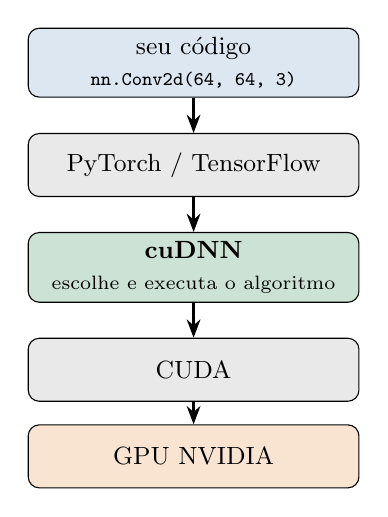
\begin{tikzpicture}[font=\small,>={Stealth},
        c/.style={draw,rounded corners,minimum width=4.2cm,minimum height=0.8cm,align=center}]
      \node[c,fill=azul!15] (a) at (0,3.3) {seu código\\{\scriptsize\texttt{nn.Conv2d(64, 64, 3)}}};
      \node[c,fill=cinza!15] (b) at (0,2.0) {PyTorch / TensorFlow};
      \node[c,fill=verde!25] (c) at (0,0.7) {\textbf{cuDNN}\\{\scriptsize escolhe e executa o algoritmo}};
      \node[c,fill=cinza!15] (d) at (0,-0.6) {CUDA};
      \node[c,fill=laranja!20] (e) at (0,-1.7) {GPU NVIDIA};
      \foreach \u/\v in {a/b,b/c,c/d,d/e} \draw[->,thick] (\u) -- (\v);
    \end{tikzpicture}
    \column{0.6\textwidth}
    \footnotesize
    \textbf{O que é.} Biblioteca da NVIDIA (\emph{CUDA Deep Neural Network library}) com rotinas otimizadas para GPU: convolução,
    pooling, normalização, ativações. Em GPUs NVIDIA, os frameworks não fazem a conta; chamam a cuDNN.\\[0.5em]
    \textbf{Por que importa aqui.} A \emph{mesma} convolução tem várias implementações: multiplicação de matrizes
    (\emph{im2col} + GEMM, outra forma de escrever a convolução como produto de matrizes, diferente da do slide B.8), FFT, Winograd. A melhor depende do kernel, dos canais, do lote e da GPU.\\[0.5em]
    Por isso a cuDNN pode \textbf{medir} cada opção na primeira execução e guardar a mais rápida para cada camada:\\[0.3em]
    \centering
\begin{verbatim}
torch.backends.cudnn.benchmark = True
\end{verbatim}
  \end{columns}
  \intuicao{como um GPS que testa as rotas possíveis e usa a mais rápida em cada trecho; o destino (o resultado) é o mesmo.}{Chetlur et al., 2014}
\end{frame}

% =====================================================================
\section[9.\enspace Características aleatórias ou não supervisionadas (cap.~9.9)]{Características (\emph{features}) aleatórias ou não supervisionadas \textcolor{cinza}{(cap.~9.9)}}

\begin{frame}{9.1\enspace Kernels sem treino supervisionado: três estratégias}
  \small
  O mais caro no treino de uma CNN é \textbf{aprender as características} (os kernels); a camada de saída é barata, pois após o pooling recebe
  poucas características. Para reduzir o custo, os kernels podem ser obtidos \emph{sem} treino supervisionado:\\[0.3em]
  \centering
  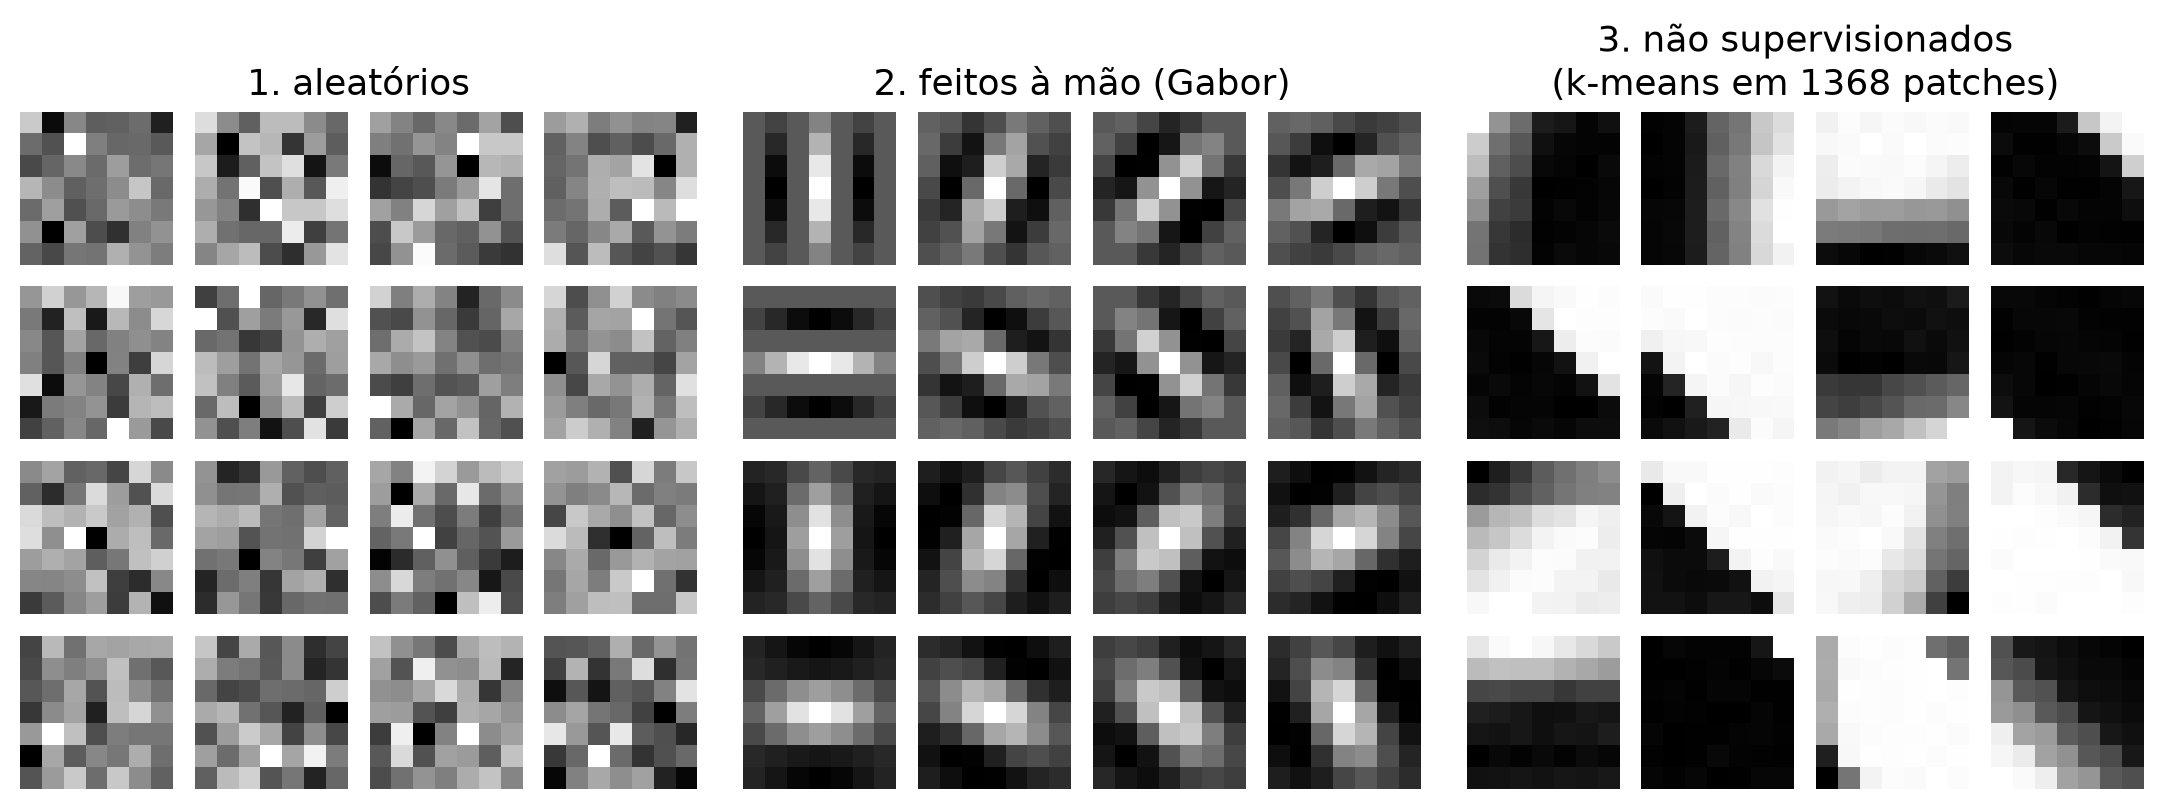
\includegraphics[width=0.76\textwidth]{figuras/bancos_kernels.png}\\[0.2em]
  \raggedright
  \footnotesize
  \textbf{1.} sorteados; \textbf{2.} projetados à mão, como detectores de borda numa orientação e escala (aqui, Gabor);
  \textbf{3.} aprendidos com critério \emph{não supervisionado}: Coates et al.\ (2011) aplicam k-means a pequenos recortes
  (\emph{patches}) e usam cada centroide como kernel (9.2).
  {\scriptsize\textcolor{cinza}{Figura calculada: 16 kernels $7\times7$ por estratégia; k-means sobre as imagens sintéticas dos slides anteriores.}}
\end{frame}

\begin{frame}{9.2\enspace k-means em patches: o que é um centroide}
  \begin{columns}[T]
    \column{0.55\textwidth}
    \centering
    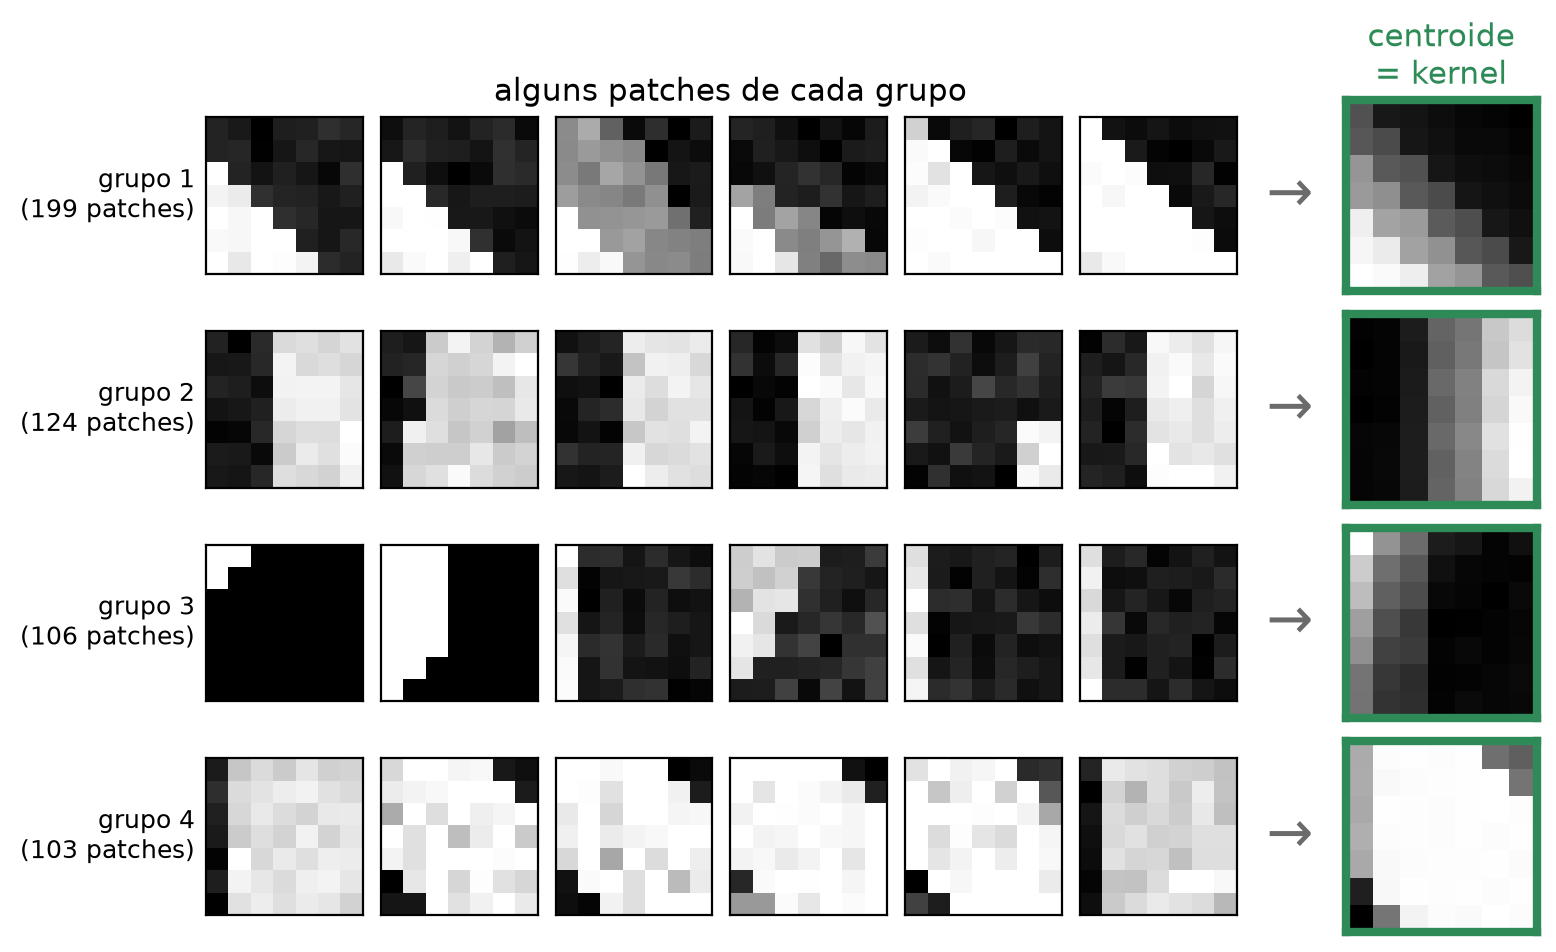
\includegraphics[width=\linewidth]{figuras/kmeans_grupos.png}\\[0.2em]
    {\scriptsize\textcolor{cinza}{Calculado: 1368 patches, $k=16$; 4 grupos mostrados.}}
    \column{0.43\textwidth}
    \footnotesize
    Cada \emph{patch} $7\times7$ vira um vetor de 49 números. O k-means divide os patches em $k$ grupos, repetindo até estabilizar:
    \begin{enumerate}
      \item cada patch vai para o grupo do centroide mais próximo;
      \item cada centroide vira a \textbf{média} do seu grupo: $\mu_j = \frac{1}{|G_j|}\sum_{p\in G_j} p$.
    \end{enumerate}
    O \textbf{centroide} é o patch médio do grupo, a sua forma típica (uma borda vertical, uma diagonal\ldots).\\[0.3em]
    Como também é $7\times7$, serve \textbf{diretamente como kernel}: responde forte onde a imagem se parece com o grupo.
    Nenhum rótulo é usado.
  \end{columns}
  \intuicao{juntando centenas de fotos de rostos e calculando o ``rosto médio'', esse rosto médio é o centroide do grupo.}{Coates et al., 2011; Bishop, 2006, seç.~9.1}
\end{frame}

\begin{frame}{9.3\enspace Características fixas: extrair uma vez, treinar só a última camada}
  \centering
  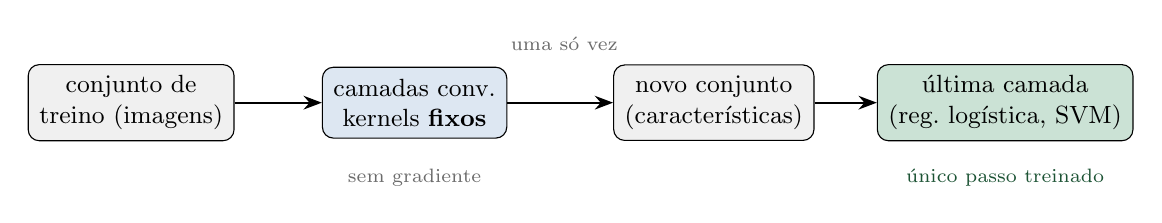
\begin{tikzpicture}[font=\small,>={Stealth},
      b/.style={draw,rounded corners,minimum height=0.9cm,inner sep=4pt,align=center}]
    \node[b,fill=cinza!10] (x) at (0,0) {conjunto de\\treino (imagens)};
    \node[b,fill=azul!15] (f) at (3.6,0) {camadas conv.\\kernels \textbf{fixos}};
    \node[b,fill=cinza!10] (z) at (7.4,0) {novo conjunto\\(características)};
    \node[b,fill=verde!25] (c) at (11.1,0) {última camada\\(reg.\ logística, SVM)};
    \draw[->,thick] (x) -- (f); \draw[->,thick] (f) -- (z); \draw[->,thick] (z) -- (c);
    \node[font=\scriptsize,text=cinza] at (3.6,-0.95) {sem gradiente};
    \node[font=\scriptsize,text=cinza] at (5.5,0.75) {uma só vez};
    \node[font=\scriptsize,text=verde!60!black] at (11.1,-0.95) {único passo treinado};
  \end{tikzpicture}\\[0.8em]
  \raggedright
  \begin{columns}[T]
    \column{0.48\textwidth}
    \footnotesize
    \textbf{Por que é barato.} Se as características não dependem do classificador, elas são determinadas \emph{separadamente}. Basta
    passar o conjunto de treino pelas camadas convolucionais uma única vez e guardar as saídas.
    \column{0.48\textwidth}
    \footnotesize
    \textbf{Por que é mais fácil.} Com as características fixas, treinar a última camada costuma ser um problema de otimização
    \textbf{convexo}, quando ela é uma regressão logística ou uma SVM: qualquer mínimo local é global, sem as dificuldades do treino de
    uma rede profunda.
  \end{columns}
  \intuicao{congela-se o ``olho'' da rede e treina-se só quem decide a partir do que ele vê.}{Goodfellow et al., 2016, seç.~9.9}
\end{frame}

\begin{frame}{9.4\enspace Por que pesos aleatórios funcionam surpreendentemente bem}
  \small
  Filtros aleatórios muitas vezes funcionam surpreendentemente bem em CNNs (Jarrett et al., 2009; Pinto et al., 2011). Saxe et al.\ (2011) mostraram por quê: com
  pesos aleatórios, \textbf{convolução seguida de pooling} já é \textbf{seletiva em frequência} e \textbf{invariante à translação}.\\[0.2em]
  \centering
  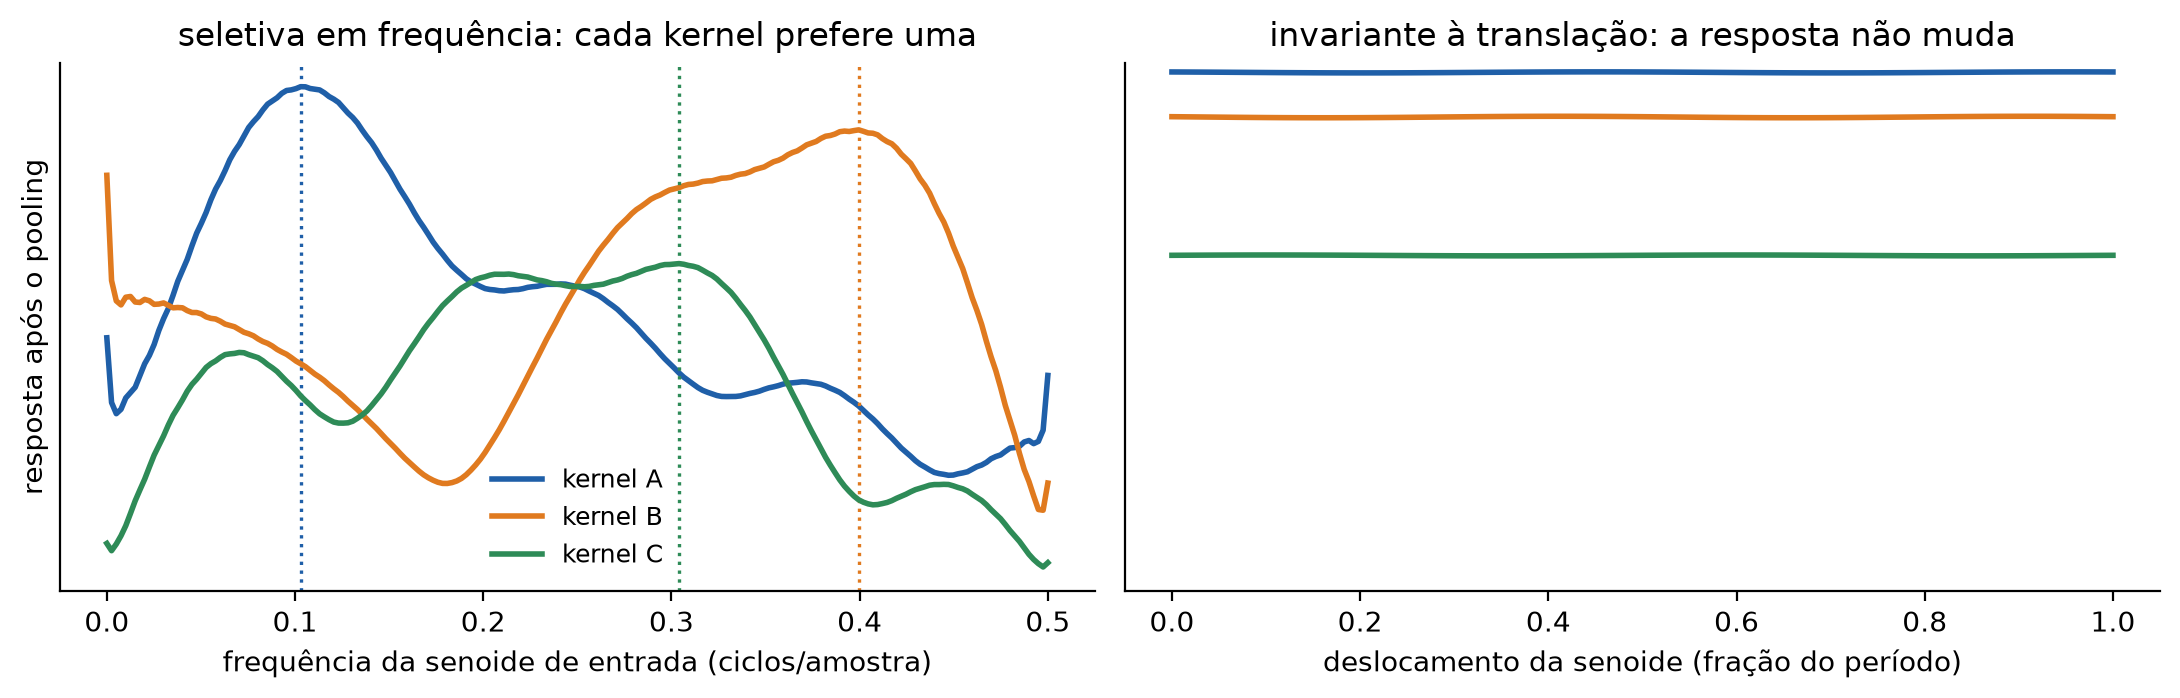
\includegraphics[width=0.74\textwidth]{figuras/pesos_aleatorios.png}\\[0.1em]
  \raggedright
  \footnotesize
  Calculado: 3 kernels 1D aleatórios (9 pesos), entrada senoidal, pooling quadrático sobre toda a saída.
  \textbf{Uso prático:} comparar \emph{arquiteturas} treinando só a última camada de cada uma; treinar por completo só a melhor.
  \intuicao{boa parte do desempenho vem da arquitetura (convolução + pooling), não só dos valores dos pesos.}{Saxe et al., 2011}
\end{frame}

\begin{frame}{9.5\enspace Pré-treinamento camada a camada e o que se faz hoje}
  \begin{columns}[T]
    \column{0.5\textwidth}
    \footnotesize
    \textbf{Pré-treinamento guloso.} Aprender as características sem propagar pela rede inteira a cada passo:
    \begin{enumerate}
      \item treinar a 1.\textsuperscript{a} camada isoladamente;
      \item extrair suas features uma só vez;
      \item treinar a 2.\textsuperscript{a} sobre elas, e assim por diante.
    \end{enumerate}
    Exemplo canônico: a \emph{convolutional deep belief network} (Lee et al., 2009).\\[0.3em]
    \textbf{Um passo além.} Treina-se um modelo de um \emph{patch} pequeno (como o k-means) e usam-se seus parâmetros como kernels:
    a rede é treinada \alert{sem usar convolução}, e o custo alto fica só na inferência.
    \column{0.46\textwidth}
    \footnotesize
    \begin{block}{Popular de 2007 a 2013 (aprox.)}
      Conjuntos rotulados pequenos e poder computacional limitado.
    \end{block}
    \begin{block}{Hoje}
      A maioria das CNNs é treinada de forma \textbf{puramente supervisionada}, com retropropagação pela rede inteira a cada iteração.
    \end{block}
    \begin{block}{Questão em aberto}
      O ganho vem de \emph{regularização}, ou só de permitir arquiteturas \emph{maiores}, por ser mais barato? Ainda é difícil separar.
    \end{block}
  \end{columns}
  {\scriptsize\textcolor{cinza}{Goodfellow et al.\ (2016), seç.~9.9 e cap.~15; Coates et al.\ (2011); Lee et al.\ (2009).}}
\end{frame}

% =====================================================================
\section[10.\enspace A base neurocientífica das redes convolucionais (cap.~9.10)]{A base neurocientífica das redes convolucionais \textcolor{cinza}{(cap.~9.10)}}

\begin{frame}{10.1\enspace Hubel e Wiesel: o ponto de partida}
  \small
  As redes convolucionais talvez sejam o maior caso de sucesso da IA inspirada na biologia. Parte central dessa inspiração vem de
  \textbf{Hubel e Wiesel} (1959, 1962, 1968; Nobel de 1981): registrando neurônios individuais do córtex visual de gatos, viram que
  muitos respondiam fortemente a padrões de luz muito específicos, como \textbf{barras com uma orientação precisa}, e quase nada a
  outros padrões.\\[0.6em]
  \centering
  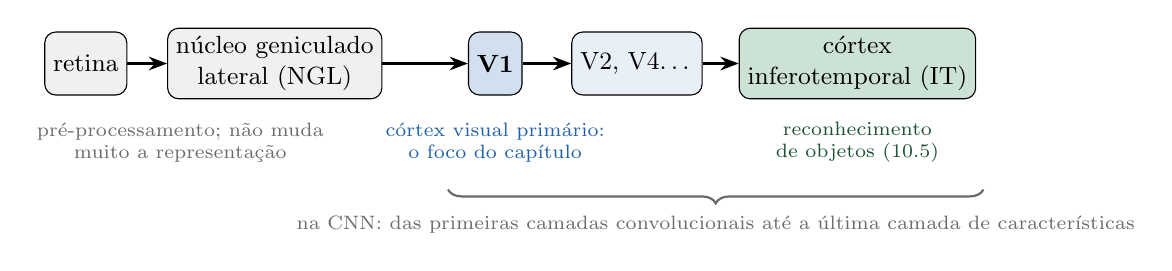
\begin{tikzpicture}[font=\small,>={Stealth},
      b/.style={draw,rounded corners,minimum height=0.8cm,inner sep=3pt,align=center}]
    \node[b,fill=cinza!10] (r) at (0,0) {retina};
    \node[b,fill=cinza!10] (n) at (2.4,0) {núcleo geniculado\\lateral (NGL)};
    \node[b,fill=azul!20] (v1) at (5.2,0) {\textbf{V1}};
    \node[b,fill=azul!10] (v2) at (7.0,0) {V2, V4\ldots};
    \node[b,fill=verde!25] (it) at (9.8,0) {córtex\\inferotemporal (IT)};
    \foreach \u/\v in {r/n,n/v1,v1/v2,v2/it} \draw[->,thick] (\u) -- (\v);
    \node[font=\scriptsize,text=cinza,align=center] at (1.2,-1.0) {pré-processamento; não muda\\muito a representação};
    \node[font=\scriptsize,text=azul,align=center] at (5.2,-1.0) {córtex visual primário:\\o foco do capítulo};
    \node[font=\scriptsize,text=verde!60!black,align=center] at (9.8,-1.0) {reconhecimento\\de objetos (10.5)};
    \draw[decorate,decoration={brace,amplitude=5pt,mirror},thick,cinza] (4.6,-1.6) -- (11.4,-1.6)
      node[midway,below=6pt,font=\scriptsize,text=cinza] {na CNN: das primeiras camadas convolucionais até a última camada de características};
  \end{tikzpicture}
  \intuicao{a CNN não copia o cérebro; copia alguns princípios de organização da V1, medidos em laboratório.}{Goodfellow et al., 2016, seç.~9.10}
\end{frame}

\begin{frame}{10.2\enspace Três propriedades da V1 que a camada convolucional imita}
  \footnotesize
  \renewcommand{\arraystretch}{1.3}
  \begin{tabular}{@{}p{3.0cm}p{6.6cm}p{4.2cm}@{}}
    \toprule
    \textbf{propriedade da V1} & \textbf{o que significa} & \textbf{na CNN} \\ \midrule
    \textbf{1.\ mapa espacial} & A V1 tem estrutura 2D que espelha a imagem na retina: luz na metade inferior da retina afeta só a
      metade correspondente da V1. & características organizadas em \textbf{mapas 2D} \\
    \textbf{2.\ células simples} & A atividade é aproximadamente uma \textbf{função linear} da imagem num campo receptivo pequeno e
      localizado. & \textbf{unidades detectoras}: convolução (e não linearidade) \\
    \textbf{3.\ células complexas} & Respondem a características parecidas com as das simples, mas são \textbf{invariantes a pequenos
      deslocamentos} dela (e a certas mudanças de iluminação). & \textbf{pooling}; e pooling entre canais (maxout, slide 3.4) \\ \bottomrule
  \end{tabular}\\[0.4em]
  \small
  Os mesmos princípios parecem se repetir nas áreas seguintes: detecção e pooling, várias vezes.
  \intuicao{simples $\approx$ ``há uma borda vertical \emph{exatamente aqui}''; complexa $\approx$ ``há uma borda vertical \emph{por perto}''.}{Goodfellow et al., 2016, seç.~9.10; Hubel e Wiesel, 1962}
\end{frame}

\begin{frame}{10.3\enspace Células simples: funções de Gabor}
  \begin{columns}[T]
    \column{0.5\textwidth}
    \footnotesize
    \textbf{Como se mede.} \emph{Correlação reversa}: mostra-se ruído branco, registra-se a resposta do neurônio e ajusta-se um
    modelo linear; os pesos obtidos são o ``kernel'' do neurônio. Na maioria das células simples da V1, eles são bem descritos por
    uma \textbf{função de Gabor}:
    \[ w(x,y) = \alpha\, e^{-\beta_x x'^2 - \beta_y y'^2} \cos\!\left(f x' + \phi\right) \]
    em que $x'$, $y'$ são as coordenadas giradas pelo ângulo $\tau$ em torno do centro $(x_0,y_0)$.
    \column{0.47\textwidth}
    \centering
    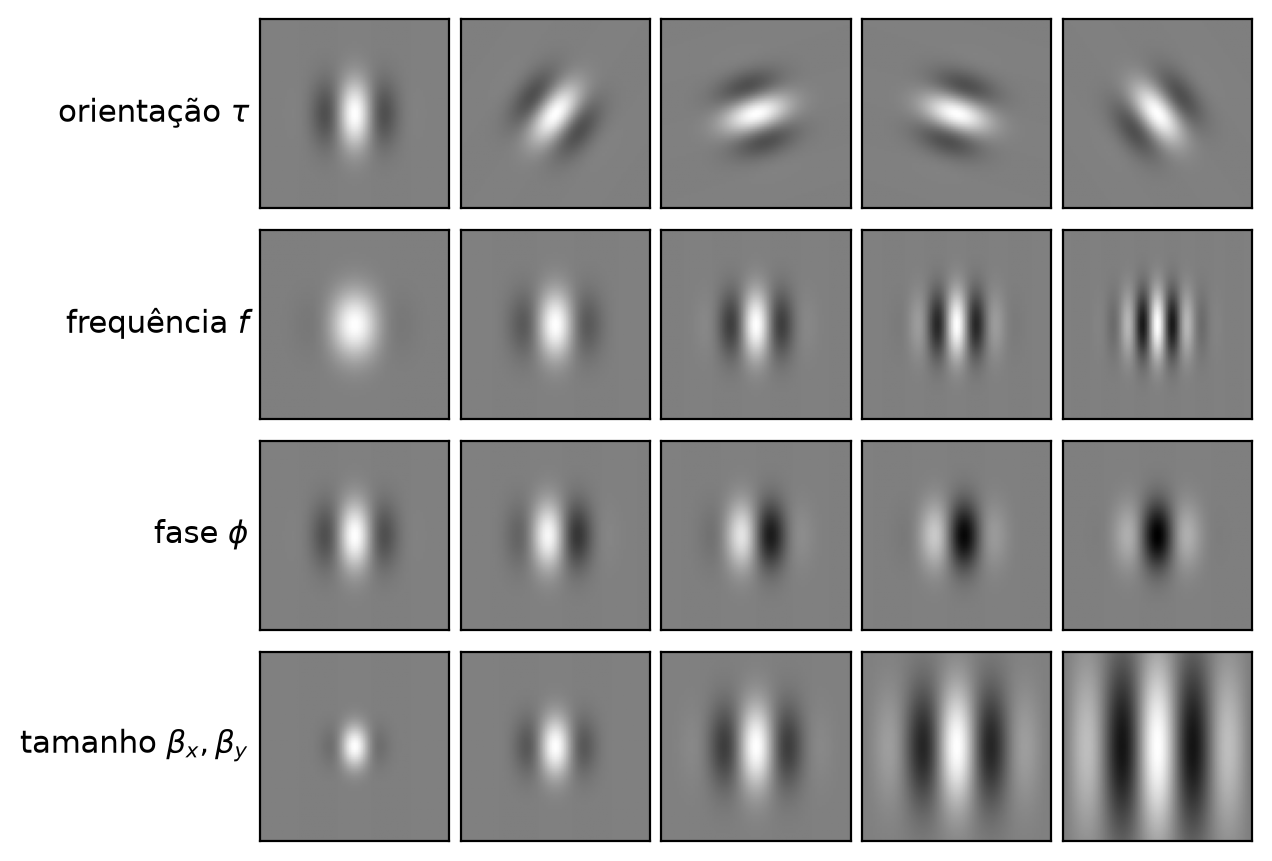
\includegraphics[width=0.82\linewidth]{figuras/gabor_param.png}\\[0.2em]
    \scriptsize
    \begin{tabular}{@{}ll@{}}
      $\alpha$: intensidade & $\beta_x,\beta_y$: tamanho (inverso) \\
      $f$: frequência das listras & $\phi$: fase (onde caem as listras) \\
      $\tau$: orientação & $x_0,y_0$: posição do campo \\
    \end{tabular}
  \end{columns}
  \intuicao{gaussiana $\times$ cosseno: uma ``janela'' que limita \emph{onde} a célula olha, e listras que dizem \emph{o quê} ela procura.}{Goodfellow et al., 2016, seç.~9.10, eq.~9.15--9.17}
\end{frame}

\begin{frame}{10.4\enspace Células complexas: o modelo de energia}
  \small
  Uma célula complexa pode ser modelada combinando duas células simples $s_0$ e $s_1$ com os mesmos parâmetros, exceto a fase,
  deslocada de $1/4$ de ciclo (um \emph{par em quadratura}):
  \[ c(I) = \sqrt{s_0(I)^2 + s_1(I)^2} \]
  \centering
  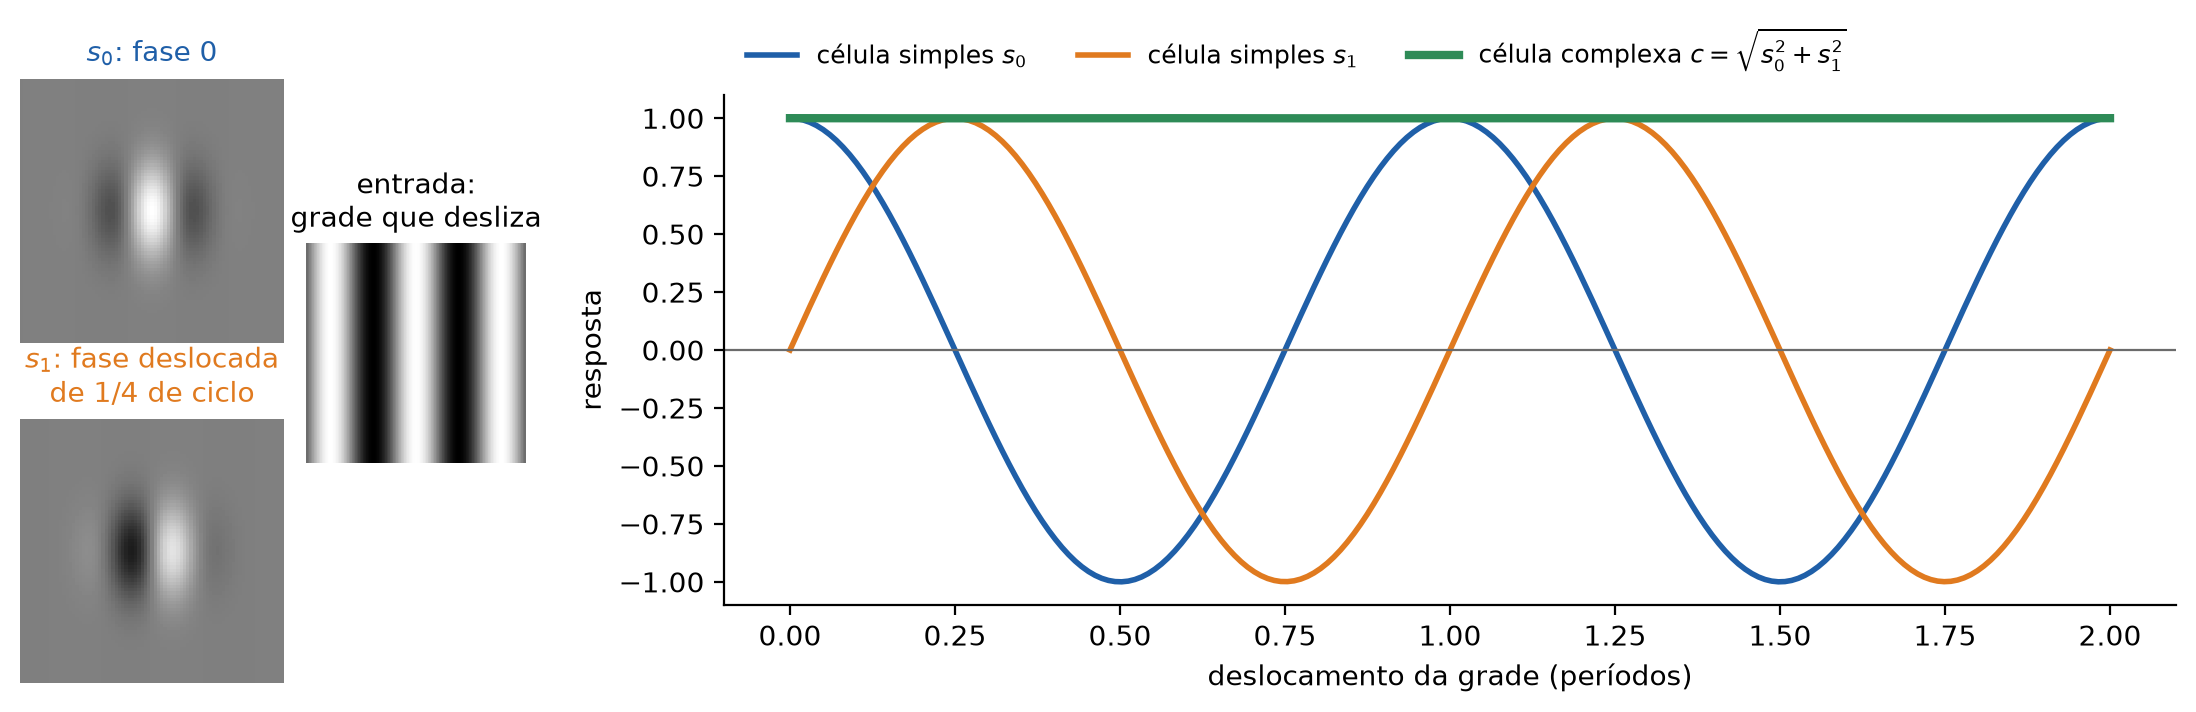
\includegraphics[width=0.58\textwidth]{figuras/celula_complexa.png}\\[0.1em]
  \raggedright
  \footnotesize
  Calculado: com a grade, $c$ fica constante (0,07\%) e não muda com a imagem \textbf{negada} (só entram quadrados);
  em imagens quaisquer, ela é aproximada (pequenos deslocamentos na direção $\tau$).
  \intuicao{é uma forma de pooling quadrático, parente da do slide 9.4, mas sobre dois filtros na mesma posição; na grade, $s_0^2+s_1^2=\cos^2+\sin^2$ não depende do deslocamento.}{Adelson e Bergen, 1985; Goodfellow et al., 2016, seç.~9.10}
\end{frame}

\begin{frame}{10.5\enspace Além da V1: ``células avó'' e o córtex inferotemporal}
  \begin{columns}[T]
    \column{0.5\textwidth}
    \footnotesize
    \textbf{Células avó.} Indo mais fundo no cérebro, encontram-se neurônios que respondem a um conceito específico e são invariantes a
    muitas transformações da entrada. O exemplo famoso é o \textbf{``neurônio Halle Berry''}, no lobo temporal medial de humanos:
    disparava para fotos da atriz, desenhos dela e até o nome escrito, e não para outras pessoas (Quiroga et al., 2005).\\[0.5em]
    Eles são mais gerais que as CNNs do livro, que não generalizariam automaticamente para o nome escrito. Trabalhos posteriores acharam unidades parecidas em modelos multimodais, como o CLIP (Goh et al., 2021).
    \column{0.46\textwidth}
    \footnotesize
    \textbf{Córtex inferotemporal (IT).} É o análogo mais próximo da \emph{última camada de características} de uma CNN.\\[0.5em]
    Para uma visão rápida do objeto, nos \textbf{primeiros $\sim$100\,ms}, antes que o \emph{feedback} de outras áreas pese:
    \begin{itemize}
      \item as CNNs \textbf{predizem as taxas de disparo} de neurônios do IT;
      \item e reconhecem objetos com desempenho semelhante ao de humanos com tempo limitado.
    \end{itemize}
  \end{columns}
  \intuicao{a semelhança é maior na primeira olhada; depois, o cérebro faz muito mais do que uma passagem para a frente.}{DiCarlo, 2013; Yamins et al., 2014}
\end{frame}

\begin{frame}{10.6\enspace Onde a analogia falha}
  \small
  \begin{itemize}
    \item \textbf{Resolução.} O olho tem alta resolução só na \textbf{fóvea} (um polegar a um braço de distância) e compõe a cena com
      \textbf{movimentos sacádicos} e atenção. A CNN recebe a imagem inteira em alta resolução.
    \item \textbf{Integração.} A visão é integrada a outros sentidos, como a audição, e a fatores como humor e pensamento.
    \item \textbf{Tarefa.} O cérebro entende \textbf{cenas inteiras}: relações entre objetos e geometria 3D, não só rótulos.
    \item \textbf{Feedback.} Até a V1 é fortemente influenciada por áreas superiores; em redes, o feedback ainda não trouxe ganho convincente (até 2016, segundo o livro).
    \item \textbf{Neurônios.} Provavelmente usam outras ativações e outros poolings; um neurônio da V1 pode exigir \textbf{vários filtros
      quadráticos} (Rust et al., 2005), e não um só filtro linear.
  \end{itemize}
  \intuicao{o córtex inferotemporal (IT, slide 10.5) e a CNN carregam informação parecida, mas os cálculos intermediários podem ser bem diferentes.}{Goodfellow et al., 2016, seç.~9.10}
\end{frame}

\begin{frame}{10.7\enspace O que a neurociência não disse: como treinar}
  \centering
  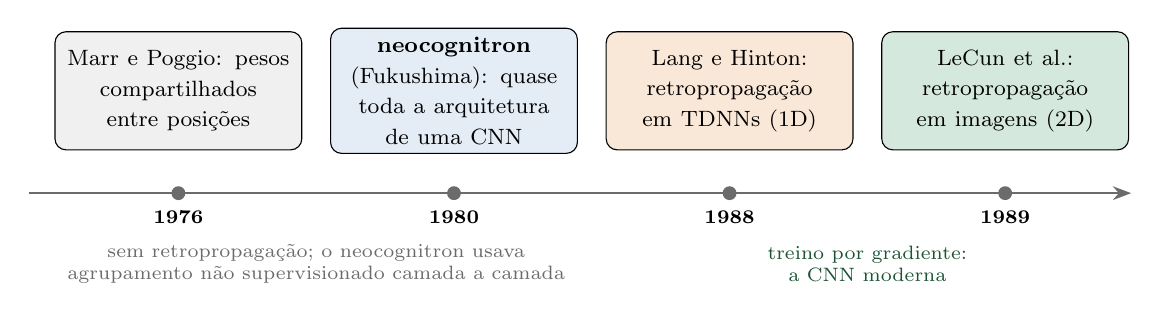
\begin{tikzpicture}[font=\small,>={Stealth},
      e/.style={draw,rounded corners,minimum width=3.1cm,minimum height=1.5cm,align=center,text width=2.9cm}]
    \draw[->,thick,cinza] (-0.4,0) -- (13.6,0);
    \foreach \x/\a in {1.5/1976,5.0/1980,8.5/1988,12.0/1989} { \fill[cinza] (\x,0) circle (2.5pt); \node[below,font=\scriptsize\bfseries] at (\x,-0.1) {\a}; }
    \node[e,fill=cinza!10] at (1.5,1.3) {\footnotesize Marr e Poggio: pesos compartilhados entre posições};
    \node[e,fill=azul!12] at (5.0,1.3) {\footnotesize \textbf{neocognitron} (Fukushima): quase toda a arquitetura de uma CNN};
    \node[e,fill=laranja!18] at (8.5,1.3) {\footnotesize Lang e Hinton: retropropagação em TDNNs (1D)};
    \node[e,fill=verde!20] at (12.0,1.3) {\footnotesize LeCun et al.: retropropagação em imagens (2D)};
    \node[font=\scriptsize,text=cinza,align=center] at (3.25,-0.9) {sem retropropagação; o neocognitron usava\\agrupamento não supervisionado camada a camada};
    \node[font=\scriptsize,text=verde!60!black,align=center] at (10.25,-0.9) {treino por gradiente:\\a CNN moderna};
  \end{tikzpicture}\\[0.8em]
  \raggedright
  \small
  A neurociência forneceu a \textbf{arquitetura} (mapas, detecção local, pooling), mas pouco disse sobre \textbf{como treinar}.
  O ingrediente que faltava, o aprendizado por gradiente com retropropagação, veio de outra linha de pesquisa.
  \intuicao{a biologia deu a planta da casa; o método para construí-la veio da matemática.}{Goodfellow et al., 2016, seç.~9.10}
\end{frame}

\begin{frame}{10.8\enspace Por que tantos algoritmos aprendem ``Gabor''}
  \small
  Em \textbf{imagens naturais}, muitos algoritmos aprendem sozinhos características parecidas com Gabor, como as da V1: codificação esparsa
  (Olshausen e Field, 1996), a 1.\textsuperscript{a} camada de redes profundas e também o k-means, desde que com branqueamento e em imagens naturais.\\[0.2em]
  \centering
  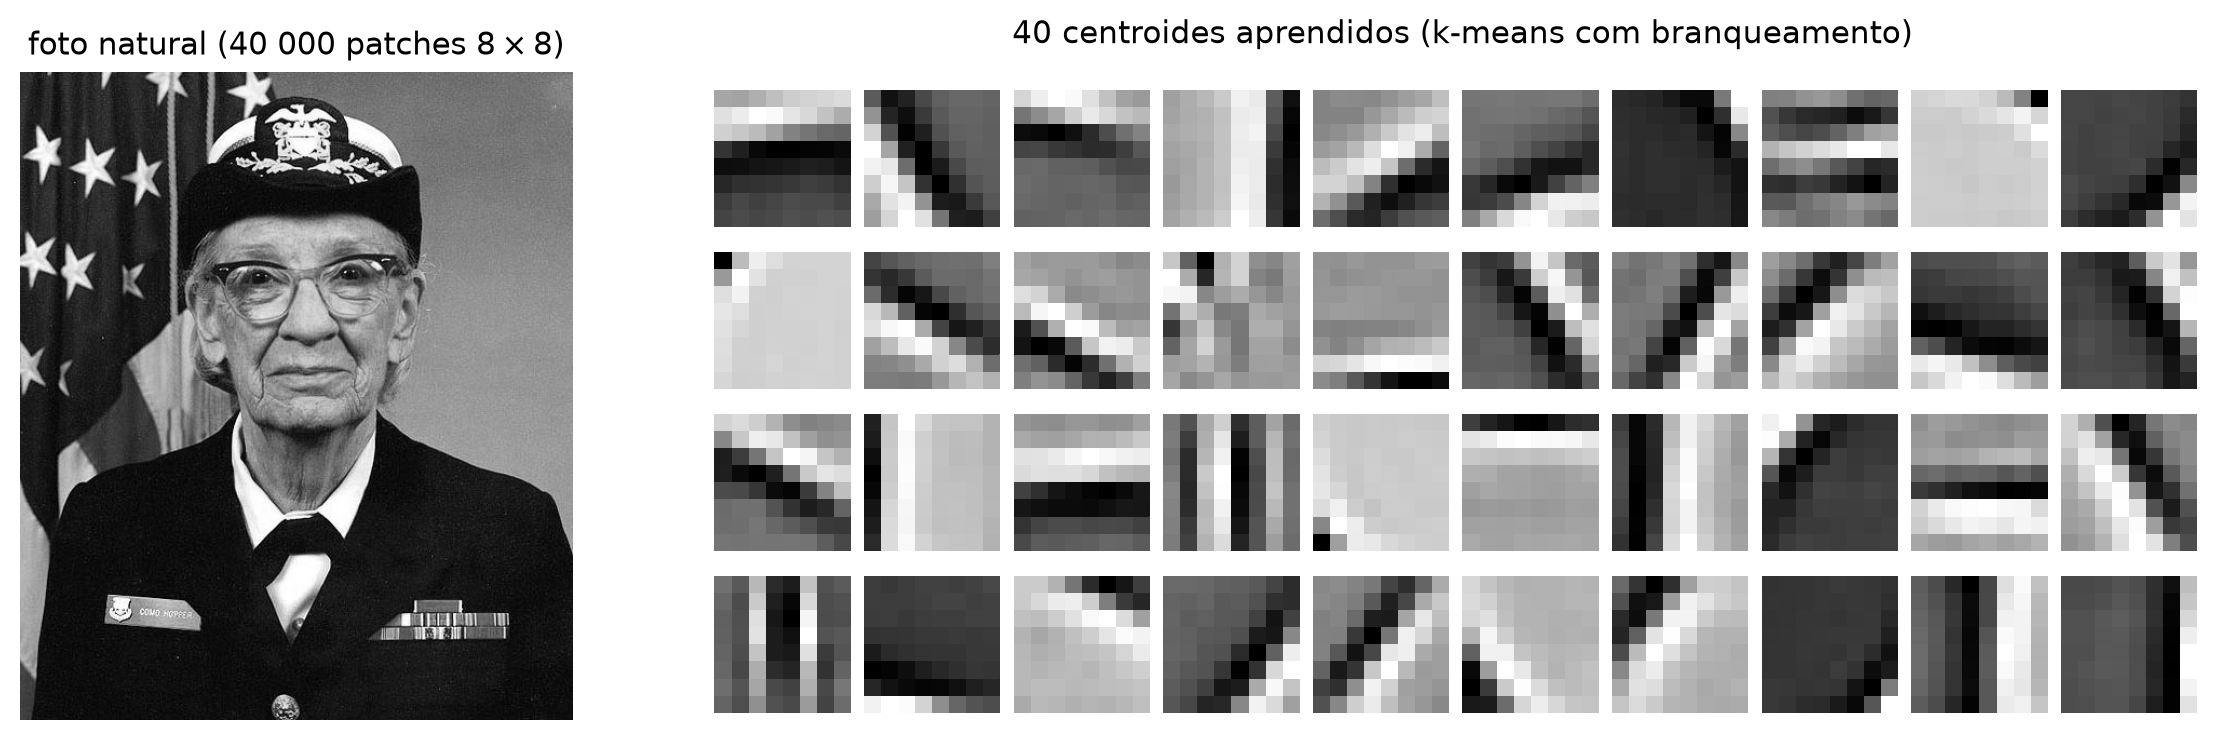
\includegraphics[width=0.74\textwidth]{figuras/gabor_aprendido.png}\\[0.1em]
  \raggedright
  \footnotesize
  Calculado: k-means com branqueamento (Coates e Ng, 2012) numa foto de domínio público (Grace Hopper, Marinha dos EUA): surgem bordas \textbf{localizadas e orientadas}.
  Por isso não dá para dizer qual algoritmo é ``o'' modelo do cérebro; mas um que \emph{não} aprendesse bordas seria mau candidato.
  \intuicao{bordas orientadas fazem parte da estatística das imagens naturais; quem aprende bem com elas as encontra.}{Hyvärinen et al., 2009; Goodfellow et al., 2016, seç.~9.10}
\end{frame}

% =====================================================================
\section[11.\enspace Redes convolucionais e a história do aprendizado profundo (cap.~9.11)]{Redes convolucionais e a história do aprendizado profundo \textcolor{cinza}{(cap.~9.11)}}

\begin{frame}{11.1\enspace As CNNs abriram o caminho}
  \centering
  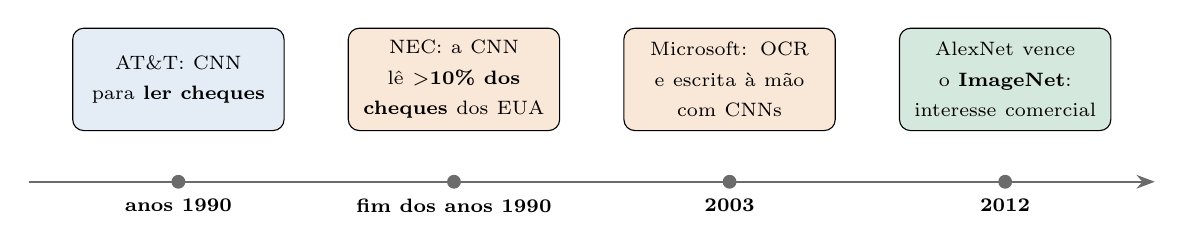
\begin{tikzpicture}[font=\small,>={Stealth},
      e/.style={draw,rounded corners,minimum width=2.6cm,minimum height=1.3cm,align=center,text width=2.45cm}]
    \draw[->,thick,cinza] (-0.3,0) -- (14.0,0);
    \foreach \x/\a in {1.6/anos 1990,5.1/fim dos anos 1990,8.6/2003,12.1/2012} { \fill[cinza] (\x,0) circle (2.5pt); \node[below,font=\scriptsize\bfseries] at (\x,-0.1) {\a}; }
    \node[e,fill=azul!12] at (1.6,1.3) {\scriptsize AT\&T: CNN para \textbf{ler cheques}};
    \node[e,fill=laranja!18] at (5.1,1.3) {\scriptsize NEC: a CNN lê \textbf{$>$10\% dos cheques} dos EUA};
    \node[e,fill=laranja!18] at (8.6,1.3) {\scriptsize Microsoft: OCR e escrita à mão com CNNs};
    \node[e,fill=verde!20] at (12.1,1.3) {\scriptsize AlexNet vence o \textbf{ImageNet}: interesse comercial};
  \end{tikzpicture}\\[0.8em]
  \raggedright
  \small
  \begin{itemize}
    \item As CNNs são um exemplo bem-sucedido de ideias tiradas do estudo do cérebro (seção 10).
    \item Estiveram entre os \textbf{primeiros modelos profundos a funcionar bem}, muito antes de redes profundas arbitrárias serem
      consideradas viáveis, e entre as primeiras treinadas com sucesso por retropropagação.
    \item Também foram das primeiras a resolver \textbf{aplicações comerciais} importantes, e já venciam competições anos antes de 2012.
  \end{itemize}
  {\scriptsize\textcolor{cinza}{Goodfellow et al.\ (2016), seç.~9.11; LeCun et al.\ (1989, 1998); Simard et al.\ (2003); Krizhevsky et al.\ (2012).}}
\end{frame}

\begin{frame}{11.2\enspace Por que funcionaram antes, e o que vem depois}
  \begin{columns}[T]
    \column{0.55\textwidth}
    \footnotesize
    \textbf{Por que as CNNs deram certo quando as redes densas com retropropagação eram tidas como um fracasso?}
    Não está claro. Hipóteses do livro:
    \begin{itemize}
      \footnotesize
      \item \textbf{Eficiência}: com menos operações e parâmetros (seções 2 e 8), dava para rodar mais experimentos e ajustar
        implementação e hiperparâmetros.
      \item \textbf{Tamanho}: redes maiores parecem mais fáceis de treinar. Com hardware moderno, redes densas grandes têm desempenho razoável em muitas tarefas, mesmo com os dados e as ativações da época em que se achava que elas não funcionavam.
      \item \textbf{Barreira psicológica}: talvez os praticantes não esperassem que redes neurais funcionassem e não se esforçassem a sério.
    \end{itemize}
    \column{0.41\textwidth}
    \begin{block}{O papel delas}
      \footnotesize As CNNs ``carregaram a tocha'' do aprendizado profundo e abriram caminho para a aceitação das redes neurais em geral.
    \end{block}
    \begin{block}{O que vem depois}
      \footnotesize Elas especializam as redes para dados com \textbf{topologia de grade} (sobretudo imagens 2D) e permitem escalá-las.
      Para \textbf{sequências 1D}, o livro passa a outra especialização: as \textbf{redes recorrentes} (cap.~10).
    \end{block}
  \end{columns}
  \intuicao{as CNNs estiveram entre as primeiras a provar que uma rede profunda bem estruturada podia funcionar na prática.}{Goodfellow et al., 2016, seç.~9.11}
\end{frame}

\begin{frame}[allowframebreaks]{Referências}
  \footnotesize
  \begin{itemize}
    \item I. Goodfellow, Y. Bengio, A. Courville. \emph{Deep Learning}. MIT Press, 2016. Cap. 9.
    \item C. T. Lewis, C. Short. \emph{A Latin Dictionary}. Oxford: Clarendon Press, 1879.
    \item \emph{Oxford English Dictionary}. Oxford University Press. Verbete ``convolution''.
    \item A. Zhang, Z. C. Lipton, M. Li, A. J. Smola. \emph{Dive into Deep Learning} (D2L). Cambridge University Press, 2023. Caps. 7 e 8. \url{https://d2l.ai}
    \item A. V. Oppenheim, A. S. Willsky, S. H. Nawab. \emph{Signals and Systems}. 2.\textsuperscript{a} ed. Prentice Hall, 1997.
    \item A. V. Oppenheim, R. W. Schafer. \emph{Discrete-Time Signal Processing}. 3.\textsuperscript{a} ed. Pearson, 2010.
    \item R. C. Gonzalez, R. E. Woods. \emph{Digital Image Processing}. 4.\textsuperscript{a} ed. Pearson, 2018.
    \item T. H. Cormen, C. E. Leiserson, R. L. Rivest, C. Stein. \emph{Introduction to Algorithms}. 3.\textsuperscript{a} ed. MIT Press, 2009.
    \item V. Dumoulin, F. Visin. A guide to convolution arithmetic for deep learning. arXiv:1603.07285, 2016.
    \item M. Mathieu, M. Henaff, Y. LeCun. Fast training of convolutional networks through FFTs. ICLR, 2014.
    \item A. Coates, A. Ng, H. Lee. An analysis of single-layer networks in unsupervised feature learning. AISTATS, 2011.
    \item A. Coates, A. Y. Ng. Learning feature representations with k-means. In: \emph{Neural Networks: Tricks of the Trade}, 2.\textsuperscript{a} ed., Springer, 2012.
    \item D. H. Hubel, T. N. Wiesel. Receptive fields of single neurones in the cat's striate cortex. \emph{J. Physiol.}, 148:574--591, 1959.
    \item D. H. Hubel, T. N. Wiesel. Receptive fields, binocular interaction and functional architecture in the cat's visual cortex. \emph{J. Physiol.}, 160:106--154, 1962.
    \item D. H. Hubel, T. N. Wiesel. Receptive fields and functional architecture of monkey striate cortex. \emph{J. Physiol.}, 195:215--243, 1968.
    \item E. H. Adelson, J. R. Bergen. Spatiotemporal energy models for the perception of motion. \emph{JOSA A}, 2(2):284--299, 1985.
    \item G. Goh et al. Multimodal neurons in artificial neural networks. \emph{Distill}, 2021.
    \item R. Q. Quiroga, L. Reddy, G. Kreiman, C. Koch, I. Fried. Invariant visual representation by single neurons in the human brain. \emph{Nature}, 435:1102--1107, 2005.
    \item J. J. DiCarlo. Mechanisms underlying visual object recognition: humans vs.\ neurons vs.\ machines. Tutorial, NIPS, 2013.
    \item D. L. K. Yamins et al. Performance-optimized hierarchical models predict neural responses in higher visual cortex. \emph{PNAS}, 111(23):8619--8624, 2014.
    \item N. C. Rust, O. Schwartz, J. A. Movshon, E. P. Simoncelli. Spatiotemporal elements of macaque V1 receptive fields. \emph{Neuron}, 46:945--956, 2005.
    \item D. Marr, T. Poggio. Cooperative computation of stereo disparity. \emph{Science}, 194:283--287, 1976.
    \item K. J. Lang, G. E. Hinton. The development of the time-delay neural network architecture for speech recognition. Relatório CMU-CS-88-152, 1988.
    \item B. A. Olshausen, D. J. Field. Emergence of simple-cell receptive field properties by learning a sparse code for natural images. \emph{Nature}, 381:607--609, 1996.
    \item A. Hyvärinen, J. Hurri, P. O. Hoyer. \emph{Natural Image Statistics}. Springer, 2009.
    \item P. O. Hoyer, A. Hyvärinen. Independent component analysis applied to feature extraction from colour and stereo images. \emph{Network: Computation in Neural Systems}, 11(3):191--210, 2000.
    \item I. J. Goodfellow, A. Courville, Y. Bengio. Scaling up spike-and-slab models for unsupervised feature learning. \emph{IEEE TPAMI}, 35(8):1902--1914, 2013.
    \item C. M. Bishop. \emph{Pattern Recognition and Machine Learning}. Springer, 2006.
    \item A. M. Saxe, P. W. Koh, Z. Chen, M. Bhand, B. Suresh, A. Y. Ng. On random weights and unsupervised feature learning. ICML, 2011.
    \item K. Jarrett, K. Kavukcuoglu, M. Ranzato, Y. LeCun. What is the best multi-stage architecture for object recognition? ICCV, 2009.
    \item N. Pinto, Y. Barhomi, D. D. Cox, J. J. DiCarlo. Comparing state-of-the-art visual features on invariant object recognition tasks. WACV, 2011.
    \item H. Lee, R. Grosse, R. Ranganath, A. Y. Ng. Convolutional deep belief networks for scalable unsupervised learning of hierarchical representations. ICML, 2009.
    \item S. Winograd. \emph{Arithmetic Complexity of Computations}. SIAM, 1980.
    \item A. Lavin, S. Gray. Fast algorithms for convolutional neural networks. CVPR, 2016.
    \item A. G. Howard et al. MobileNets: efficient convolutional neural networks for mobile vision applications. arXiv:1704.04861, 2017.
    \item F. Chollet. Xception: deep learning with depthwise separable convolutions. CVPR, 2017.
    \item S. Chetlur et al. cuDNN: efficient primitives for deep learning. arXiv:1410.0759, 2014.
    \item A. Azulay, Y. Weiss. Why do deep convolutional networks generalize so poorly to small image transformations? \emph{JMLR}, 20(184), 2019.
    \item M. Lin, Q. Chen, S. Yan. Network in network. ICLR, 2014.
    \item P. H. O. Pinheiro, R. Collobert. Recurrent convolutional neural networks for scene labeling. ICML, 2014.
    \item I. Goodfellow, D. Warde-Farley, M. Mirza, A. Courville, Y. Bengio. Maxout networks. ICML, 2013.
    \item K. Fukushima. Neocognitron: a self-organizing neural network model for a mechanism of pattern recognition unaffected by shift in position. \emph{Biological Cybernetics}, 36(4):193--202, 1980.
    \item Y. LeCun et al. Backpropagation applied to handwritten zip code recognition. \emph{Neural Computation}, 1(4):541--551, 1989.
    \item Y. LeCun, L. Bottou, Y. Bengio, P. Haffner. Gradient-based learning applied to document recognition. \emph{Proc. IEEE}, 86(11):2278--2324, 1998.
    \item P. Y. Simard, D. Steinkraus, J. C. Platt. Best practices for convolutional neural networks applied to visual document analysis. ICDAR, 2003.
    \item A. Krizhevsky, I. Sutskever, G. Hinton. ImageNet classification with deep convolutional neural networks. NIPS, 2012.
    \item K. Simonyan, A. Zisserman. Very deep convolutional networks for large-scale image recognition. ICLR, 2015.
    \item M. D. Zeiler, R. Fergus. Visualizing and understanding convolutional networks. ECCV, 2014.
    \item C. Szegedy et al. Going deeper with convolutions. arXiv:1409.4842, 2014; CVPR, 2015.
    \item K. He, X. Zhang, S. Ren, J. Sun. Deep residual learning for image recognition. CVPR, 2016.
    \item Z. Liu et al. A ConvNet for the 2020s. CVPR, 2022. \url{https://arxiv.org/abs/2201.03545}
    \item \textcolor{cinza}{Material visual de apoio (não acadêmico): Mathspark8. \emph{Convolution Explained Visually --- Finally Understand the Math!} \url{https://www.youtube.com/watch?v=F4Edh2S_I-Q}}
  \end{itemize}
\end{frame}

\begin{frame}[standout]
  Obrigado!\\[0.5em]
  \normalsize Perguntas?
\end{frame}

% =====================================================================
\appendix
\section[Slides de backup]{Slides de backup}

\begin{frame}{B.1\enspace O teorema da convolução}
  \small
  A transformada de Fourier $\mathcal{F}$ escreve um sinal como soma de senoides: $X(f)=\mathcal{F}\{x\}(f)$ dá a amplitude e a fase
  da frequência $f$. \textbf{Teorema da convolução:}
  \[
    \mathcal{F}\{x \conv k\} \;=\; \mathcal{F}\{x\}\cdot\mathcal{F}\{k\}
    \qquad\text{\footnotesize(convoluir no tempo = multiplicar ponto a ponto na frequência)}
  \]
  \vspace{-0.6em}
  \begin{columns}[c]
    \column{0.62\textwidth}
    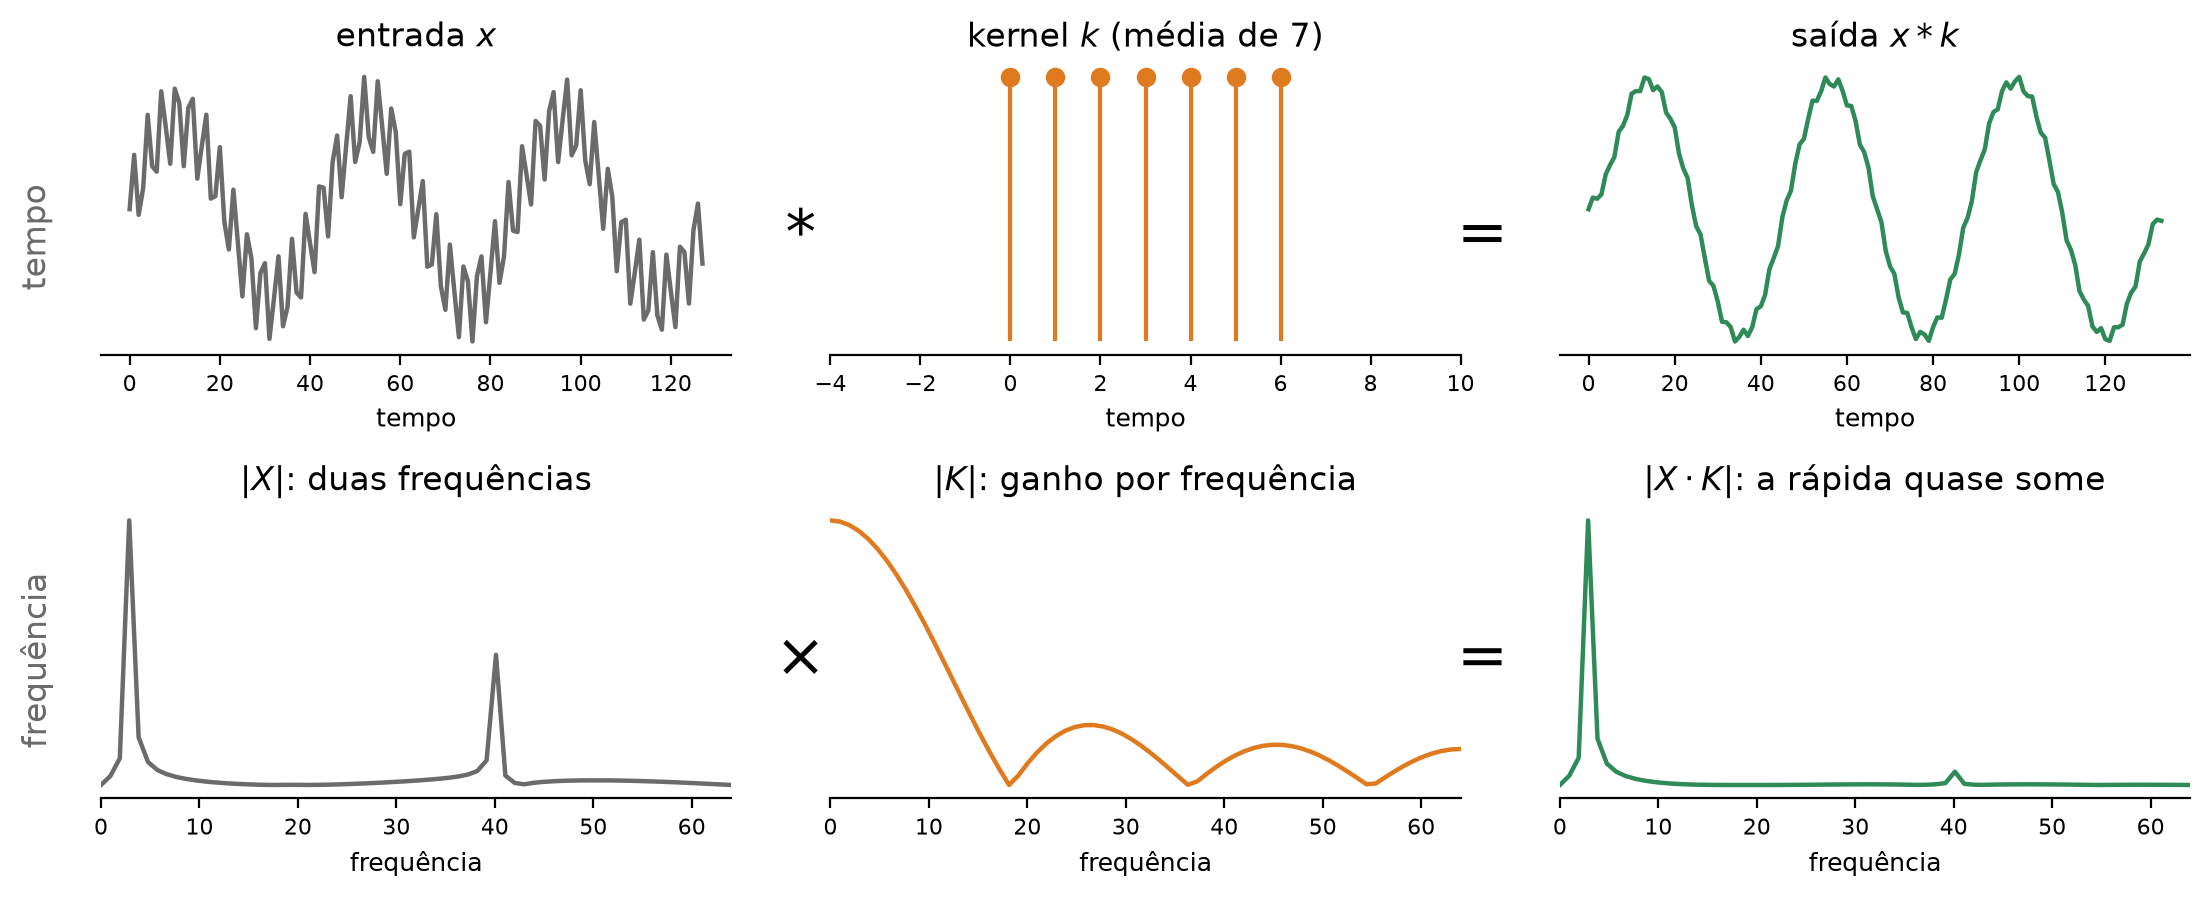
\includegraphics[width=\linewidth]{figuras/fourier.png}
    \column{0.36\textwidth}
    \footnotesize
    \textbf{Exemplo calculado:} $x$ = senoide lenta + rápida; $k$ = média de 7 amostras.\\[0.3em]
    $|K(f)|$ é o \emph{ganho} do kernel em cada frequência: perto de 1 nas baixas, pequeno em $f=40$.\\[0.3em]
    No produto, a componente rápida quase some: a saída fica suave.
  \end{columns}
  \intuicao{como um equalizador: em vez de filtrar amostra a amostra, ajusta-se o ganho de cada frequência.}{Oppenheim e Schafer, 2010, seç.~8.6}
\end{frame}

\begin{frame}{B.2\enspace Convolução via FFT: o algoritmo e o custo}
  \centering
  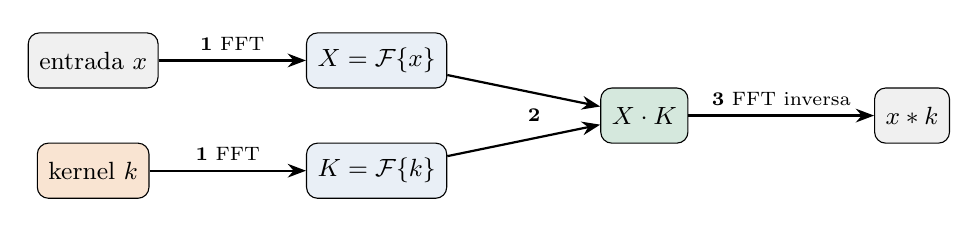
\begin{tikzpicture}[>={Stealth},font=\small,
      b/.style={draw,rounded corners,minimum height=0.7cm,inner sep=4pt,align=center}]
    \node[b,fill=cinza!10] (x) at (0,0.7) {entrada $x$};
    \node[b,fill=laranja!20] (k) at (0,-0.7) {kernel $k$};
    \node[b,fill=azul!10] (fx) at (3.6,0.7) {$X=\mathcal{F}\{x\}$};
    \node[b,fill=azul!10] (fk) at (3.6,-0.7) {$K=\mathcal{F}\{k\}$};
    \node[b,fill=verde!20] (m) at (7.0,0) {$X\cdot K$};
    \node[b,fill=cinza!10] (y) at (10.4,0) {$x \conv k$};
    \draw[->,thick] (x) -- node[above,font=\scriptsize] {\textbf{1} FFT} (fx);
    \draw[->,thick] (k) -- node[above,font=\scriptsize] {\textbf{1} FFT} (fk);
    \draw[->,thick] (fx) -- (m); \draw[->,thick] (fk) -- (m);
    \node[font=\scriptsize] at (5.6,0) {\textbf{2}};
    \draw[->,thick] (m) -- node[above,font=\scriptsize] {\textbf{3} FFT inversa} (y);
  \end{tikzpicture}\\[0.1em]
  \raggedright
  \begin{columns}[T]
    \column{0.5\textwidth}
    \footnotesize
    \textbf{Preenchimento com zeros.} A transformada discreta trata o sinal como periódico; sem cuidado, dá a convolução
    \emph{circular}. Completando $x$ e $k$ com zeros até $L\ge N+M-1$, obtém-se a convolução linear.\\[0.4em]
    \textbf{Correlação cruzada} (slide 1.10): basta espelhar o kernel antes da FFT.\\[0.4em]
    \textbf{Custo.} Direto: $N\cdot M$. Via FFT: três transformadas de $O(L\log L)$ e $L$ produtos.
    \column{0.46\textwidth}
    \footnotesize
    \centering
    Operações, 1D, $N=1024$, $L=2048$\\ {\scriptsize(ordem de grandeza; 1 operação complexa $=$ 1)}\\[0.3em]
    \begin{tabular}{lrr}
      \toprule
      kernel & direto & via FFT \\ \midrule
      $M=3$   & $3\times10^{3}$ & $7\times10^{4}$ \\
      $M=511$ & $5\times10^{5}$ & $7\times10^{4}$ \\ \bottomrule
    \end{tabular}\\[0.4em]
    \raggedright
    O custo da FFT quase não depende de $M$: num só sinal, compensa para \textbf{kernels grandes}. Com muitos canais (8.2), as transformadas
    se diluem, mas a memória a torna rara com $3\times3$ (8.3).
  \end{columns}
  {\scriptsize\textcolor{cinza}{Goodfellow et al.\ (2016), seç.~9.8; Oppenheim e Schafer (2010), seç.~8.7; Cormen et al.\ (2009), cap.~30.}}
\end{frame}

\begin{frame}{B.3\enspace Kernels separáveis}
  \begin{columns}[c]
    \column{0.5\textwidth}
    \centering
    \small
    O Sobel $G_x$ é um \alert{produto externo} de dois vetores:
    \[
      \underbrace{\begin{bmatrix}-1&0&1\\-2&0&2\\-1&0&1\end{bmatrix}}_{3\times3:\ 9\ \text{pesos}}
      =
      \underbrace{\begin{bmatrix}1\\2\\1\end{bmatrix}}_{\text{vertical}}
      \underbrace{\begin{bmatrix}-1&0&1\end{bmatrix}}_{\text{horizontal}}
    \]
    Convoluir com ele $=$ convoluir com $[1,2,1]^{\top}$ nas colunas e depois com $[-1,0,1]$ nas linhas.\\[0.4em]
    \footnotesize por pixel: \textbf{9} multiplicações contra \textbf{3 + 3 = 6}
    \column{0.46\textwidth}
    \footnotesize
    \begin{itemize}
      \item Um kernel de $d$ dimensões é \textbf{separável} quando pode ser escrito como produto externo de $d$ vetores, um por dimensão.
      \item Nesse caso, a convolução em $d$ dimensões vira $d$ convoluções de uma dimensão.
      \item Com largura $w$ em cada dimensão: de $O(w^d)$ para $O(w\cdot d)$, tanto em tempo quanto em parâmetros.
      \item Nem todo kernel é separável. Achar formas mais rápidas, ou aproximadas sem perder acurácia, é pesquisa ativa; até acelerar só a passagem direta já ajuda na implantação.
    \end{itemize}
  \end{columns}
  \intuicao{em vez de pintar um quadrado de uma vez, passa-se o rolo na vertical e depois na horizontal: o resultado é o mesmo, com menos trabalho.}{Goodfellow et al., 2016, seç.~9.8}
\end{frame}

\begin{frame}{B.4\enspace Algoritmo de Winograd \textcolor{cinza}{\normalsize(além do livro)}}
  \begin{columns}[T]
    \column{0.52\textwidth}
    \small
    \textbf{Exemplo 1D:} $F(2,3)$, que calcula 2 saídas com kernel de 3 pesos.\\[0.3em]
    Direto: $y_1 = d_1g_1+d_2g_2+d_3g_3$ e $y_2 = d_2g_1+d_3g_2+d_4g_3$, com \textbf{6} multiplicações.\\[0.3em]
    Winograd: \textbf{4} multiplicações,
    \footnotesize
    \begin{align*}
      m_1 &= (d_1-d_3)\,g_1, & m_2 &= (d_2+d_3)\,\tfrac{g_1+g_2+g_3}{2},\\
      m_3 &= (d_3-d_2)\,\tfrac{g_1-g_2+g_3}{2}, & m_4 &= (d_2-d_4)\,g_3,
    \end{align*}
    \[ y_1 = m_1+m_2+m_3, \qquad y_2 = m_2-m_3-m_4. \]
    \vspace{-1.2em}
    \column{0.44\textwidth}
    \footnotesize
    \textbf{Por que é rápido}
    \begin{itemize}
      \item Troca multiplicações por \emph{somas}, mais baratas.
      \item Termos que só dependem do kernel são calculados \emph{uma vez} e reutilizados em todas as posições.
      \item Resultado \textbf{exato} (a menos de arredondamento).
      \item Em 2D: $F(2{\times}2,3{\times}3)$ usa 16 multiplicações em vez de 36; $F(4{\times}4,3{\times}3)$, 36 em vez de 144.
      \item Blocos maiores economizam mais, mas perdem precisão numérica.
    \end{itemize}
  \end{columns}
  \intuicao{é ideal para os kernels $3\times3$ pequenos, justamente onde a FFT não compensa.}{Lavin e Gray, 2016; Winograd, 1980}
\end{frame}

\begin{frame}{B.5\enspace Convolução separável em profundidade \textcolor{cinza}{\normalsize(além do livro)}}
  \begin{columns}[T]
    \column{0.5\textwidth}
    \centering
    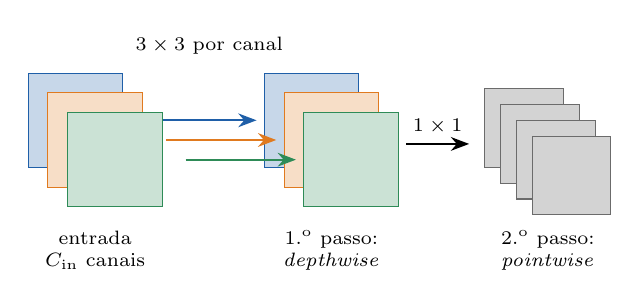
\begin{tikzpicture}[font=\scriptsize,>={Stealth}]
      \foreach \i/\c in {0/azul,1/laranja,2/verde} {
        \fill[\c!25,draw=\c] (0.25*\i,-0.25*\i) rectangle ++(1.2,1.2);
        \fill[\c!25,draw=\c] (3+0.25*\i,-0.25*\i) rectangle ++(1.2,1.2);
        \draw[\c,thick,->] (1.5+0.25*\i,0.6-0.25*\i) -- (2.9+0.25*\i,0.6-0.25*\i);
      }
      \node at (2.3,1.55) {$3\times3$ por canal};
      \node[align=center] at (0.85,-1.05) {entrada\\$C_{\text{in}}$ canais};
      \node[align=center] at (3.85,-1.05) {1.\textsuperscript{o} passo:\\\emph{depthwise}};
      \draw[thick,->] (4.8,0.3) -- node[above] {$1\times1$} (5.6,0.3);
      \foreach \i in {0,1,2,3} \fill[cinza!30,draw=cinza] (5.8+0.2*\i,-0.2*\i) rectangle ++(1.0,1.0);
      \node[align=center] at (6.6,-1.05) {2.\textsuperscript{o} passo:\\\emph{pointwise}};
    \end{tikzpicture}\\[0.6em]
    \footnotesize
    \begin{tabular}{@{}lc@{}}
      \toprule
      & mult. por posição \\ \midrule
      comum & $k^2\,C_{\text{in}}\,C_{\text{out}}$ \\
      em profundidade & $k^2\,C_{\text{in}} + C_{\text{in}}\,C_{\text{out}}$ \\ \bottomrule
    \end{tabular}
    \column{0.46\textwidth}
    \vspace{0.4em}
    \footnotesize
    \textbf{Como funciona}
    \begin{enumerate}
      \item \emph{Depthwise}: um kernel $k\times k$ por canal, sem misturar canais.
      \item \emph{Pointwise}: convolução $1\times1$ (5.2) que mistura os canais.
    \end{enumerate}
    \textbf{Por que é rápido}
    \begin{itemize}
      \item Trata espaço e canais em passos separados.
      \item Razão de custo: $\tfrac{1}{C_{\text{out}}}+\tfrac{1}{k^2}$; com $k=3$, $C_{\text{out}}=64$: cerca de \textbf{8$\times$ menos}.
      \item \alert{Não é exata}: é outra camada, mais restrita, treinada assim desde o início (MobileNet, Xception).
    \end{itemize}
  \end{columns}
  \intuicao{a mesma ideia dos kernels separáveis (B.3), aplicada entre o espaço e os canais.}{Howard et al., 2017; Chollet, 2017}
\end{frame}

\begin{frame}{B.6\enspace Bordas e cores (figura 9.19 do livro)}
  \small
  O livro diz mais: em imagens naturais, muitos algoritmos aprendem características que detectam \textbf{bordas} ou
  \textbf{cores específicas de bordas}. Repetindo o slide 10.8 com patches \emph{coloridos}:\\[0.2em]
  \centering
  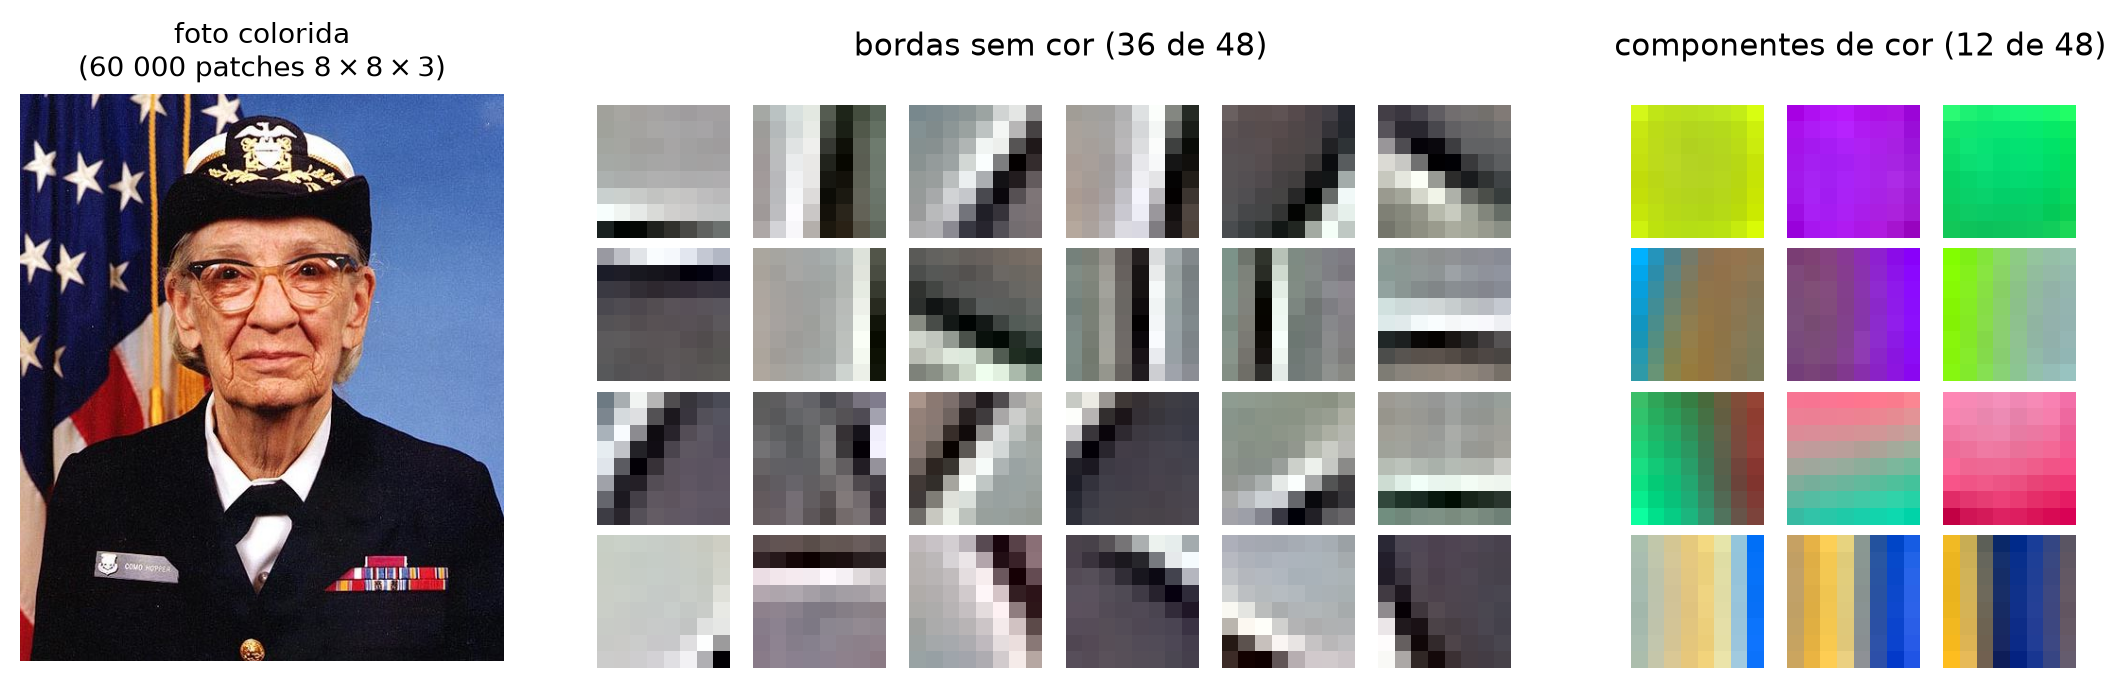
\includegraphics[width=0.64\textwidth]{figuras/gabor_cor.png}\\[0.1em]
  \raggedright
  \begin{columns}[T]
    \column{0.5\textwidth}
    \scriptsize
    \textbf{Duas famílias.} A maioria detecta bordas de \emph{brilho}; uma minoria, \emph{componentes de cor} (manchas e contrastes), mais suaves,
    como em Hoyer e Hyvärinen (2000). ``De cor'': $\ge$30\% da energia cromática.
    \column{0.46\textwidth}
    \scriptsize
    \textbf{Na figura 9.19:} \emph{spike-and-slab sparse coding} (não supervisionado) e a 1.\textsuperscript{a} camada de uma rede
    maxout \emph{supervisionada}. A AlexNet mostra o mesmo (Krizhevsky et al., 2012, fig.~3).
  \end{columns}
  \intuicao{a maioria dos detectores procura ``onde muda o brilho''; alguns procuram ``onde muda a cor''.}{Goodfellow et al., 2016, seç.~9.10, fig.~9.19}
\end{frame}

\begin{frame}{B.7\enspace Desfoque: kernels de média e gaussiano}
  \centering
  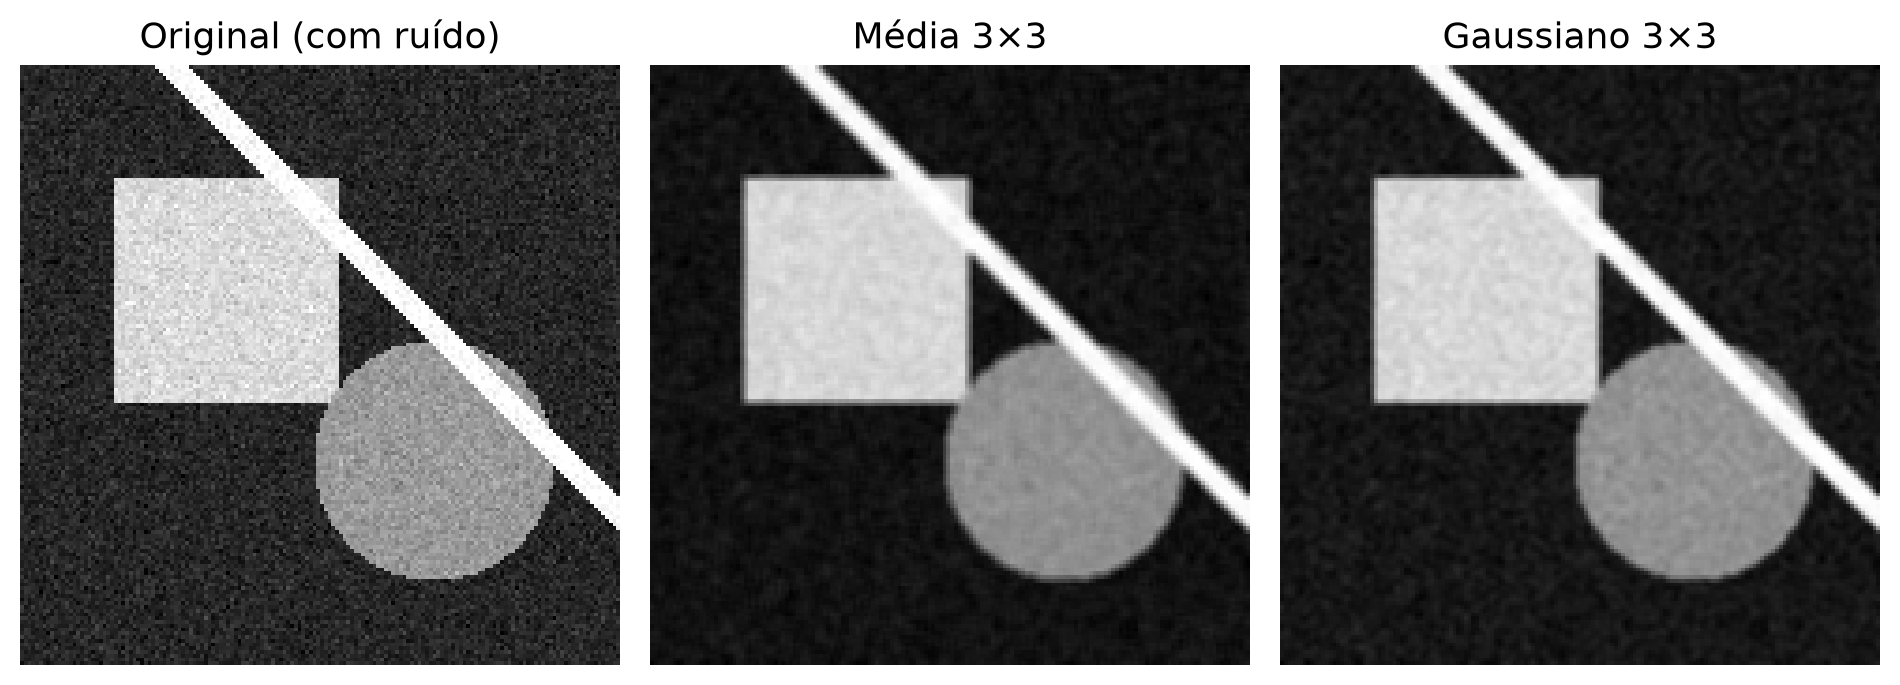
\includegraphics[width=0.46\linewidth]{figuras/desfoque.png}
  \vspace{0.2em}
  \begin{columns}[c]
    \column{0.2\textwidth}
    \centering\footnotesize
    Média (3$\times$3)\\[0.2em]
    $\tfrac{1}{9}\begin{bmatrix}1&1&1\\1&1&1\\1&1&1\end{bmatrix}$
    \column{0.22\textwidth}
    \centering\footnotesize
    Gaussiano (binomial)\\[0.2em]
    $\tfrac{1}{16}\begin{bmatrix}1&2&1\\2&4&2\\1&2&1\end{bmatrix}$
    \column{0.54\textwidth}
    \begin{itemize}\scriptsize
      \item Pesos somam 1: ganho unitário na frequência zero (preserva o brilho médio).
      \item Resposta em frequência da média: aproximadamente um seno cardinal (núcleo de Dirichlet), com lóbulos laterais; a do gaussiano é aproximadamente gaussiana, sem lóbulos (menos artefatos).
      \item \alert{Passa-baixa}: com ruído i.i.d.\ de variância $\sigma^2$, a média $3\times3$ reduz a variância a $\sigma^2/9$, mas também borra as bordas.
      \item[] \textcolor{cinza}{Gonzalez e Woods (2018), seç.~3.5.}
    \end{itemize}
  \end{columns}
  \intuicao{cada pixel vira a média da vizinhança: o ruído, que varia de pixel para pixel, tende a se cancelar; uma borda nítida, também uma variação rápida, é suavizada junto.}{Gonzalez e Woods, 2018, seç.~3.5}
\end{frame}

\begin{frame}{B.8\enspace A convolução como multiplicação por matriz}
  \begin{columns}[c]
    \column{0.5\textwidth}
    \small
    Entrada com 5 valores, kernel $(w_1,w_2,w_3)$, sem padding:
    \[
      \begin{bmatrix} s_1\\ s_2\\ s_3 \end{bmatrix} =
      \begin{bmatrix} w_1&w_2&w_3&0&0\\ 0&w_1&w_2&w_3&0\\ 0&0&w_1&w_2&w_3 \end{bmatrix}
      \begin{bmatrix} x_1\\ x_2\\ x_3\\ x_4\\ x_5 \end{bmatrix}
    \]
    Primeira linha: $s_1 = w_1x_1 + w_2x_2 + w_3x_3$.
    \column{0.46\textwidth}
    \small
    \begin{itemize}
      \item \textbf{Cada linha} é o kernel numa posição.
      \item \textbf{A linha seguinte} é a de cima deslocada uma casa: matriz de \alert{Toeplitz} (pesos repetidos $=$ compartilhados).
      \item \textbf{Os zeros} são as entradas fora da janela: matriz \alert{esparsa}.
    \end{itemize}
  \end{columns}
  \vspace{0.4em}
  \small
  Em 2D, a matriz é duplamente circulante em blocos (Toeplitz em blocos, se a convolução não for circular).
  Consequência: \alert{todo algoritmo de rede neural que funciona com multiplicação por matriz funciona com convolução}, desde que não dependa de propriedades específicas da estrutura da matriz.
  \video{21_convolucao_matriz}
  \intuicao{a convolução é uma camada densa ``amarrada'': a mesma linha de pesos se repete, deslizando, e quase tudo fora dela é zero.}{Goodfellow et al., 2016, seç.~9.1, p.~329}
\end{frame}

\end{document}
